\documentclass[twoside, 12pt, a4paper, english, openany]{book}

\usepackage[utf8]{inputenc}   % Allow UTF-8 input
\usepackage[T1]{fontenc}
\usepackage{lmodern}          % Latin Modern fonts for better output
\usepackage{mathpazo}         % Palatino font for a classic look
\usepackage{mathptmx} % Times-like font
\usepackage{amsmath, amssymb}
\usepackage{graphicx}
\usepackage{enumitem}
\usepackage{float}
\usepackage{soul}
\usepackage{booktabs}
\usepackage[hypcap=false]{caption}
\usepackage{listings}
\lstset{
  language=C++,
  basicstyle=\ttfamily\normalsize, % Bigger font size
  keywordstyle=\color{blue}\bfseries,
  commentstyle=\color{red}\itshape,
  stringstyle=\color{green!60!black},
  numbers=none, % Removed line numbers
  showspaces=false,
  showstringspaces=false,
  showtabs=false,
  frame=single,
  breaklines=true,
  tabsize=2,
  captionpos=b,
  columns=flexible,
  backgroundcolor=\color{white!10},
  rulecolor=\color{black!70},
  xleftmargin=1em
}

\usepackage{subcaption}
\usepackage{array}
\usepackage{tikz}
\usetikzlibrary{positioning}
\usetikzlibrary{arrows.meta}
\usetikzlibrary{matrix}


\usepackage{xcolor}
\color{black}
\usepackage{titlesec}
\usepackage{fancyhdr}
\setlength{\headheight}{14.5pt}
\usepackage{hyperref}
\usepackage{pagecolor}
\usepackage{setspace}
\usepackage{geometry}
\geometry{a4paper, margin=1in}

\definecolor{codegray}{rgb}{0.5,0.5,0.5}
\definecolor{codegreen}{rgb}{0,0.6,0}
\definecolor{codepurple}{rgb}{0.58,0,0.82}
\definecolor{backcolor}{rgb}{0.95,0.95,0.92}

\lstdefinestyle{cppstyle}{
    basicstyle=\ttfamily\normalsize, % Bigger font size
    keywordstyle=\color{blue}\bfseries,
    commentstyle=\color{red}\itshape,
    stringstyle=\color{green!60!black},
    numbers=none, % Removed line numbers
    showspaces=false,
    showstringspaces=false,
    showtabs=false,
    frame=single,
    breaklines=true,
    tabsize=2,
    captionpos=b,
    columns=flexible,
    backgroundcolor=\color{white!10},
    rulecolor=\color{black!70},
    xleftmargin=1em
}

\lstdefinestyle{bashstyle}{
  language=bash,
  backgroundcolor=\color{white},
  basicstyle=\ttfamily\small,
  keywordstyle=\color{orange}\bfseries,
  commentstyle=\color{gray},
  stringstyle=\color{green!60!black},
  showstringspaces=false,
  breaklines=true,
  frame=single,
  numbers=left,
  numberstyle=\tiny\color{gray},
  columns=fullflexible
}

% Custom title formatting (optional)
\titleformat{\chapter}[display]
  {\normalfont\bfseries\color{black}\Huge}
  {\chaptername\ \thechapter}{20pt}{\Huge}

\titleformat{\section}
  {\normalfont\bfseries\color{black}\Large}
  {\thesection}{1em}{}

\titleformat{\subsection}
  {\normalfont\bfseries\color{black}\large}
  {\thesubsection}{1em}{}

% Ensure figure/table captions are black
\usepackage[labelfont=bf, textfont=it]{caption}
\captionsetup{labelfont={color=black}, textfont={color=black}}

% Header/Footer
\pagestyle{fancy}
\fancyhf{}
\fancyhead[LE,RO]{\thepage}
\fancyhead[RE]{\leftmark}
\fancyhead[LO]{\rightmark}

% Custom commands
\newcommand{\code}[1]{\texttt{#1}}  % Inline code
\newcommand{\command}[1]{\textbf{\textcolor{orange}{\texttt{#1}}}}
  % Load packages and custom commands

% Metadata
\title{Data Structures Handbook and Commands Directory}
\author{Girish Kumar Goyal}
\date{\today}

\begin{document}

% -------------------
% Front matter
% -------------------
\frontmatter

\begin{titlepage}
    \centering
    \vspace*{1.5cm}

    % Logo / Decorative Image (optional)
    \includegraphics[width=0.25\textwidth]{images/logo.png}\par\vspace{1cm}

    % Book Title
    {\Huge\bfseries\color{blue!30!black} Data Structures Handbook and Commands Directory\par}
    \vspace{0.5cm}
    {\Large\itshape\color{gray!70!black} Understanding Data Structures with C++\par}
    \vspace{2cm}

    % Author
    {\LARGE\color{black!85!blue} Girish Kumar Goyal \par}
    \vspace{1.2cm}

    % Decorative Rule
    \rule{\textwidth}{0.5pt}
    \vspace{0.3cm}

    % Course or Department Info
    {\large\scshape Computer Science and Engineering\par}
    \vspace{0.5cm}

    \vfill

    % Bottom Footer
    {\large\itshape "Learn, Code, Optimize." \par}
\end{titlepage}

% Preface and TOC
\chapter*{\color{black}Preface}
\addcontentsline{toc}{chapter}{Preface}

\vspace{1em}

\begin{spacing}{1.2}
\color{black}

The purpose of this book is to give you a thorough introduction to \textbf{data structures}. It is assumed that you already have a basic understanding of programming, but no previous background in data structures or algorithms is needed.

\vspace{1em}

This book is especially intended for \textit{students} who want to learn how to efficiently organize and process data, and to build a strong foundation in algorithmic problem solving. However, it is equally suitable for professionals looking to strengthen their technical fundamentals or prepare for coding interviews.

\vspace{1em}

Each chapter is designed with conceptual clarity, illustrative C++ code. It includes fundamental structures such as arrays and linked lists, dive into advanced trees and graphs, and discuss both classic and modern algorithms with a focus on time and space complexity.

\vspace{1em}

I believe that theory must meet practice. Therefore, this book contains visual diagrams, sample programs.

\vspace{1em}

I would like to express my gratitude to my mentors, peers, and the open-source community that continues to shape and evolve computer science education. Their contributions, directly or indirectly, have inspired many parts of this book.

\vspace{1em}

This book is more than a technical reference — it is a roadmap for anyone who wishes to unlock the power of structured thinking and logical problem solving.

\vspace{1em}

\textit{To the readers — approach each chapter with curiosity, code with confidence, and always keep learning.}

\end{spacing}

\vspace{3em}

\begin{flushright}
\textcolor{gray!60!black}{\itshape India, April 2025} \\
\textbf{\textcolor{black}{Girish Kumar Goyal}}
\end{flushright}


\tableofcontents
\listoffigures
\listoftables

% -------------------
% Main matter (Chapters)
% -------------------
\mainmatter
\pagenumbering{arabic}
\setcounter{page}{1}

\part{Basic Introduction}
\chapter{Data Structure Introduction}

\section*{\Large \textbf{What is Data Structure?}}
Data structures are ways of \textbf{organizing and storing data} so they can be used efficiently. As the name suggests, they involve \hl{organizing data} in memory.

A data structure is \textbf{not a programming language} like \hl{C, C++, Java, or Python}. Instead, it refers to a \textbf{set of algorithms and methods} that can be implemented in any programming language to manage data effectively in memory.

\begin{figure}[!ht]
  \centering
  \includegraphics[width=1\textwidth, height=10cm]{images/types.png}
  \caption{Types of Data Structure}
  \label{fig:ds_types}
\end{figure}

\newpage
\section*{\Large \textbf{Linear Data Structure}}
Linear data structures organize elements sequentially, where each element is connected to the next in a \textbf{single level} order. This structure simplifies tasks such as \textbf{traversal, insertion, and deletion}, and includes:

\begin{itemize}
    \item Arrays
    \item Linked Lists
    \item Stacks
    \item Queues
\end{itemize}

\section*{\Large \textbf{Non-Linear Data Structure}}
Non-linear data structures are data structures in which elements are not arranged
sequentially or linearly. Instead, each element can be connected to one or more
elements in a hierarchical or interconnected manner, forming structures like trees
and graphs. These structures are ideal for representing relationships where data
cannot be stored linearly, such as hierarchical relationships (e.g., file systems) or
complex networks (e.g., social networks, maps).
Non-linear data structures organize elements in a \textbf{hierarchical or interconnected manner}, not linearly. These are suitable for representing complex relationships, such as:

\begin{itemize}
    \item \textbf{Trees:} Representing hierarchical data like file systems.
    \item \textbf{Graphs:} Representing networks like social media or maps.
\end{itemize}

\section*{\Large \textbf{Algorithms and Abstract Data Types}}

\begin{figure}[!ht]
  \centering
  \includegraphics[width=0.6\textwidth, height=10cm]{images/algo.png}
  \caption{Algorithm}
  \label{fig:algo_data}
\end{figure}

\section*{\Large \textbf{Why??..}}
An \textbf{Abstract Data Type (ADT)} is a \textbf{conceptual model} that defines \textbf{what operations can be performed} on data, but \textbf{not how they are implemented}.

\textbf{In simpler terms:}
\begin{itemize}
  \item \textbf{What} the data structure does (its behavior)
  \item \textbf{Not how} it does it (its implementation)
\end{itemize}

\vspace{0.5cm}
\hrule
\vspace{0.5cm}

\subsection*{\normalsize \textbf{Key Characteristics of ADTs:}}
\begin{enumerate}[label=\textbf{\arabic*.}]
  \item \textbf{Abstraction:} Hides implementation details. Users interact with the \textbf{interface}, not internals.
  \item \textbf{Encapsulation:} Bundles \textbf{data and related operations} together.
  \item \textbf{Modularity:} Changes in implementation don’t affect usage.
  \item \textbf{Interface-Based Usage:} Operations like \texttt{insert}, \texttt{delete}, \texttt{search}, etc.
\end{enumerate}

\vspace{0.5cm}
\hrule
\vspace{0.5cm}

\subsection*{\textbf{Examples of Common ADTs:}}
\begin{table}[h!]
\centering
\begin{tabular}{@{}lll@{}}
\toprule
\textbf{ADT} & \textbf{Common Operations} & \textbf{Implemented Using} \\ \midrule
\textbf{List}  & insert, delete, traverse             & Arrays, Linked Lists \\
\textbf{Stack} & push, pop, peek                      & Arrays, Linked Lists \\
\textbf{Queue} & enqueue, dequeue, front, rear        & Arrays, Linked Lists \\
\textbf{Deque} & insertFront, insertRear, deleteFront, deleteRear & Arrays, Linked Lists \\
\bottomrule
\end{tabular}
\caption{Examples of Common Abstract Data Types}
\end{table}

\newpage
\section*{\Large \textbf{Basic Terminology}}

\subsection*{\textbf{1. What is Data?}}
\textbf{Data} refers to raw facts and figures that have no meaning by themselves but can be processed to gain useful information. These could be \textbf{numbers, text, images, audio, etc}.

\subsection*{\textbf{2. What is Record?}}
A \textbf{record} is a collection of \textbf{related data items or fields} that describe one entity or object. It often combines multiple \textbf{attributes}.

\subsection*{\textbf{3. What is File?}}
A \textbf{file} is a collection of related records stored together. It is a \textbf{unit of data storage} and often represents a complete dataset.

\subsection*{\textbf{4. What is an Attribute?}}
An \textbf{attribute} is a \textbf{characteristic or property} of an entity, describing one aspect of it.

\subsection*{\textbf{5. What is Entity?}}
An \textbf{entity} is a real-world \textbf{object or concept} with data stored about it. It’s typically represented as a \textbf{record}.

\section*{\Large \textbf{Need for Data Structures}}
Efficient data handling is \textbf{crucial} in computer science. As software grows in complexity, \textbf{organization and management of data} becomes essential. That’s where \textbf{data structures} help.

\subsection*{\textbf{1. Efficient Data Access and Processing}}
They enable \textbf{fast access, retrieval, and updates} — e.g., \texttt{arrays} allow direct indexing, \texttt{hash tables} provide constant-time lookup.

\subsection*{\textbf{2. Code Optimization}}
Choosing the right structure improves \textbf{time and space complexity}, leading to more \textbf{efficient code}.

\subsection*{\textbf{3. Data Organization}}
Logical arrangement (e.g., \texttt{trees}, \texttt{graphs}) simplifies representation of \textbf{relationships and hierarchy}.

\subsection*{\textbf{4. Reusability and Modularity}}
Abstract data structures allow for \textbf{modular design}, enhancing reuse across applications.

\subsection*{\textbf{5. Real-World Problem Solving}}
Applications like \textbf{search engines, databases, and social networks} rely on well-structured data.

\subsection*{\textbf{6. Memory Management}}
Structures like \texttt{linked lists} or \texttt{trees} support \textbf{dynamic memory allocation} and efficient usage.

\subsection*{\textbf{7. Algorithm Design}}
Most \textbf{algorithms} are designed around a \textbf{specific data structure} — making DSA foundational.

\subsection*{\textbf{8. Scalability}}
\textbf{Scalable structures} ensure performance doesn’t degrade with increased data.

\vspace{0.5cm}
\hrule
\vspace{0.5cm}

\section*{\Large \textbf{Advantages of Data Structures}}
\begin{itemize}
    \item \textbf{Improved Performance:} Optimized code runs faster.
    \item \textbf{Efficient Memory Usage:} Reduces memory wastage.
    \item \textbf{Reusability:} Use across multiple programs.
    \item \textbf{Maintainability:} Easier debugging and management.
    \item \textbf{Enhanced Productivity:} Simplifies complex logic.
    \item \textbf{Foundation of Algorithm Development:} Core of problem-solving.
    \item \textbf{Support for Complex Computations:} Trees, graphs enable solving advanced problems.
\end{itemize}

\chapter{Classification of Data Structures}

Data structures can be broadly classified based on how data is organized and accessed. The classification helps in choosing the appropriate data structure for solving different kinds of problems efficiently.

\section*{\Large \textbf{1. Primitive and Non-Primitive Data Structures}}

\subsection*{\textbf{Primitive Data Structures}}
These are the most basic data structures and serve as the building blocks for more complex data handling. They are directly operated upon by machine instructions.

\begin{itemize}
  \item \textbf{Integer:} Stores whole numbers.
  \item \textbf{Float:} Stores decimal numbers.
  \item \textbf{Character:} Stores single characters.
  \item \textbf{Boolean:} Stores true or false values.
\end{itemize}

\textbf{Example:}
\begin{lstlisting}
int age = 25;
float temperature = 36.6;
char grade = 'A';
bool isAvailable = true;
\end{lstlisting}

\subsection*{\textbf{Non-Primitive Data Structures}}
These are more complex structures built using primitive data types. They are further divided into:
\begin{itemize}
  \item \textbf{Linear Data Structures}
  \item \textbf{Non-Linear Data Structures}
\end{itemize}

\vspace{0.5cm}
\hrule
\vspace{0.5cm}

\section*{\Large \textbf{2. Linear Data Structures}}

Linear data structures arrange data in a sequential manner. Each element is connected to its previous and next element, forming a linear order.

\subsection*{\textbf{1. Array}}
An array is a fixed-size collection of elements of the same type stored in contiguous memory locations.

\textbf{Example:}
\begin{lstlisting}
int arr[5] = {10, 20, 30, 40, 50};
for (int i = 0; i < 5; i++) {
    cout << arr[i] << " ";
}
\end{lstlisting}

\subsection*{\textbf{2. Linked List}}
A linked list is a linear structure where each element (node) points to the next, allowing dynamic memory allocation.

\textbf{Example:}
\begin{lstlisting}
struct Node {
    int data;
    Node* next;
};
Node* head = new Node{10, nullptr};
head->next = new Node{20, nullptr};
\end{lstlisting}

\subsection*{\textbf{3. Stack}}
A stack is a collection of elements that follows the Last In, First Out (LIFO) principle.

\textbf{Example:}
\begin{lstlisting}
stack<int> s;
s.push(10);
s.push(20);
s.pop();
cout << s.top(); // Output: 10
\end{lstlisting}

\subsection*{\textbf{4. Queue}}
A queue follows the First In, First Out (FIFO) principle.

\textbf{Example:}
\begin{lstlisting}
queue<int> q;
q.push(10);
q.push(20);
q.pop();
cout << q.front(); // Output: 20
\end{lstlisting}

\subsection*{\textbf{5. Deque (Double Ended Queue)}}
Deque allows insertion and deletion from both ends (front and rear).

\textbf{Example:}
\begin{lstlisting}
deque<int> dq;
dq.push_front(10);
dq.push_back(20);
cout << dq.front(); // Output: 10
cout << dq.back();  // Output: 20
\end{lstlisting}

\vspace{0.5cm}
\hrule
\vspace{0.5cm}

\section*{\Large \textbf{3. Non-Linear Data Structures}}

Non-linear structures store data hierarchically or in a network. Elements are not arranged in sequence.

\subsection*{\textbf{1. Tree}}
A tree is a hierarchical structure with a root node and child nodes. Common trees include binary trees, binary search trees, AVL trees, etc.

\textbf{Example:}
\begin{lstlisting}
struct TreeNode {
    int val;
    TreeNode* left;
    TreeNode* right;
};
TreeNode* root = new TreeNode{10, nullptr, nullptr};
\end{lstlisting}

\subsection*{\textbf{2. Graph}}
A graph consists of a set of nodes (vertices) and edges connecting pairs of nodes. Graphs may be directed or undirected, weighted or unweighted.

\textbf{Example using adjacency list:}
\begin{lstlisting}
vector<int> graph[5];
graph[0].push_back(1);
graph[1].push_back(2);
\end{lstlisting}

\vspace{0.5cm}
\hrule
\vspace{0.5cm}

\section*{\Large \textbf{4. Static and Dynamic Data Structures}}

\subsection*{\textbf{Static Data Structures}}
These structures have fixed size and memory is allocated at compile time (e.g., arrays).

\textbf{Example:}
\begin{lstlisting}
int nums[100]; // Static allocation
\end{lstlisting}

\subsection*{\textbf{Dynamic Data Structures}}
Size can change during runtime and memory is allocated dynamically (e.g., linked lists, trees).

\textbf{Example:}
\begin{lstlisting}
int* ptr = new int[100];
delete[] ptr;
\end{lstlisting}

\vspace{0.5cm}
\hrule
\vspace{0.5cm}

\section*{\Large \textbf{5. Homogeneous and Non-Homogeneous Data Structures}}

\subsection*{\textbf{Homogeneous}}
All elements are of the same data type (e.g., arrays).

\subsection*{\textbf{Non-Homogeneous}}
Elements can be of different data types (e.g., structures in C/C++).

\textbf{Example:}
\begin{lstlisting}
struct Student {
    int id;
    string name;
    float marks;
};
\end{lstlisting}

\vspace{0.5cm}
\hrule
\vspace{0.5cm}

\section*{\Large \textbf{Summary Table}}

\begin{table}[!ht]
\centering
\begin{tabular}{|l|l|l|}
\hline
\textbf{Category} & \textbf{Type} & \textbf{Examples} \\ \hline
Primitive & - & int, float, char, boolean \\ \hline
Non-Primitive & Linear & Array, Linked List, Stack, Queue \\ \hline
Non-Primitive & Non-Linear & Tree, Graph \\ \hline
Based on Memory & Static & Array \\ \hline
Based on Memory & Dynamic & Linked List, Tree \\ \hline
Based on Type & Homogeneous & Array \\ \hline
Based on Type & Non-Homogeneous & Structure \\ \hline
\end{tabular}
\caption{Classification of Data Structures}
\end{table}

\newpage
\section*{\Large \textbf{Primitive Data Type Ranges}}

\begin{itemize}
  \item \textbf{Integer (int):}
    \begin{itemize}
      \item Minimum Value: \textbf{\textcolor{blue}{-2,147,483,648}} (i.e., $-2^{31}$)
      \item Maximum Value: \textbf{\textcolor{blue}{2,147,483,647}} (i.e., $2^{31} - 1$)
      \item Size: \textbf{\textcolor{blue}{4 bytes}} (32 bits)
    \end{itemize}

  \item \textbf{Floating Point (float):}
    \begin{itemize}
      \item Minimum Positive Value: \textbf{\textcolor{blue}{1.4 × 10\textsuperscript{-45}}} (approx)
      \item Maximum Value: \textbf{\textcolor{blue}{3.4 × 10\textsuperscript{38}}} (approx)
      \item Precision: \textbf{\textcolor{blue}{6 to 7 digits}}
      \item Size: \textbf{\textcolor{blue}{4 bytes}} (IEEE 754 standard)
    \end{itemize}

  \item \textbf{Character (char):}
    \begin{itemize}
      \item Minimum Value: \textbf{\textcolor{blue}{0}} (Null character, \texttt{'\textbackslash 0'})
      \item Maximum Value: \textbf{\textcolor{blue}{127}} (Standard ASCII) or \textbf{\textcolor{blue}{255}} (Extended ASCII)
      \item Size: \textbf{\textcolor{blue}{1 byte}} (8 bits)
    \end{itemize}

  \item \textbf{Boolean:}
    \begin{itemize}
      \item Possible Values: \textbf{\textcolor{blue}{true}}, \textbf{\textcolor{blue}{false}}
      \item Size: \textbf{\textcolor{blue}{1 bit}} (may occupy 1 byte in memory)
    \end{itemize}
\end{itemize}

\section*{\Large \textbf{Operations on Data Structures}}

Data structures support several essential operations that allow us to access, modify, and manipulate stored data efficiently. Below are the fundamental operations:

\subsection*{\large \textbf{1. Traversing}}

Traversing refers to the process of visiting each element in the data structure exactly once to perform some operation (e.g., displaying or processing data).

\begin{itemize}
  \item In linear structures (like arrays or linked lists), traversal is typically done from the first to the last element.
  \item In tree structures, traversal can be in-order, pre-order, or post-order.
  \item In graphs, traversal can be depth-first (DFS) or breadth-first (BFS).
\end{itemize}

\textbf{Example:}
\begin{lstlisting}
// Traversing an array
for (int i = 0; i < n; i++) {
    cout << arr[i] << " ";
}
\end{lstlisting}

\subsection*{\large \textbf{2. Insertion}}

Insertion involves adding a new element to the data structure at a specific location.

\begin{itemize}
  \item In arrays, inserting in the middle requires shifting elements.
  \item In linked lists, it involves changing node pointers.
  \item In trees or heaps, it must maintain structural properties.
\end{itemize}

\textbf{Time Complexity:}
\begin{itemize}
  \item Array (unsorted): $O(n)$
  \item Linked List (at head): $O(1)$
\end{itemize}

\subsection*{\large \textbf{3. Deletion}}

Deletion removes a specified element from a data structure.

\begin{itemize}
  \item In arrays, this involves shifting elements to fill the gap.
  \item In linked lists, pointers are updated to unlink the node.
  \item In binary search trees, deletion can be complex if the node has children.
\end{itemize}

\textbf{Time Complexity:}
\begin{itemize}
  \item Array (unsorted): $O(n)$
  \item Linked List (if pointer is given): $O(1)$
\end{itemize}

\subsection*{\large \textbf{4. Searching}}

Searching locates the position of a given element in the data structure.

\begin{itemize}
  \item \textbf{Linear Search:} Sequentially checks every element. Time Complexity: $O(n)$
  \item \textbf{Binary Search:} Used in sorted arrays. Time Complexity: $O(\log n)$
\end{itemize}

\textbf{Example:}
\begin{lstlisting}
// Linear Search
for (int i = 0; i < n; i++) {
    if (arr[i] == key) return i;
}
\end{lstlisting}

\subsection*{\large \textbf{5. Sorting}}

Sorting is the process of arranging data in a particular order (ascending or descending). It improves the efficiency of other operations like searching and merging.

\textbf{Common Algorithms:}
\begin{itemize}
  \item Bubble Sort — $O(n^2)$
  \item Insertion Sort — $O(n^2)$
  \item Merge Sort — $O(n \log n)$
  \item Quick Sort — Average: $O(n \log n)$, Worst: $O(n^2)$
\end{itemize}

\subsection*{\large \textbf{6. Merging}}

Merging is the process of combining two sorted data structures into one sorted structure.

\begin{itemize}
  \item Often used in algorithms like Merge Sort.
  \item Efficient merging requires both input structures to be sorted.
\end{itemize}

\textbf{Example:}
\begin{lstlisting}
// Merging two sorted arrays
while (i < n && j < m) {
    if (A[i] < B[j]) C[k++] = A[i++];
    else C[k++] = B[j++];
}
\end{lstlisting}

---

These operations are fundamental to algorithm development and problem-solving in computer science and form the core of many real-world applications.

\chapter{Introduction to Algorithm}

\section*{\Large \textbf{Algorithms}}

\subsection*{\large \textbf{What is an Algorithm?}}

An \textbf{algorithm} is a finite sequence of well-defined instructions designed to perform a specific task or solve a particular problem. It serves as a step-by-step guide for solving computational problems and can be implemented in any programming language.

Algorithms are fundamental to computer science and are used in data processing, calculations, artificial intelligence, automation, and numerous other fields. A good algorithm is not only correct but also efficient in terms of time and space.

\subsection*{\large \textbf{Characteristics of an Algorithm}}

An algorithm must satisfy the following essential properties:

\subsubsection*{\textbf{1. Input}}
An algorithm should have zero or more inputs. These are the values or data provided to the algorithm before it starts execution.

\textit{Example:} An algorithm to calculate the sum of two numbers requires two input values.

\subsubsection*{\textbf{2. Output}}
An algorithm must produce at least one output. The output is the result obtained after executing the algorithm.

\textit{Example:} The result of the sum operation in the above algorithm.

\subsubsection*{\textbf{3. Unambiguity}}
Every step or instruction in an algorithm should be clear and unambiguous. There should be no room for multiple interpretations.

\textit{Example:} Instead of saying "Sort the numbers," say "Use Bubble Sort to sort the numbers in ascending order."

\subsubsection*{\textbf{4. Finiteness}}
An algorithm must always terminate after a finite number of steps. It should not enter into an infinite loop.

\textit{Example:} A loop running from 1 to 10 is finite, but a loop with no exit condition can be infinite.

\subsubsection*{\textbf{5. Effectiveness}}
Each operation in an algorithm must be sufficiently basic and capable of being performed exactly and in a finite amount of time by a person or machine.

\textit{Example:} Simple arithmetic operations like addition, multiplication, etc., are effective steps.

\subsection*{\large \textbf{Approaches in Algorithm}}

There are various approaches to designing and solving problems using algorithms. Each approach offers a unique way of breaking down the problem:

\begin{itemize}
  \item \textbf{Brute Force:} Tries all possible solutions until the correct one is found. Simple but inefficient for large problems.
  \item \textbf{Divide and Conquer:} Breaks the problem into smaller sub-problems, solves them independently, and combines their results. Example: Merge Sort.
  \item \textbf{Greedy Approach:} Builds up a solution piece by piece, always choosing the option that seems best at the moment. Example: Dijkstra’s Algorithm.
  \item \textbf{Dynamic Programming:} Solves problems by combining the solutions of overlapping sub-problems. Example: Fibonacci with memoization.
  \item \textbf{Backtracking:} Tries all possibilities by exploring every path recursively and backtracking when needed. Example: N-Queens Problem.
  \item \textbf{Randomized Algorithms:} Uses randomness as part of its logic. Example: Randomized QuickSort.
\end{itemize}

\section*{\Large \textbf{Algorithm Analysis}}

Algorithm analysis is a critical step in the development of efficient software. It helps in evaluating an algorithm’s efficiency in terms of the computational resources it consumes—primarily time and memory. The two primary measures for algorithm analysis are:

\begin{itemize}
  \item \textbf{Time Complexity:} How long an algorithm takes to run.
  \item \textbf{Space Complexity:} How much memory an algorithm uses during execution.
\end{itemize}

\subsection*{\large \textbf{A Priori Analysis}}

A Priori Analysis refers to analyzing the algorithm theoretically before implementing it. It involves estimating time and space complexity by examining the structure of the algorithm and using mathematical formulas.

\textbf{Example:} For a sorting algorithm with nested loops, we may conclude its time complexity is $O(n^2)$ based on loop counts.

\subsection*{\large \textbf{A Posteriori Analysis}}

A Posteriori Analysis is done after implementing the algorithm. It involves running the code with different inputs and measuring actual execution time and memory consumption using tools or profilers.

\textbf{Example:} Measuring runtime of a sorting function in seconds using a stopwatch or system profiler.

\subsection*{\large \textbf{Time Complexity}}

Time Complexity refers to the computational time taken by an algorithm to run as a function of the size of the input.

\begin{itemize}
  \item Expressed using Big-O notation (e.g., $O(1)$, $O(n)$, $O(n^2)$).
  \item Helps in comparing algorithms independent of hardware.
  \item Affects scalability — i.e., how well an algorithm performs as input grows.
\end{itemize}

\subsection*{\large \textbf{Space Complexity}}

Space Complexity is the amount of memory space required by an algorithm during its execution, including:

\begin{itemize}
  \item Input storage
  \item Auxiliary space (temporary variables, stack, etc.)
\end{itemize}

Efficient algorithms minimize both time and space usage, though often there is a trade-off between them.

\subsection*{\large \textbf{Common Algorithms and Their Complexities}}

\renewcommand{\arraystretch}{1.5}
\begin{tabular}{|>{\raggedright\arraybackslash}p{4cm}|
                >{\raggedright\arraybackslash}p{3cm}|
                >{\raggedright\arraybackslash}p{3cm}|
                >{\raggedright\arraybackslash}p{3.5cm}|}
\hline
\textbf{Algorithm} & \textbf{Time Complexity} & \textbf{Space Complexity} & \textbf{Type} \\
\hline
Linear Search & $O(n)$ & $O(1)$ & Searching \\
\hline
Binary Search & $O(\log n)$ & $O(1)$ & Searching (Sorted Array) \\
\hline
Bubble Sort & $O(n^2)$ & $O(1)$ & Sorting \\
\hline
Merge Sort & $O(n \log n)$ & $O(n)$ & Sorting (Divide and Conquer) \\
\hline
Quick Sort & $O(n \log n)$ (avg), $O(n^2)$ (worst) & $O(\log n)$ & Sorting (Divide and Conquer) \\
\hline
Insertion Sort & $O(n^2)$ & $O(1)$ & Sorting \\
\hline
DFS (Graph) & $O(V + E)$ & $O(V)$ & Graph Traversal \\
\hline
BFS (Graph) & $O(V + E)$ & $O(V)$ & Graph Traversal \\
\hline
Dijkstra’s Algorithm & $O((V + E)\log V)$ & $O(V)$ & Shortest Path \\
\hline
Fibonacci (Recursion) & $O(2^n)$ & $O(n)$ & Recursion \\
\hline
Fibonacci (DP) & $O(n)$ & $O(n)$ or $O(1)$ (optimized) & Dynamic Programming \\
\hline
\end{tabular}

\vspace{1em}
\textbf{Note:}
\begin{itemize}
  \item $V$ = number of vertices, $E$ = number of edges in a graph.
  \item Choosing the right algorithm is essential to building efficient software systems.
\end{itemize}

\newpage
\section*{\Large \textbf{Implementation of Basic Algorithms}}

\subsection*{\textbf{1. Linear Search}}
\begin{lstlisting}[language=C++, caption=Linear Search]
int linearSearch(vector<int>& arr, int target) {
    for (int i = 0; i < arr.size(); i++) {
        if (arr[i] == target)
            return i;
    }
    return -1;
}
\end{lstlisting}

\subsection*{\textbf{2. Binary Search}}
\begin{lstlisting}[language=C++, caption=Binary Search (Iterative)]
int binarySearch(vector<int>& arr, int target) {
    int left = 0, right = arr.size() - 1;
    while (left <= right) {
        int mid = left + (right - left) / 2;
        if (arr[mid] == target) return mid;
        else if (arr[mid] < target) left = mid + 1;
        else right = mid - 1;
    }
    return -1;
}
\end{lstlisting}

\subsection*{\textbf{3. Bubble Sort}}
\begin{lstlisting}[language=C++, caption=Bubble Sort]
void bubbleSort(vector<int>& arr) {
    for (int i = 0; i < arr.size() - 1; i++) {
        for (int j = 0; j < arr.size() - i - 1; j++) {
            if (arr[j] > arr[j + 1])
                swap(arr[j], arr[j + 1]);
        }
    }
}
\end{lstlisting}

\subsection*{\textbf{4. Merge Sort}}
\begin{lstlisting}[language=C++, caption=Merge Sort]
void merge(vector<int> &arr, int low, int mid, int high){
    vector<int> temp;
    int left = low;
    int right = mid + 1;
    while(left <= mid && right <= high){
        if(arr[left] <= arr[right]){
            temp.push_back(arr[left]);
            left++;
        }
        else{
            temp.push_back(arr[right]);
            right++;
        }
    }
    while(left <= mid){
        temp.push_back(arr[left]);
        left++;
    }
    while(right <= high){
        temp.push_back(arr[right]);
        right++;
    }
    for(int i = low; i <= high; ++i){
        arr[i] = temp[i - low];
    }
}

void merge_sort(vector<int> &arr, int low, int high){
    if(low >= high){
        return;
    }
    int mid = (low + high) / 2;
    merge_sort(arr, low, mid);
    merge_sort(arr, mid + 1, high);
    merge(arr, low, mid, high);
}
\end{lstlisting}

\subsection*{\textbf{5. Quick Sort}}
\begin{lstlisting}[language=C++, caption=Quick Sort]
int partition(vector<int>& arr, int low, int high) {
    int pivot = arr[high];
    int i = low - 1;
    for (int j = low; j < high; j++) {
        if (arr[j] <= pivot)
            swap(arr[++i], arr[j]);
    }
    swap(arr[i + 1], arr[high]);
    return i + 1;
}
void quickSort(vector<int>& arr, int low, int high) {
    if (low < high) {
        int pi = partition(arr, low, high);
        quickSort(arr, low, pi - 1);
        quickSort(arr, pi + 1, high);
    }
}
\end{lstlisting}

\chapter{Asymptotic Analysis}
% Content for Chapter 4

\section*{\Large \textbf{Asymptotic Analysis}}

Asymptotic analysis is a method used to describe the behavior of functions as the input size \(n\) grows large. It provides a framework to compare algorithms by focusing on their dominant terms while ignoring constant factors and lower-order terms.

\subsection*{\large \textbf{1. Case Analysis}}

\begin{itemize}[leftmargin=2em]
  \item \textbf{Worst Case:} The maximum number of operations an algorithm performs on any input of size \(n\). This gives an upper bound.
  \item \textbf{Average Case:} The expected number of operations, averaged over all inputs of size \(n\) (assuming some probability distribution over inputs).
  \item \textbf{Best Case:} The minimum number of operations required for some input of size \(n\). Though fast, it is less useful for guarantees.
\end{itemize}

\subsection*{\large \textbf{2. Asymptotic Notations}}

\begin{itemize}[leftmargin=2em]
  \item \(\mathbf{O}\) \textbf{(Big-O):}  
  \(f(n) = O(g(n))\) if there exist constants \(c > 0\) and \(n_0 > 0\) such that  
  \[
    0 \le f(n) \le c \cdot g(n) \quad \text{for all } n \ge n_0.
  \]
  This is an upper bound on the growth rate of \(f(n)\).

  \item \(\mathbf{\Theta}\) \textbf{(Theta):}  
  \(f(n) = \Theta(g(n))\) if there exist constants \(c_1, c_2 > 0\) and \(n_0 > 0\) such that  
  \[
    0 \le c_1 \cdot g(n) \le f(n) \le c_2 \cdot g(n) \quad \text{for all } n \ge n_0.
  \]
  This provides a tight bound.

  \item \(\mathbf{\Omega}\) \textbf{(Big-Omega):}  
  \(f(n) = \Omega(g(n))\) if there exist constants \(c > 0\) and \(n_0 > 0\) such that  
  \[
    0 \le c \cdot g(n) \le f(n) \quad \text{for all } n \ge n_0.
  \]
  This is a lower bound on the growth rate.
\end{itemize}

\subsection*{\large \textbf{3. Graphical Representation}}

Below is a TikZ graph comparing the asymptotic bounds for the quadratic function \( f(n)=n^2 \). In this graph:
\begin{itemize}[leftmargin=2em]
  \item The red dashed curve represents an upper bound \( O(n^2) \) (e.g., \( 1.2\,n^2 \)).
  \item The blue solid curve represents a tight bound \( \Theta(n^2) \) (i.e., \( n^2 \)).
  \item The green dotted curve represents a lower bound \( \Omega(n^2) \) (e.g., \( 0.8\,n^2 \)).
\end{itemize}

\begin{figure}[H]
\centering
\begin{tikzpicture}[scale=1.2]
    % Axes
    \draw[->] (0,0) -- (5,0) node[right] {\(\mathbf{n}\)};
    \draw[->] (0,0) -- (0,5) node[above] {Time};
    
    % Theta(n^2): f(n) = n^2 (blue solid line)
    \draw[thick, blue, domain=0.5:2.5, smooth, variable=\x] plot ({\x}, {(\x*\x)});
    \node[blue] at (2.7,4) {\(\Theta(n^2)\)};
    
    % Big-O: f(n) = 1.2*n^2 (red dashed line)
    \draw[dashed, red, thick, domain=0.5:2.5, variable=\x] plot ({\x}, {1.2*(\x*\x)});
    \node[red] at (2.7,4.8) {\(O(n^2)\)};
    
    % Omega: f(n) = 0.8*n^2 (green dotted line)
    \draw[dotted, green!60!black, thick, domain=0.5:2.5, variable=\x] plot ({\x}, {0.8*(\x*\x)});
    \node[green!60!black] at (1.7,1.5) {\(\Omega(n^2)\)};
\end{tikzpicture}
\caption{Graphical illustration of \( O(n^2) \), \(\Theta(n^2)\), and \(\Omega(n^2)\).}
\end{figure}

\subsection*{\large \textbf{4. Example: Linear Search}}

Consider the Linear Search algorithm in an unsorted array of size \( n \).

\begin{itemize}[leftmargin=2em]
  \item \textbf{Best Case:} The key is found at the first index: \(\Theta(1)\).
  \item \textbf{Worst Case:} The key is found at the last index or not present: \( O(n) \).
  \item \textbf{Average Case:} On average, about \( \frac{n}{2} \) comparisons are made: \(\Theta(n)\).
\end{itemize}

\subsection*{\large \textbf{5. Additional C++ Examples}}

Below are two C++ examples that further illustrate algorithm behavior and their asymptotic analysis.

\subsubsection*{\textbf{Example 1: Binary Search}}

Binary Search on a sorted array runs in \( O(\log n) \) time. The following code snippet demonstrates the algorithm:

\begin{lstlisting}[caption={Binary Search in C++}]
int binarySearch(int arr[], int n, int key) {
    int low = 0, high = n - 1;
    while (low <= high) {
        int mid = low + (high - low) / 2;
        if (arr[mid] == key)
            return mid; // Key found, best case: O(1)
        else if (arr[mid] < key)
            low = mid + 1;
        else
            high = mid - 1;
    }
    return -1; // Key not found, worst case: O(log n)
}
\end{lstlisting}
\paragraph{Time Complexity Analysis:}

Binary Search operates by repeatedly dividing the search interval in half. Let's analyze this behavior more formally.

Let the size of the array be \( n \). At each step:

\begin{itemize}
  \item We compare the key with the middle element.
  \item Based on the comparison, we discard half of the elements.
\end{itemize}

Thus, the size of the array becomes:
\[
n, \frac{n}{2}, \frac{n}{4}, \dots, \frac{n}{2^k}
\]

We stop when the sub-array has only one element:
\[
\frac{n}{2^k} = 1 \Rightarrow 2^k = n \Rightarrow k = \log_2 n
\]

Therefore, the maximum number of steps required is \( \log_2 n \).

\[
\Rightarrow T(n) = O(\log n)
\]

\paragraph{Best Case:}
\begin{itemize}
  \item When the key is found at the middle on the first comparison.
  \item \textbf{Time Complexity:} \( \Theta(1) \)
\end{itemize}

\paragraph{Worst Case:}
\begin{itemize}
  \item When the key is not present, or found after completely narrowing the search interval.
  \item \textbf{Time Complexity:} \( O(\log n) \)
\end{itemize}

\paragraph{Average Case:}
\begin{itemize}
  \item On average, it also takes approximately \( \log n \) steps to find the key.
  \item \textbf{Time Complexity:} \( \Theta(\log n) \)
\end{itemize}

\paragraph{Conclusion:}
Binary Search is extremely efficient for large sorted datasets, with a logarithmic time complexity.

\[
\boxed{
\begin{aligned}
\text{Best Case:} & \quad \Theta(1) \\
\text{Average Case:} & \quad \Theta(\log n) \\
\text{Worst Case:} & \quad O(\log n)
\end{aligned}
}
\]

\subsubsection*{\textbf{Example 2: Quick Sort}}

Quick Sort has an average-case time complexity of \( O(n \log n) \) and a worst-case complexity of \( O(n^2) \). Here is a simplified version in C++:

\begin{lstlisting}[caption={Quick Sort in C++}]
void swap(int &a, int &b) {
    int temp = a;
    a = b;
    b = temp;
}
int partition(int arr[], int low, int high) {
    int pivot = arr[high]; // Choosing the last element as pivot
    int i = low - 1;
    for (int j = low; j < high; j++) {
        if (arr[j] < pivot) {
            i++;
            swap(arr[i], arr[j]);
        }
    }
    swap(arr[i+1], arr[high]);
    return i + 1;
}
void quickSort(int arr[], int low, int high) {
    if (low < high) {
        int pi = partition(arr, low, high);
        quickSort(arr, low, pi - 1);
        quickSort(arr, pi + 1, high);
    }
}
\end{lstlisting}
\paragraph{Time Complexity Analysis:}

Quick Sort is a **divide-and-conquer** algorithm. It works by:
\begin{itemize}
  \item Selecting a \textbf{pivot} element.
  \item Partitioning the array so that all elements less than the pivot are on the left, and those greater are on the right.
  \item Recursively applying the same process to the left and right subarrays.
\end{itemize}

Let \( T(n) \) be the time complexity to sort an array of size \( n \).

\subparagraph{Best and Average Case:}
If the pivot divides the array into two equal parts (or close to equal), then:
\[
T(n) = 2T\left(\frac{n}{2}\right) + O(n)
\]
\begin{itemize}
  \item \( O(n) \) is the cost of partitioning.
  \item Solving this recurrence gives:
\[
T(n) = O(n \log n)
\]
\end{itemize}

\subparagraph{Worst Case:}
If the pivot is the smallest or largest element (highly unbalanced partition), then:
\[
T(n) = T(n - 1) + O(n)
\]
\begin{itemize}
  \item This leads to the recurrence:
\[
T(n) = T(n - 1) + n \Rightarrow T(n) = O(n^2)
\]
\item Occurs when the array is already sorted (ascending or descending) and pivot selection is poor.
\end{itemize}

\subparagraph{Average Case (More Detailed):}
Average time complexity considers all possible partitioning scenarios and averages them. On average, each partition divides the array into two parts of size \( i \) and \( n - i - 1 \). The recurrence is:
\[
T(n) = \frac{1}{n} \sum_{i=0}^{n-1} \left(T(i) + T(n-i-1)\right) + cn
\]
Solving this results in:
\[
T(n) = \Theta(n \log n)
\]

\paragraph{Conclusion:}
\[
\boxed{
\begin{aligned}
\text{Best Case:} & \quad \Theta(n \log n) \\
\text{Average Case:} & \quad \Theta(n \log n) \\
\text{Worst Case:} & \quad O(n^2)
\end{aligned}
}
\]

Quick Sort is efficient in practice due to low constant factors and good cache performance, especially with randomized or median-of-three pivot strategies.

\paragraph{Space Complexity Analysis:}

Quick Sort is an **in-place** sorting algorithm, meaning it requires only a small, constant amount of extra space for partitioning.

\begin{itemize}
  \item In the best and average case, the depth of the recursion tree is \( \log n \), leading to:
  \[
  \boxed{\text{Space Complexity (Auxiliary Stack): } O(\log n)}
  \]
  \item In the worst case (unbalanced partitions), the recursion depth becomes \( n \):
  \[
  \boxed{\text{Worst Case Space Complexity: } O(n)}
  \]
\end{itemize}

\paragraph{Recursion Tree Visualization:}

Below is a simplified recursion tree for Quick Sort in the best case, where the pivot splits the array into two equal halves each time.

\begin{figure}[H]
\centering
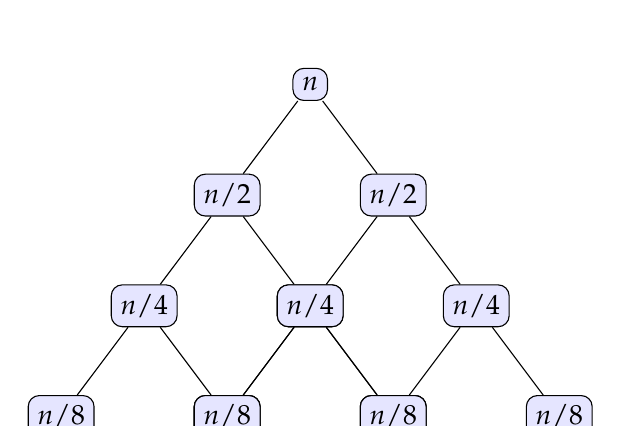
\begin{tikzpicture}[sibling distance=6em, level distance=4em, every node/.style={font=\footnotesize}]
\tikzstyle{every node}=[draw=black,rounded corners,fill=blue!10]
\node {\(n\)}
  child {node {\(n/2\)}
    child {node {\(n/4\)}
      child {node {\(n/8\)}}
      child {node {\(n/8\)}}
    }
    child {node {\(n/4\)}
      child {node {\(n/8\)}}
      child {node {\(n/8\)}}
    }
  }
  child {node {\(n/2\)}
    child {node {\(n/4\)}
      child {node {\(n/8\)}}
      child {node {\(n/8\)}}
    }
    child {node {\(n/4\)}
      child {node {\(n/8\)}}
      child {node {\(n/8\)}}
    }
  };
\end{tikzpicture}
\caption{Recursion Tree of Quick Sort in Best Case (Perfectly Balanced)}
\end{figure}

\paragraph{Observation:}
\begin{itemize}
  \item The recursion depth is \( \log n \) (base 2).
  \item Each level of the tree performs total work proportional to \( n \).
  \item Total time across all levels:
  \[
  n + n + n + \dots + n = n \log n
  \]
  \item Hence, the overall time complexity in the best/average case is:
  \[
  \boxed{T(n) = O(n \log n)}
  \]
\end{itemize}

\subsection*{\textbf{6. Insertion Sort}}
\begin{lstlisting}[language=C++, caption=Insertion Sort]
void insertionSort(vector<int>& arr) {
    for (int i = 1; i < arr.size(); i++) {
        int key = arr[i];
        int j = i - 1;
        while (j >= 0 && arr[j] > key) {
            arr[j + 1] = arr[j];
            j--;
        }
        arr[j + 1] = key;
    }
}
\end{lstlisting}

\subsection*{\textbf{6. Insertion Sort (Analysis)}}

\paragraph{Time Complexity Analysis:}

Insertion Sort builds the sorted array one element at a time. For each element, it is compared with all previous elements and shifted accordingly.

\begin{itemize}
  \item \textbf{Best Case:} The array is already sorted. Each element requires only one comparison:
  \[
  T(n) = \sum_{i=1}^{n-1} 1 = n - 1 \Rightarrow \boxed{O(n)}
  \]

  \item \textbf{Worst Case:} The array is reverse sorted. Every new element is compared with all previous elements and shifted:
  \[
  T(n) = \sum_{i=1}^{n-1} i = \frac{(n-1)n}{2} \Rightarrow \boxed{O(n^2)}
  \]

  \item \textbf{Average Case:} On average, each element is compared with half of the sorted part:
  \[
  T(n) = \sum_{i=1}^{n-1} \frac{i}{2} = \frac{1}{2} \cdot \frac{(n-1)n}{2} = \frac{n(n-1)}{4} \Rightarrow \boxed{O(n^2)}
  \]
\end{itemize}

\paragraph{Space Complexity:}

Insertion Sort is an in-place sorting algorithm.

\[
\boxed{\text{Space Complexity: } O(1)}
\]

\paragraph{Comparison Pattern (TikZ Visualization):}

\begin{figure}[H]
\centering
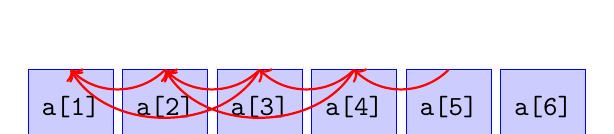
\begin{tikzpicture}[scale=1.2]
\foreach \i in {1,...,6} {
    \filldraw[blue!20, draw=blue] (\i, 0) rectangle (\i+0.9, 0.8);
    \node at (\i+0.45, 0.4) {\texttt{a[\i]}};
}

% Arrows showing comparison path
\draw[->, thick, red] (2.45, 0.8) to[bend left=45] (1.45, 0.8);
\draw[->, thick, red] (3.45, 0.8) to[bend left=45] (2.45, 0.8);
\draw[->, thick, red] (3.45, 0.8) to[bend left=60] (1.45, 0.8);
\draw[->, thick, red] (4.45, 0.8) to[bend left=45] (3.45, 0.8);
\draw[->, thick, red] (4.45, 0.8) to[bend left=60] (2.45, 0.8);
\draw[->, thick, red] (5.45, 0.8) to[bend left=45] (4.45, 0.8);
\end{tikzpicture}
\caption{Comparison pattern in Insertion Sort (Worst Case)}
\end{figure}

\paragraph{Summary:}

\begin{itemize}
  \item \textbf{Best Case:} \(\boxed{O(n)}\)
  \item \textbf{Average Case:} \(\boxed{O(n^2)}\)
  \item \textbf{Worst Case:} \(\boxed{O(n^2)}\)
  \item \textbf{Space Complexity:} \(\boxed{O(1)}\)
\end{itemize}


\subsection*{\textbf{7. Selection Sort}}
\begin{lstlisting}[language=C++, caption=Selection Sort]
void selectionSort(vector<int>& arr) {
    for (int i = 0; i < arr.size() - 1; i++) {
        int minIdx = i;
        for (int j = i + 1; j < arr.size(); j++) {
            if (arr[j] < arr[minIdx]) minIdx = j;
        }
        swap(arr[i], arr[minIdx]);
    }
}
\end{lstlisting}

\subsection*{\textbf{7. Selection Sort (Analysis)}}

\paragraph{Time Complexity Analysis:}

Selection Sort works by repeatedly finding the minimum element from the unsorted part and moving it to the sorted part. It always performs the same number of comparisons regardless of the initial order of the array.

\begin{itemize}
  \item \textbf{Best Case:} Array is already sorted. Still needs to compare all elements to find the minimum.
  \[
  T(n) = \sum_{i=0}^{n-2} (n - i - 1) = \frac{n(n - 1)}{2} \Rightarrow \boxed{O(n^2)}
  \]

  \item \textbf{Worst Case:} Array is in reverse order. Comparisons remain the same.
  \[
  T(n) = \sum_{i=0}^{n-2} (n - i - 1) = \frac{n(n - 1)}{2} \Rightarrow \boxed{O(n^2)}
  \]

  \item \textbf{Average Case:} Same number of comparisons as worst and best cases.
  \[
  \boxed{O(n^2)}
  \]
\end{itemize}

\paragraph{Swap Count:}

Unlike Insertion Sort, Selection Sort performs fewer swaps:
\[
\text{Maximum Swaps: } n - 1 \Rightarrow \boxed{O(n)}
\]

\paragraph{Space Complexity:}

Selection Sort is an in-place sorting algorithm and does not require extra space:
\[
\boxed{\text{Space Complexity: } O(1)}
\]

\paragraph{Comparison Pattern (TikZ Visualization):}

\begin{figure}[H]
\centering
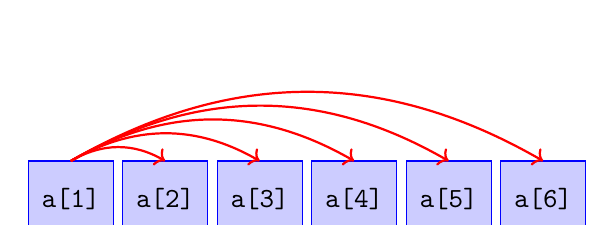
\begin{tikzpicture}[scale=1.2]
\foreach \i in {1,...,6} {
    \filldraw[blue!20, draw=blue] (\i, 0) rectangle (\i+0.9, 0.8);
    \node at (\i+0.45, 0.4) {\texttt{a[\i]}};
}

% Arrows showing selection comparison
\foreach \j in {2,...,6} {
  \draw[->, thick, red] (1.45, 0.8) to[bend left=30] (\j+0.45, 0.8);
}
\end{tikzpicture}
\caption{Selection of the minimum element in each iteration}
\end{figure}

\paragraph{Summary:}

\begin{itemize}
  \item \textbf{Best Case:} \(\boxed{O(n^2)}\)
  \item \textbf{Average Case:} \(\boxed{O(n^2)}\)
  \item \textbf{Worst Case:} \(\boxed{O(n^2)}\)
  \item \textbf{Swap Complexity:} \(\boxed{O(n)}\)
  \item \textbf{Space Complexity:} \(\boxed{O(1)}\)
\end{itemize}


\subsection*{\textbf{8. Heap Sort}}
\begin{lstlisting}[language=C++, caption=Heap Sort]
void heapify(vector<int>& arr, int n, int i) {
    int largest = i;
    int l = 2 * i + 1;
    int r = 2 * i + 2;
    if (l < n && arr[l] > arr[largest]){
        largest = l;
    }
    if (r < n && arr[r] > arr[largest]){
        largest = r;
    }
    if (largest != i) {
        swap(arr[i], arr[largest]);
        heapify(arr, n, largest);
    }
}
void heapSort(vector<int>& arr) {
    int n = arr.size();
    for (int i = n / 2 - 1; i >= 0; i--){
        heapify(arr, n, i);
    }
    for(int i = n - 1; i > 0; i--){
        swap(arr[0], arr[i]);
        heapify(arr, i, 0);
    }
}
\end{lstlisting}

\paragraph{Time Complexity Analysis (Max-Heap):}

\begin{itemize}
  \item \textbf{Heapify operation:} takes \( O(\log n) \).
  \item \textbf{Building heap:} \( O(n) \) (by applying heapify bottom-up).
  \item \textbf{Extracting max (n times):} \( n \cdot O(\log n) = O(n \log n) \).
\end{itemize}

\[
\boxed{\text{Overall Time Complexity (Max-Heap): } O(n \log n)}
\]

\paragraph{Space Complexity:}
Heap Sort is in-place:
\[
\boxed{O(1)}
\]

\paragraph{Tree Diagram (Max-Heap Representation):}

\begin{figure}[H]
\centering
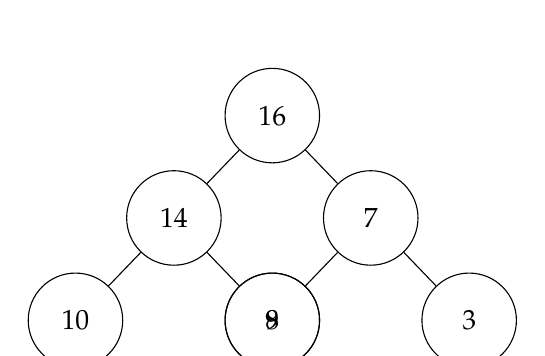
\begin{tikzpicture}[every node/.style={circle,draw,minimum size=1.2cm}, level distance=1.3cm, sibling distance=2.5cm]
\node {16}
  child {node {14}
    child {node {10}}
    child {node {8}}
  }
  child {node {7}
    child {node {9}}
    child {node {3}}
  };
\end{tikzpicture}
\caption{Max-Heap Tree Structure}
\end{figure}

\paragraph{Array Representation (Max-Heap):}

\[
\texttt{[16, 14, 7, 10, 8, 9, 3]}
\]

\paragraph{Tree Diagram (Min-Heap Representation):}

\begin{figure}[H]
\centering
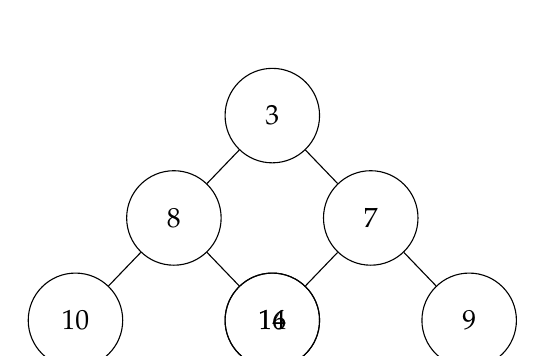
\begin{tikzpicture}[every node/.style={circle,draw,minimum size=1.2cm}, level distance=1.3cm, sibling distance=2.5cm]
\node {3}
  child {node {8}
    child {node {10}}
    child {node {14}}
  }
  child {node {7}
    child {node {16}}
    child {node {9}}
  };
\end{tikzpicture}
\caption{Min-Heap Tree Structure}
\end{figure}

\paragraph{Array Representation (Min-Heap):}

\[
\texttt{[3, 8, 7, 10, 14, 16, 9]}
\]

\paragraph{Time Complexity Analysis (Min-Heap):}
For a min-heap, if we sort in descending order, the time complexity is the same:
\begin{itemize}
  \item \textbf{Heapify:} \( O(\log n) \)
  \item \textbf{Build Heap:} \( O(n) \)
  \item \textbf{n Deletions:} \( O(n \log n) \)
\end{itemize}

\[
\boxed{\text{Overall Time Complexity (Min-Heap): } O(n \log n)}
\]

\paragraph{Summary:}
\begin{itemize}
  \item \textbf{Best Case:} \( O(n \log n) \)
  \item \textbf{Average Case:} \( O(n \log n) \)
  \item \textbf{Worst Case:} \( O(n \log n) \)
  \item \textbf{Space Complexity:} \( O(1) \)
  \item \textbf{Stable:} No
\end{itemize}


\subsection*{\textbf{9. Counting Sort}}
\begin{lstlisting}[language=C++, caption=Counting Sort (Non-negative Integers)]
void countingSort(vector<int>& arr) {
    if (arr.empty()){
        return;
    }
    int maxVal = *max_element(arr.begin(), arr.end());
    vector<int> count(maxVal + 1, 0);
    for (int num : arr){
        count[num]++;
    }
    int idx = 0;
    for (int i = 0; i <= maxVal; i++) {
        while (count[i]-- > 0) arr[idx++] = i;
    }
}
\end{lstlisting}

\paragraph{Time Complexity Analysis:}
Counting Sort assumes all input elements are non-negative integers and works by counting occurrences.

Let \( n \) be the number of elements and \( k \) be the range of input values.

\begin{itemize}
  \item \textbf{Counting frequency:} Takes \( O(n) \).
  \item \textbf{Populating sorted array:} Takes up to \( O(k) \) iterations.
\end{itemize}

\[
\boxed{\text{Time Complexity: } O(n + k)}
\]

\paragraph{Space Complexity:}
Extra space for the count array of size \( k + 1 \):
\[
\boxed{O(k)}
\]

\paragraph{Diagram Representation:}

\begin{figure}[H]
\centering
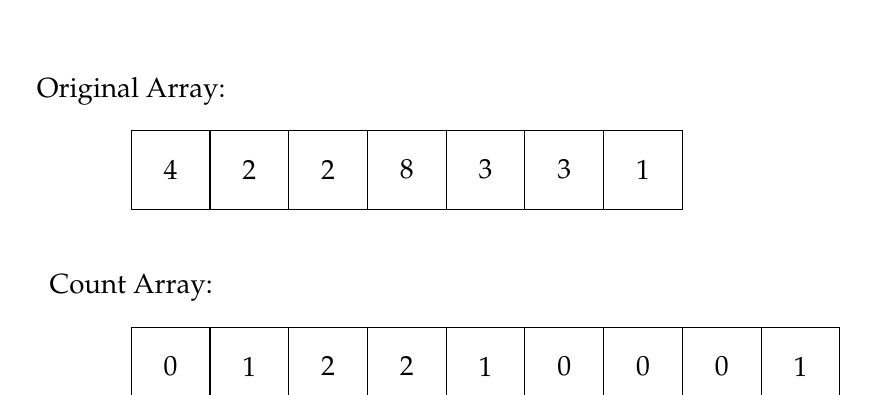
\begin{tikzpicture}[scale=1]
  % Original array
  \node at (0,0.5) {Original Array:};
  \foreach \x/\val in {0/4, 1/2, 2/2, 3/8, 4/3, 5/3, 6/1} {
    \draw (\x,0) rectangle (\x+1,-1);
    \node at (\x+0.5,-0.5) {\val};
  }

  % Count array
  \node at (0,-2) {Count Array:};
  \foreach \x/\val in {0/0, 1/1, 2/2, 3/2, 4/1, 5/0, 6/0, 7/0, 8/1} {
    \draw (\x,-2.5) rectangle (\x+1,-3.5);
    \node at (\x+0.5,-3) {\val};
  }
\end{tikzpicture}
\caption{Counting Sort Diagram: Frequency Count}
\end{figure}

\paragraph{Summary:}
\begin{itemize}
  \item \textbf{Best Case:} \( O(n + k) \)
  \item \textbf{Average Case:} \( O(n + k) \)
  \item \textbf{Worst Case:} \( O(n + k) \)
  \item \textbf{Space Complexity:} \( O(k) \)
  \item \textbf{Stable:} Yes
\end{itemize}

\subsection*{\textbf{10. Radix Sort}}
\begin{lstlisting}[language=C++, caption={Radix Sort (LSD, Non-negative Integers)}]
int getMax(vector<int>& arr) {
    return *max_element(arr.begin(), arr.end());
}
void countingSort(vector<int>& arr, int exp) {
    int n = arr.size();
    vector<int> output(n);
    vector<int> count(10, 0);
    for (int i = 0; i < n; i++) {
        count[(arr[i] / exp) % 10]++;
    }
    for (int i = 1; i < 10; i++) {
        count[i] += count[i - 1];
    }
    for (int i = n - 1; i >= 0; i--) {
        output[count[(arr[i] / exp) % 10] - 1] = arr[i];
        count[(arr[i] / exp) % 10]--;
    }
    for (int i = 0; i < n; i++) {
        arr[i] = output[i];
    }
}
void radixSort(vector<int>& arr) {
    if (arr.size() <= 1) return;
    int max = getMax(arr);
    for(int exp = 1; max / exp > 0; exp *= 10){
        countingSort(arr, exp);
    }
}
\end{lstlisting}

\paragraph{Time Complexity Analysis:}
Radix Sort processes each digit individually using Counting Sort as a stable subroutine.

Let:
\begin{itemize}
  \item \( n \) be the number of elements,
  \item \( k \) be the maximum value in the input,
  \item \( d \) be the number of digits in the maximum number (i.e., \( d = \log_{b} k \), where \( b \) is the base).
\end{itemize}

Each counting sort pass takes \( O(n + b) \) time and we do it for \( d \) digits:
\[
\boxed{\text{Time Complexity: } O(d(n + b)) = O(n \log k)}
\]

For decimal representation (\( b = 10 \)):
\[
\boxed{O(n \cdot \log_{10} k)}
\]

\paragraph{Space Complexity:}
Uses temporary arrays of size \( n \) and \( b \):
\[
\boxed{O(n + b)}
\]

\paragraph{Diagram Representation:}

\begin{figure}[H]
\centering
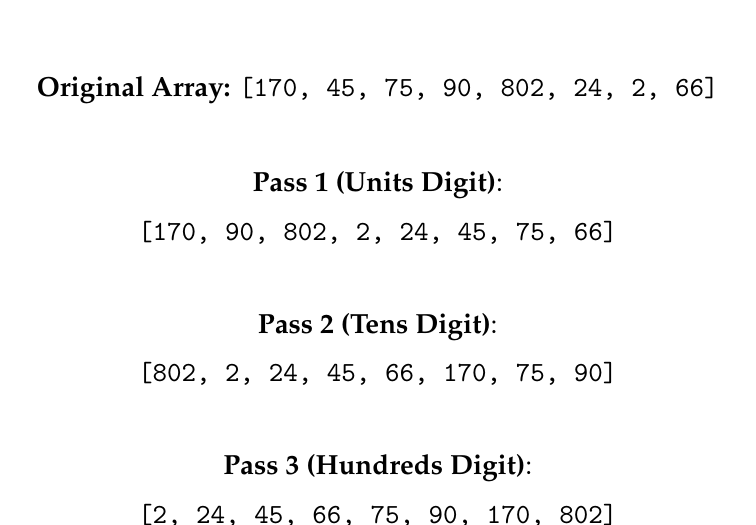
\begin{tikzpicture}[scale=1.2]
\node at (0,1.5) {\textbf{Original Array:} \texttt{[170, 45, 75, 90, 802, 24, 2, 66]}};

\node at (0,0.5) {\textbf{Pass 1 (Units Digit)}:};
\node at (0,0) {\texttt{[170, 90, 802, 2, 24, 45, 75, 66]}};

\node at (0,-1) {\textbf{Pass 2 (Tens Digit)}:};
\node at (0,-1.5) {\texttt{[802, 2, 24, 45, 66, 170, 75, 90]}};

\node at (0,-2.5) {\textbf{Pass 3 (Hundreds Digit)}:};
\node at (0,-3) {\texttt{[2, 24, 45, 66, 75, 90, 170, 802]}};
\end{tikzpicture}
\caption{Radix Sort Progression by Digit Position}
\end{figure}

\paragraph{Summary:}
\begin{itemize}
  \item \textbf{Best Case:} \( O(n \cdot \log_{b} k) \)
  \item \textbf{Average Case:} \( O(n \cdot \log_{b} k) \)
  \item \textbf{Worst Case:} \( O(n \cdot \log_{b} k) \)
  \item \textbf{Space Complexity:} \( O(n + b) \)
  \item \textbf{Stable:} Yes
\end{itemize}

\subsection*{\textbf{11. Bucket Sort}}
\begin{lstlisting}[language=C++, caption=Bucket Sort (Float numbers between 0 and 1)]
void bucketSort(vector<float>& arr) {
    int n = arr.size();
    vector<vector<float>> buckets(n);
    for (int i = 0; i < n; i++) {
        int idx = n * arr[i];
        buckets[idx].push_back(arr[i]);
    }
    for (int i = 0; i < n; i++){
        sort(buckets[i].begin(), buckets[i].end());
    }
    int idx = 0;
    for (int i = 0; i < n; i++) {
        for (float val : buckets[i]) {
            arr[idx++] = val;
        }
    }
}
\end{lstlisting}

\paragraph{Time Complexity Analysis:}
Bucket Sort distributes elements into buckets and sorts them individually.

Let:
\begin{itemize}
  \item \( n \) be the number of elements,
  \item \( k \) be the number of buckets (commonly \( k = n \)).
\end{itemize}

Assuming uniform distribution and insertion sort inside each bucket:

\begin{itemize}
  \item \textbf{Distribute into buckets:} \( O(n) \)
  \item \textbf{Sort each bucket:} Expected \( O(n) \) if elements are uniformly distributed
\end{itemize}

\[
\boxed{\text{Expected Time Complexity: } O(n)}
\]

\textbf{Worst-case:} When all elements fall into a single bucket, leading to:
\[
\boxed{O(n^2)}
\]

\paragraph{Space Complexity:}
Additional space for buckets:
\[
\boxed{O(n)}
\]

\paragraph{Diagram Representation:}

\begin{figure}[H]
\centering
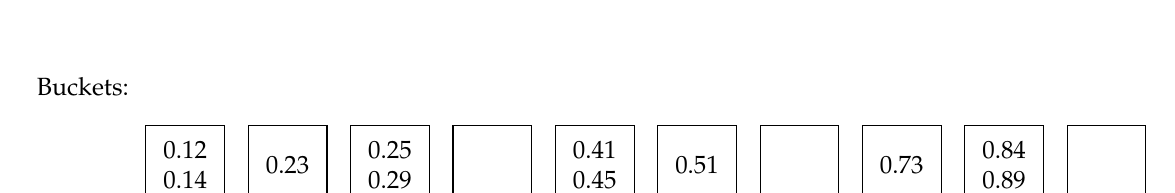
\begin{tikzpicture}[scale=1, every node/.style={font=\small}]
\node at (-0.8,0.5) {Buckets:};

% Buckets
\foreach \x/\val in {0/{0.12\\0.14}, 1/{0.23}, 2/{0.25\\0.29}, 3/{}, 4/{0.41\\0.45}, 5/{0.51}, 6/{}, 7/{0.73}, 8/{0.84\\0.89}, 9/{}} {
    \draw (\x*1.3,0) rectangle (\x*1.3+1, -1);
    \node[align=center] at (\x*1.3+0.5, -0.5) {\val};
}
\end{tikzpicture}
\caption{Bucket Sort Buckets with Sorted Values}
\end{figure}

\paragraph{Summary:}
\begin{itemize}
  \item \textbf{Best Case:} \( O(n) \)
  \item \textbf{Average Case:} \( O(n) \)
  \item \textbf{Worst Case:} \( O(n^2) \)
  \item \textbf{Space Complexity:} \( O(n) \)
  \item \textbf{Stable:} Depends on internal sort (e.g., insertion sort = stable)
\end{itemize}

\subsection*{\large \textbf{6. Highlighting Function Notations}}

We often express the dominating term of a function using color to emphasize its impact. For example, consider:
\[
\mathbf{f(n) = \textcolor{blue}{n^2} + 3n + 2}
\]
For large \( n \), the term \(\textcolor{blue}{n^2}\) dominates, hence:
\[
f(n) = \Theta(\textcolor{blue}{n^2})
\]
This shows that lower-order terms and constants are ignored in asymptotic analysis.
\chapter{Pointers in C++}

\section*{\Large \textbf{Pointers:}}
Pointers are variables that store the memory address of another variable. They are a powerful feature in C/C++ that allow direct memory access and manipulation. This chapter defines pointers, explains pointer-to-pointer, pointer arithmetic, and advanced pointer usage with examples, diagrams, and a comparison table.

\begin{figure}[h!]
  \centering
  \includegraphics[width=1\textwidth, height=10cm]{images/pointers.png}
  \caption{Pointer in C++}
  \label{fig:pointer_overview}
\end{figure}

\subsection*{\large \textbf{1. Definition and Explanation of Pointers}}

A \textbf{pointer} is a variable whose value is the address of another variable. For example, if we have an integer variable, its pointer will store the memory location where that integer is held.

\textbf{Key Points:}
\begin{itemize}[leftmargin=2em]
  \item Declaring a pointer: use the asterisk (\texttt{*}) before the pointer variable name.
  \item Dereferencing: the operator \texttt{*} is used to access the value at the memory address stored in the pointer.
  \item Address-of operator: the operator \texttt{\&} is used to get the memory address of a variable.
\end{itemize}

\subsection*{\large \textbf{2. Basic Pointer Usage in C++}}

\begin{lstlisting}[caption={Basic Pointer Example in C++}]
#include <iostream>
using namespace std;

int main() {
    int a = 42;
    int *ptr = &a;
    cout << "Value of a: " << a << endl;
    cout << "Address of a: " << &a << endl;
    cout << "Value stored in ptr (address of a): " << ptr << endl;
    cout << "Dereferenced ptr (value of a): " << *ptr << endl;
    return 0;
}
\end{lstlisting}

\subsection*{\large \textbf{3. Pointer to Pointer}}

A \textbf{pointer to pointer} stores the address of another pointer.

\begin{lstlisting}[caption={Pointer to Pointer in C++}]
#include <iostream>
using namespace std;

int main() {
    int a = 100;
    int *ptr = &a;
    int **pptr = &ptr;
    cout << "Value of a: " << a << endl;
    cout << "Address of a: " << &a << endl;
    cout << "ptr points to: " << ptr << endl;
    cout << "*ptr: " << *ptr << endl;
    cout << "pptr points to: " << pptr << endl;
    cout << "*pptr: " << *pptr << endl;
    cout << "**pptr: " << **pptr << endl;
    return 0;
}
\end{lstlisting}

\subsection*{\large \textbf{4. Pointer Arithmetic and Arrays}}

Pointer arithmetic is useful in array navigation. Adding 1 to a pointer makes it point to the next memory location of the pointed data type.

\begin{lstlisting}[caption={Pointer Arithmetic with Array in C++}]
#include <iostream>
using namespace std;

int main() {
    int arr[5] = {10, 20, 30, 40, 50};
    int *ptr = arr;
    cout << "Array elements using pointer arithmetic:" << endl;
    for (int i = 0; i < 5; i++) {
        cout << "Element " << i << ": " << *(ptr + i) << endl;
    }
    return 0;
}
\end{lstlisting}

\begin{figure}[H]
\centering
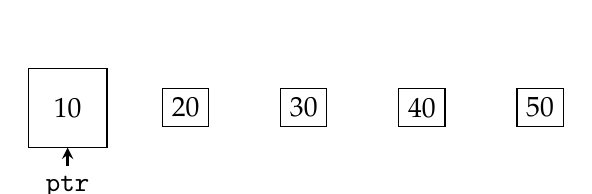
\begin{tikzpicture}[>=stealth, node distance=1.5cm]
    \node (a0) [draw, minimum width=1cm, minimum height=1cm] {10};
    \node (a1) [draw, right of=a0] {20};
    \node (a2) [draw, right of=a1] {30};
    \node (a3) [draw, right of=a2] {40};
    \node (a4) [draw, right of=a3] {50};

    \node (ptr) [below of=a0, yshift=0.5cm] {\texttt{ptr}};
    \draw[->, thick] (ptr.north) -- (a0.south);
\end{tikzpicture}
\caption{Pointer arithmetic: \texttt{ptr} points to \texttt{arr[0]}, \texttt{ptr+1} points to \texttt{arr[1]}, and so on.}
\end{figure}

\subsection*{\large \textbf{5. Table: Pointer Types and Use Cases}}

\begin{table}[H]
\centering
\begin{tabular}{|c|c|c|}
\hline
\textbf{Pointer Type} & \textbf{Declaration} & \textbf{Usage} \\
\hline
Single Pointer & \texttt{int *p;} & Holds address of an int \\
\hline
Double Pointer & \texttt{int **pp;} & Holds address of pointer to int \\
\hline
Null Pointer & \texttt{int *p = NULL;} & Indicates no address assigned \\
\hline
Void Pointer & \texttt{void *p;} & Generic pointer (typecast before use) \\
\hline
Function Pointer & \texttt{int (*fptr)(int);} & Points to a function \\
\hline
\end{tabular}
\caption{Common pointer types and their usage}
\end{table}

\section*{\Large \textbf{Summary}}
\begin{itemize}
  \item Pointers store memory addresses and enable dynamic memory access.
  \item They support arithmetic, point to arrays, and allow pointer-to-pointer usage.
  \item Advanced forms include void pointers, function pointers, and pointer arrays.
\end{itemize}
\chapter{Struct, Union and Enum}

\section*{Introduction}
C++ provides \textbf{struct}, \textbf{union}, and \textbf{enum} as user-defined data types. They allow grouping of variables under one name for efficient data management.

\section{Structure (\texttt{struct})}

\subsection*{Definition}
A structure is a collection of variables (of different types) grouped together under a single name.

\subsection*{Syntax}
\begin{lstlisting}[caption=Syntax of struct]
struct StructName {
    dataType member1;
    dataType member2;
    ...
};
\end{lstlisting}

\subsection*{Example}
\begin{lstlisting}[caption=C++ Code using struct]
#include <iostream>
using namespace std;

struct Student {
    int roll;
    float marks;
    char grade;
};

int main() {
    Student s1 = {101, 95.5, 'A'};
    cout << "Roll: " << s1.roll << "\n";
    cout << "Marks: " << s1.marks << "\n";
    cout << "Grade: " << s1.grade << "\n";
    return 0;
}
\end{lstlisting}

\subsection*{Accessing Members with Pointer}
\begin{lstlisting}[caption=Accessing struct members using pointer]
Student s = {102, 88.4, 'B'};
Student *ptr = &s;
cout << ptr->roll << "\n";
cout << ptr->marks << "\n";
cout << ptr->grade << "\n";
\end{lstlisting}

\subsection*{Memory Representation}
\begin{center}
\begin{tabular}{|c|c|c|c|}
\hline
Member & Type & Size (Bytes) & Offset \\
\hline
roll & int & 4 & 0 \\
marks & float & 4 & 4 \\
grade & char & 1 & 8 (may pad to 12) \\
\hline
\end{tabular}
\end{center}

\subsection*{Diagram}
\begin{figure}[H]
\centering
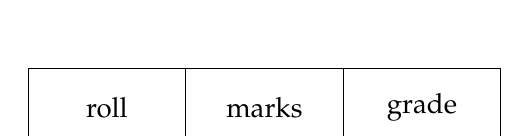
\begin{tikzpicture}[node distance=0cm,outer sep=0pt]
\node[draw, minimum width=2cm, minimum height=1cm] (a) {roll};
\node[draw, minimum width=2cm, minimum height=1cm, right=of a] (b) {marks};
\node[draw, minimum width=2cm, minimum height=1cm, right=of b] (c) {grade};
\end{tikzpicture}
\caption{Memory layout of struct Student}
\end{figure}

\subsection*{Advantages}
\begin{itemize}
  \item Group heterogeneous data types.
  \item Enhances code clarity and reusability.
  \item Useful in data modeling (e.g., records, databases).
\end{itemize}

\section{Union (\texttt{union})}

\subsection*{Definition}
A union allows storing different data types in the same memory location. Only one member can hold a value at a time.

\subsection*{Syntax}
\begin{lstlisting}[caption=Syntax of union]
union UnionName {
    dataType member1;
    dataType member2;
    ...
};
\end{lstlisting}

\subsection*{Example}
\begin{lstlisting}[caption=C++ Code using union]
#include <iostream>
using namespace std;

union Data {
    int i;
    float f;
};

int main() {
    Data d;
    d.i = 10;
    cout << "Integer: " << d.i << "\n";

    d.f = 3.14;
    cout << "Float: " << d.f << "\n";

    // Now d.i is likely corrupted
    cout << "Integer after float: " << d.i << "\n";
    return 0;
}
\end{lstlisting}

\subsection*{Memory Representation}
\begin{center}
\begin{tabular}{|c|c|c|}
\hline
Member & Type & Size (Bytes) \\
\hline
i & int & 4 \\
f & float & 4 \\
\hline
\end{tabular}
\end{center}
\vspace{0.2cm}
\textbf{Total Memory:} Max of all members (4 bytes here)

\begin{figure}[H]
\centering
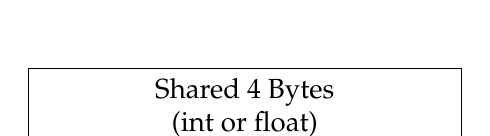
\begin{tikzpicture}
\draw (0,0) rectangle (5.5,1); % Wider box
\node at (2.75,0.5) {\parbox{5cm}{\centering Shared 4 Bytes\\(int or float)}};
\end{tikzpicture}
\caption{Union memory layout (shared memory)}
\end{figure}


\subsection*{Advantages}
\begin{itemize}
  \item Saves memory when only one member is used at a time.
  \item Useful in embedded systems and low-level programming.
\end{itemize}

\section{Enumeration (\texttt{enum})}

\subsection*{Definition}
An enum is a user-defined type consisting of a set of named integer constants.

\subsection*{Syntax}
\begin{lstlisting}[caption=Syntax of enum]
enum EnumName {
    CONSTANT1,
    CONSTANT2,
    ...
};
\end{lstlisting}

\subsection*{Example}
\begin{lstlisting}[caption=C++ Code using enum]
#include <iostream>
using namespace std;

enum Day {Mon, Tue, Wed, Thu, Fri, Sat, Sun};

int main() {
    Day d = Wed;
    cout << "Value of Wed: " << d << "\n";
    return 0;
}
\end{lstlisting}

\subsection*{Custom Values and Iteration}
\begin{lstlisting}[caption=Enum with custom values and loop]
enum Status {Pending=1, Approved=5, Rejected=10};

int main() {
    Status s = Approved;
    cout << "Status code: " << s << "\n";
    return 0;
}
\end{lstlisting}

\subsection*{Advantages}
\begin{itemize}
  \item Improves code readability.
  \item Restricts variable to valid set of values.
  \item Useful in state machines, switch cases.
\end{itemize}

\subsection*{Underlying Values}
\begin{verbatim}
By default: Mon = 0, Tue = 1, ..., Sun = 6
Custom: You can assign any value explicitly
\end{verbatim}

\begin{center}
\begin{tabular}{|c|c|}
\hline
Enum Constant & Value \\
\hline
Mon & 0 \\
Tue & 1 \\
Wed & 2 \\
Thu & 3 \\
Fri & 4 \\
Sat & 5 \\
Sun & 6 \\
\hline
\end{tabular}
\end{center}

\part{Linear Data Structures}
\chapter{Arrays}
% Content for Chapter 7

\section*{Introduction}
An \textbf{array} is a collection of elements, all of the same type, stored in contiguous memory locations. It allows for efficient access using indices. Arrays can be \textit{static} (fixed size) or \textit{dynamic} (resized at runtime). In C++, the STL \texttt{vector} provides a dynamic array implementation.

\begin{figure}[h!]
  \centering
  \includegraphics[width=0.5\textwidth, height=5cm]{images/array.png}
  \caption{Conceptual representation of an array in memory}
  \label{fig:array_concept}
\end{figure}

\section{Array Declarations and Syntax}

\subsection*{1D Array Declaration}
\textbf{Static (C/C++):}
\begin{lstlisting}[caption=Static 1D Array Declaration]
int arr[5]; // Declares an array of 5 integers
\end{lstlisting}

\textbf{Dynamic (C++ using pointers):}
\begin{lstlisting}[caption=Dynamic 1D Array Declaration using Pointers]
int* arr = new int[5]; // Allocates memory for 5 integers dynamically
\end{lstlisting}

\textbf{Using STL Vector (C++):}
\begin{lstlisting}[caption=1D Array using STL Vector]
#include <vector>
vector<int> arr(5); // Vector of size 5
\end{lstlisting}

\subsection*{2D Array Declaration}
\textbf{Static (C/C++):}
\begin{lstlisting}[caption=Static 2D Array Declaration]
int matrix[3][4]; // 3 rows and 4 columns
\end{lstlisting}

\textbf{Dynamic (C++ using pointers):}
\begin{lstlisting}[caption=Dynamic 2D Array Declaration using Pointers]
int** matrix = new int*[3];
for(int i = 0; i < 3; i++) {
    matrix[i] = new int[4];
}
\end{lstlisting}

\textbf{Using STL Vector (C++):}
\begin{lstlisting}[caption=2D Array using STL Vector]
#include <vector>
vector<vector<int>> matrix(3, vector<int>(4)); // 3x4 2D vector
\end{lstlisting}

\subsection*{3D Array Declaration (Using STL Vector)}
\begin{lstlisting}[caption=3D Array using STL Vector]
#include <vector>
vector<vector<vector<int>>> arr3D(
    2, vector<vector<int>>(
           3, vector<int>(4)));
// 2x3x4 3D vector
\end{lstlisting}

\section{Time and Space Complexity}
\subsection*{Time Complexity}
\begin{itemize}
  \item \textbf{Access:} \(O(1)\) - Direct access via index.
  \item \textbf{Search:} \(O(n)\) - Linear search in the worst case.
  \item \textbf{Insertion/Deletion at End:} \(O(1)\) - Amortized time.
  \item \textbf{Insertion/Deletion at Beginning or Middle:} \(O(n)\) - Requires shifting elements.
\end{itemize}

\subsection*{Space Complexity}
\begin{itemize}
  \item \textbf{Space:} \(O(n)\) - Where \(n\) is the number of elements in the array.
\end{itemize}

\section{Memory Allocation and Address Calculation}

\subsection*{Memory Allocation}
Arrays are stored in contiguous memory locations. For an array declared as \texttt{int arr[n];}, the memory layout is illustrated below:

\begin{center}
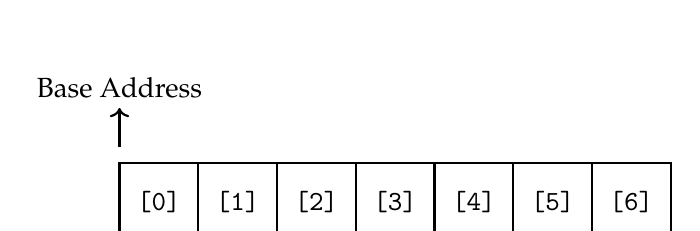
\begin{tikzpicture}[scale=1]
  \foreach \i in {0,1,2,3,4,5,6} {
    \draw[thick] (\i,0) rectangle (\i+1,1);
    \node at (\i+0.5,0.5) {\texttt{[\i]}};
  }
  \draw[->, thick] (0,1.2) -- (0,1.7) node[above]{Base Address};
\end{tikzpicture}
\end{center}

\subsection*{Address Calculation}
The address of the \(i\)th element is computed as:
\[
\text{Address of } arr[i] = \text{Base Address} + i \times \text{Size of each element}
\]

\subsection*{Indexing and Byte Addressing}
\textbf{0-Based Indexing:}
\[
\text{Address of } arr[i] = \text{Base Address} + i \times \text{Size}
\]
\textbf{1-Based Indexing:}
\[
\text{Address of } arr[i] = \text{Base Address} + (i-1) \times \text{Size}
\]

\section{Passing Arrays to Functions}
\subsection*{Example: Passing a 1D Array to a Function}
\begin{lstlisting}[style=cppstyle, caption=Passing Array to Function]
#include <bits/stdc++.h>
using namespace std;

void printArray(int arr[], int size) {
    for (int i = 0; i < size; ++i) {
        cout << arr[i] << " ";
    }
    cout << "\n";
}

int main() {
    int myArray[] = {10, 20, 30, 40, 50};
    int size = sizeof(myArray) / sizeof(myArray[0]);

    printArray(myArray, size);
    return 0;
}
\end{lstlisting}

\section{Two-Dimensional Arrays and Matrix Representation}
\subsection*{Row-Major Order}
The address of element \(A[i][j]\) is given by:
\[
\text{Address of } A[i][j] = B + [(i \cdot N) + j] \cdot w
\]
where \(B\) is the base address, \(N\) is the number of columns, and \(w\) is the size of each element.

\subsection*{Column-Major Order}
The address of element \(A[i][j]\) is:
\[
\text{Address of } A[i][j] = B + [(j \cdot M) + i] \cdot w
\]
where \(M\) is the number of rows.

\subsection*{Example: 2D Array in C++ (Row-Major Order)}
\begin{lstlisting}[style=cppstyle, caption=2D Array in Row-Major Order]
#include <bits/stdc++.h>
using namespace std;

int main() {
    int A[2][3] = {{1, 2, 3}, {4, 5, 6}};
    
    for (int i = 0; i < 2; i++) {
        for (int j = 0; j < 3; j++) {
            cout << A[i][j] << " ";
        }
        cout << endl;
    }
    return 0;
}
\end{lstlisting}

\section{Multidimensional Arrays}
Beyond 2D arrays, multidimensional arrays (such as 3D arrays) are used in applications like 3D graphics, simulations, and complex data representations.

\subsection*{Example: 3D Array (Using STL Vector in C++)}
\begin{lstlisting}[style=cppstyle, caption=3D Array Declaration using STL Vector]
#include <bits/stdc++.h>
using namespace std;

int main() {
    vector<vector<vector<int>>> arr3D(
        2, vector<vector<int>>(
               3, vector<int>(4, 0))); // 2x3x4 3D vector initialized with 0
    
    // Accessing an element:
    arr3D[0][1][2] = 42;
    
    cout << "Element at [0][1][2]: " << arr3D[0][1][2] << endl;
    return 0;
}
\end{lstlisting}

\section{Matrix Representation and Applications}
A matrix is typically represented as a 2D array and is used in:
\begin{itemize}
  \item Image representation (pixels)
  \item Graph adjacency matrices
  \item Dynamic programming tables
  \item Mathematical computations
\end{itemize}

\section{Drawbacks of Arrays}
Despite their efficiency, arrays have some limitations:
\begin{enumerate}
  \item \textbf{Fixed Size:} The size must be known at compile time for static arrays.
  \item \textbf{Memory Waste:} Overestimating size leads to unused memory, while underestimating can cause overflow.
  \item \textbf{Costly Insertions/Deletions:} Shifting elements results in \(O(n)\) time operations.
  \item \textbf{No Built-in Bound Checking:} Accessing out-of-bound indices causes undefined behavior.
  \item \textbf{Homogeneous Data:} Arrays store elements of the same type only.
  \item \textbf{Contiguous Memory Requirement:} Large blocks of contiguous memory might not be available in fragmented systems.
\end{enumerate}

\textbf{Solution:} Use STL containers like \texttt{vector} for dynamic arrays.

\section{Summary Table of Array Types and Syntax}
\begin{center}
\scriptsize % Or use \small if too tiny
\renewcommand{\arraystretch}{1.5}
\begin{tabular}{|l|p{3.2cm}|p{3.2cm}|p{4.5cm}|}
\hline
\textbf{Array Type} & \textbf{Declaration Syntax} & \textbf{Memory Allocation} & \textbf{Example / Notes} \\\hline

1D Static Array & \texttt{int arr[5];} & Stack, Contiguous & \texttt{int arr[5] = \{1, 2, 3, 4, 5\};} \\\hline

1D Dynamic Array & \texttt{int* arr = new int[5];} & Heap, Contiguous & Allocated at runtime using \texttt{new} \\\hline

2D Static Array & \texttt{int matrix[3][4];} & Stack, Row-major & 3 rows, 4 columns declared statically \\\hline

2D Dynamic Array & \texttt{int** matrix = new int*[3];} & Heap (row pointers), Contiguous rows & Allocate each row: \texttt{matrix[i] = new int[4];} \\\hline

STL 1D Vector & \texttt{vector<int> arr(5);} & Heap, Dynamic resizing & Uses STL; resizable, auto-managed memory \\\hline

STL 2D Vector & \texttt{vector<vector<int>> matrix;} & Heap, Nested Vectors & Allows jagged arrays; dynamic allocation \\\hline

STL 3D Vector & \texttt{vector<vector<..<int>.>} & Heap, Fully Dynamic & Example: \texttt{vector<vector<vector<int>>> arr3D(2, vector<vector<int>>(3, vector<int>(4)));} \\\hline
\end{tabular}
\captionof{table}{Summary of Array Types, Memory Allocation, and Syntax in C++}
\end{center}


\section{Additional Diagrams}
\subsection*{1D Array Memory Layout}
\begin{figure}[H]
\centering
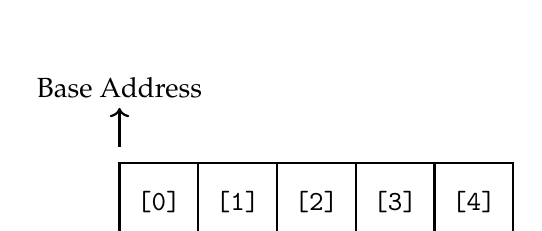
\begin{tikzpicture}[scale=1]
  \foreach \i in {0,1,2,3,4} {
    \draw[thick] (\i, 0) rectangle (\i+1, 1);
    \node at (\i+0.5,0.5) {\texttt{[\i]}};
  }
  \draw[->, thick] (0,1.2) -- (0,1.7) node[above]{Base Address};
\end{tikzpicture}
\caption{Memory layout of a 1D array with 5 elements.}
\end{figure}

\subsection*{2D Array Memory Layout (Row-Major)}
\begin{figure}[H]
\centering
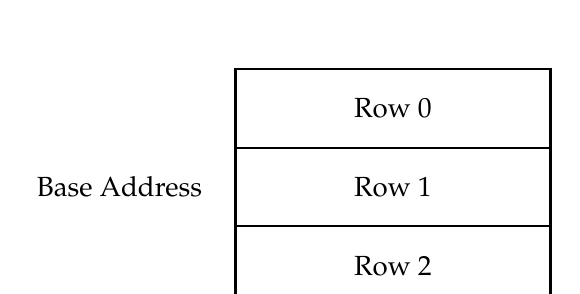
\begin{tikzpicture}[scale=1]
  \draw[thick] (0,0) rectangle (4,1) node[midway]{Row 0};
  \draw[thick] (0,-1) rectangle (4,0) node[midway]{Row 1};
  \draw[thick] (0,-2) rectangle (4,-1) node[midway]{Row 2};
  \node[anchor=east] at (-0.3,-0.5) {Base Address};
\end{tikzpicture}
\caption{Row-major layout of a 2D array (3 rows, 4 columns).}
\end{figure}


\section{Index Diagram and Table}

Consider a 1D array with 5 elements. The following table and diagram illustrate how array indices correspond to the stored elements.

\subsection*{Index Mapping Table}
\begin{table}[H]
\centering
\begin{tabular}{|c|c|}
\hline
\textbf{Index} & \textbf{Element (Label)} \\\hline
0 & \texttt{arr[0]} \\\hline
1 & \texttt{arr[1]} \\\hline
2 & \texttt{arr[2]} \\\hline
3 & \texttt{arr[3]} \\\hline
4 & \texttt{arr[4]} \\\hline
\end{tabular}
\caption{Mapping of indices to array elements for a 1D array}
\end{table}


\subsection*{1D Array Index Diagram}
\begin{figure}[H]
\centering
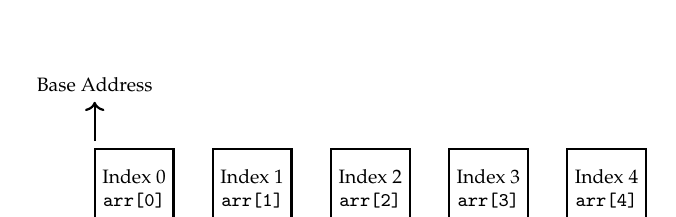
\begin{tikzpicture}[scale=1, every node/.style={font=\scriptsize}]
  % Draw boxes for each element
  \foreach \i in {0,1,2,3,4} {
    \draw[thick] (\i*1.5,0) rectangle (\i*1.5+1,1);
    \node at (\i*1.5+0.5,0.65) {Index \(\i\)};
    \node at (\i*1.5+0.5,0.35) {\texttt{arr[\i]}};
  }
  % Draw Base Address arrow
  \draw[->, thick] (0,1.1) -- (0,1.6) node[above]{Base Address};
\end{tikzpicture}

\caption{Index diagram for a 1D array of 5 elements}
\end{figure}



\chapter{Linked List}
% Content for Chapter 8

\section*{Introduction}
Linked lists are dynamic data structures in which nodes are linked together via pointers. They allow efficient insertions and deletions compared to static arrays. In this chapter, we cover three types of linked lists:
\begin{enumerate}
  \item \textbf{Singly Linked List}
  \item \textbf{Doubly Linked List}
  \item \textbf{Circular Linked List}
\end{enumerate}
Each type is explained in detail with corresponding C++ implementations, diagrams, and a summary of time and space complexities for common operations.

\section{Singly Linked List}

\subsection{Node Structure (Singly)}
\begin{lstlisting}[style=cppstyle, caption={Singly Linked List Node Structure in C++}]
struct Node {
    int data;
    Node* next;
    // Constructor for convenience
    Node(int val) : data(val), next(nullptr) {}
};
\end{lstlisting}

% --- Additional Theory for Singly Linked List ---
\textbf{Theory:} A singly linked list consists of nodes where each node holds data and a pointer to the next node. This design makes the list flexible in size, allowing nodes to be added or removed without reallocating or reorganizing the entire structure. However, because each node only points forward, traversing the list in reverse order is not straightforward without additional modifications.

\subsection{Operations on Singly Linked List}
\subsubsection{Insertion}
\begin{lstlisting}[style=cppstyle, caption={Insert at Front in Singly Linked List}]
void insertAtFront(Node*& head, int val) {
    Node* newNode = new Node(val);
    newNode->next = head;
    head = newNode;
}
\end{lstlisting}

\begin{lstlisting}[style=cppstyle, caption={Insert at End in Singly Linked List}]
void insertAtEnd(Node*& head, int val) {
    Node* newNode = new Node(val);
    if (!head) {
        head = newNode;
        return;
    }
    Node* temp = head;
    while (temp->next)
        temp = temp->next;
    temp->next = newNode;
}
\end{lstlisting}

\begin{lstlisting}[style=cppstyle, caption={Insert at Position in Singly Linked List}]
void insertAtPosition(Node*& head, int pos, int val) {
    if (pos == 0) {
        insertAtFront(head, val);
        return;
    }
    Node* newNode = new Node(val);
    Node* temp = head;
    for (int i = 0; temp != nullptr && i < pos - 1; i++)
        temp = temp->next;
    if (!temp) return; // Position out of bounds
    newNode->next = temp->next;
    temp->next = newNode;
}
\end{lstlisting}

% --- Additional Theory for Insertion in Singly Linked List ---
\textbf{Insertion Theory:} Insertion at the front of a singly linked list is very efficient (\(O(1)\)) because it simply involves updating the head pointer. Insertion at the end requires traversal of the entire list, resulting in \(O(n)\) time complexity. When inserting at a given position, the list must be traversed until that position is reached, making it \(O(n)\) as well. These operations illustrate the trade-off between flexibility and direct access in linked lists.

\subsubsection{Deletion}
\begin{lstlisting}[style=cppstyle, caption={Delete from Front in Singly Linked List}]
void deleteFromFront(Node*& head) {
    if (!head) return;
    Node* temp = head;
    head = head->next;
    delete temp;
}
\end{lstlisting}

\begin{lstlisting}[style=cppstyle, caption={Delete from End in Singly Linked List}]
void deleteFromEnd(Node*& head) {
    if (!head) return;
    if (!head->next) {
        delete head;
        head = nullptr;
        return;
    }
    Node* temp = head;
    while (temp->next && temp->next->next)
        temp = temp->next;
    delete temp->next;
    temp->next = nullptr;
}
\end{lstlisting}

\begin{lstlisting}[style=cppstyle, caption={Delete from Position in Singly Linked List}]
void deleteAtPosition(Node*& head, int pos) {
    if (!head) return;
    if (pos == 0) {
        deleteFromFront(head);
        return;
    }
    Node* temp = head;
    for (int i = 0; temp != nullptr && i < pos - 1; i++)
        temp = temp->next;
    if (!temp || !temp->next) return; // Position out of bounds
    Node* delNode = temp->next;
    temp->next = delNode->next;
    delete delNode;
}
\end{lstlisting}

% --- Additional Theory for Deletion in Singly Linked List ---
\textbf{Deletion Theory:} Deletion operations in a singly linked list are efficient if the node to be deleted is known (\(O(1)\)). However, if a search is needed to find the node, the operation becomes \(O(n)\). The simplicity of pointer adjustments in deletion is a key advantage over array-based structures.

\subsubsection{Search}
\begin{lstlisting}[style=cppstyle, caption={Search in Singly Linked List}]
int search(Node* head, int key) {
    int index = 0;
    while (head) {
        if (head->data == key)
            return index;
        head = head->next;
        index++;
    }
    return -1; // Not found
}
\end{lstlisting}

% --- Additional Theory for Search in Singly Linked List ---
\textbf{Search Theory:} Since singly linked lists are sequential, searching for an element requires traversing the list from the head until the element is found, leading to \(O(n)\) time complexity. This is less efficient compared to direct indexing in arrays but is acceptable given the dynamic nature of linked lists.

\subsection{Diagram: Singly Linked List}
\begin{center}
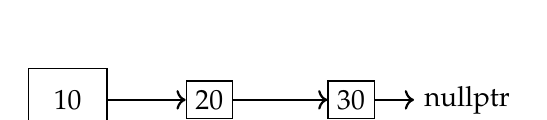
\begin{tikzpicture}[node distance=1.8cm, auto]
  \node (n1) [draw, rectangle, minimum width=1cm, minimum height=0.8cm] {10};
  \node (n2) [draw, rectangle, right of=n1] {20};
  \node (n3) [draw, rectangle, right of=n2] {30};
  \draw[->, thick] (n1.east) -- (n2.west);
  \draw[->, thick] (n2.east) -- (n3.west);
  \draw[->, thick] (n3.east) -- ++(0.5,0) node[right]{nullptr};
\end{tikzpicture}
\captionof{figure}{Singly Linked List Diagram}
\end{center}

\newpage

\section{Doubly Linked List}

\subsection{Node Structure (Doubly)}
\begin{lstlisting}[style=cppstyle, caption={Doubly Linked List Node Structure in C++}]
struct DNode {
    int data;
    DNode* next;
    DNode* prev;
    DNode(int val) : data(val), next(nullptr), prev(nullptr) {}
};
\end{lstlisting}

\subsection{Operations on Doubly Linked List}
\subsubsection{Insertion}
\begin{lstlisting}[style=cppstyle, caption={Insert at Front in Doubly Linked List}]
void insertAtFront(DNode*& head, int val) {
    DNode* newNode = new DNode(val);
    newNode->next = head;
    if (head)
        head->prev = newNode;
    head = newNode;
}
\end{lstlisting}

\begin{lstlisting}[style=cppstyle, caption={Insert at End in Doubly Linked List}]
void insertAtEnd(DNode*& head, int val) {
    DNode* newNode = new DNode(val);
    if (!head) {
        head = newNode;
        return;
    }
    DNode* temp = head;
    while (temp->next)
        temp = temp->next;
    temp->next = newNode;
    newNode->prev = temp;
}
\end{lstlisting}

% --- Additional Theory for Doubly Linked List Insertion ---
\textbf{Theory:} Doubly linked lists maintain two pointers in each node, which allows traversal in both directions. This feature simplifies certain operations like deletion and backward traversal but requires additional memory for the extra pointer.

\subsubsection{Deletion}
\begin{lstlisting}[style=cppstyle, caption={Delete from Front in Doubly Linked List}]
void deleteFromFront(DNode*& head) {
    if (!head) return;
    DNode* temp = head;
    head = head->next;
    if (head)
        head->prev = nullptr;
    delete temp;
}
\end{lstlisting}

\begin{lstlisting}[style=cppstyle, caption={Delete from End in Doubly Linked List}]
void deleteFromEnd(DNode*& head) {
    if (!head) return;
    if (!head->next) {
        delete head;
        head = nullptr;
        return;
    }
    DNode* temp = head;
    while (temp->next)
        temp = temp->next;
    temp->prev->next = nullptr;
    delete temp;
}
\end{lstlisting}

\begin{lstlisting}[style=cppstyle, caption={Search in Doubly Linked List}]
int search(DNode* head, int key) {
    int index = 0;
    while (head) {
        if (head->data == key)
            return index;
        head = head->next;
        index++;
    }
    return -1;
}
\end{lstlisting}

\subsection{Diagram: Doubly Linked List}
\begin{center}
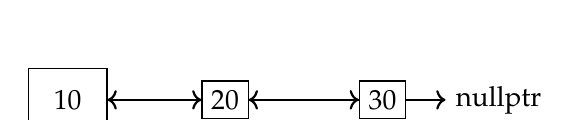
\begin{tikzpicture}[node distance=2cm, auto]
  \node (d1) [draw, rectangle, minimum width=1cm, minimum height=0.8cm] {10};
  \node (d2) [draw, rectangle, right of=d1] {20};
  \node (d3) [draw, rectangle, right of=d2] {30};
  \draw[->, thick] (d1.east) -- (d2.west);
  \draw[->, thick] (d2.west) -- (d1.east);
  \draw[->, thick] (d2.east) -- (d3.west);
  \draw[->, thick] (d3.west) -- (d2.east);
  \draw[->, thick] (d3.east) -- ++(0.5,0) node[right]{nullptr};
\end{tikzpicture}
\captionof{figure}{Doubly Linked List Diagram}
\end{center}

\newpage

\section{Circular Linked List}

\subsection{Node Structure (Circular)}
\begin{lstlisting}[style=cppstyle, caption={Circular Linked List Node Structure in C++}]
struct CNode {
    int data;
    CNode* next;
    CNode(int val) : data(val), next(nullptr) {}
};
\end{lstlisting}

\subsection{Operations on Circular Linked List}
\subsubsection{Insertion}
\begin{lstlisting}[style=cppstyle, caption={Insert in Circular Linked List}]
void insertCircular(CNode*& head, int val) {
    CNode* newNode = new CNode(val);
    if (!head) {
        head = newNode;
        newNode->next = head;
        return;
    }
    CNode* temp = head;
    while (temp->next != head)
        temp = temp->next;
    temp->next = newNode;
    newNode->next = head;
}
\end{lstlisting}

\subsubsection{Deletion}
\begin{lstlisting}[style=cppstyle, caption={Delete Node in Circular Linked List}]
void deleteCircular(CNode*& head, int key) {
    if (!head) return;
    // If head is to be deleted
    if (head->data == key) {
        if (head->next == head) { // Only one node exists
            delete head;
            head = nullptr;
            return;
        }
        // Find last node to update its next pointer
        CNode* temp = head;
        while (temp->next != head)
            temp = temp->next;
        CNode* del = head;
        head = head->next;
        temp->next = head;
        delete del;
        return;
    }
    // Delete node other than head
    CNode* curr = head;
    while (curr->next != head && curr->next->data != key)
        curr = curr->next;
    if (curr->next->data == key) {
        CNode* del = curr->next;
        curr->next = del->next;
        delete del;
    }
}
\end{lstlisting}

\subsubsection{Search}
\begin{lstlisting}[style=cppstyle, caption={Search in Circular Linked List}]
int searchCircular(CNode* head, int key) {
    if (!head) return -1;
    int index = 0;
    CNode* temp = head;
    do {
        if (temp->data == key)
            return index;
        temp = temp->next;
        index++;
    } while (temp != head);
    return -1;
}
\end{lstlisting}

\subsection{Diagram: Circular Linked List}
\begin{center}
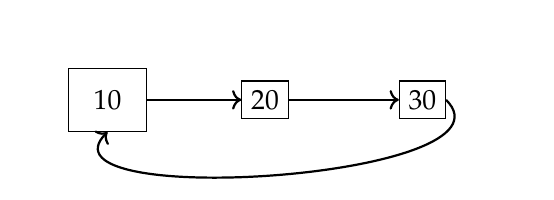
\begin{tikzpicture}[node distance=2cm, auto]
  \node (c1) [draw, rectangle, minimum width=1cm, minimum height=0.8cm] {10};
  \node (c2) [draw, rectangle, right of=c1] {20};
  \node (c3) [draw, rectangle, right of=c2] {30};
  \draw[->, thick] (c1.east) -- (c2.west);
  \draw[->, thick] (c2.east) -- (c3.west);
  \draw[->, thick] (c3.east) .. controls +(1,-1) and +(-1,-1) .. (c1.south);
\end{tikzpicture}
\captionof{figure}{Circular Linked List Diagram}
\end{center}

\section{Complexity Analysis for Linked List Operations}
\begin{table}[H]
\centering
\renewcommand{\arraystretch}{1.5}
\begin{tabular}{|l|c|c|}
\hline
\textbf{Operation} & \textbf{Time Complexity} & \textbf{Space Complexity} \\ \hline
Access             & \(O(n)\)  & \(O(n)\) (node overhead) \\ \hline
Search             & \(O(n)\)  & \(O(1)\) \\ \hline
Insertion (given pointer) & \(O(1)\) & \(O(1)\) \\ \hline
Insertion (search required) & \(O(n)\) & \(O(1)\) \\ \hline
Deletion (given pointer) & \(O(1)\) & \(O(1)\) \\ \hline
Deletion (search required) & \(O(n)\) & \(O(1)\) \\ \hline
\end{tabular}
\caption{Time and Space Complexity of Linked List Operations}
\end{table}

\section{Syntax Summary for Linked List Node Structures}
\begin{center}
\renewcommand{\arraystretch}{1.5}
\begin{tabular}{|l|l|}
\hline
\textbf{Type} & \textbf{Node Structure Syntax} \\\hline
Singly Linked List & \texttt{struct Node \{ int data; Node* next; \}} \\\hline
Doubly Linked List & \texttt{struct DNode \{ int data; DNode* next; DNode* prev; \}} \\\hline
Circular Linked List & \texttt{struct CNode \{ int data; CNode* next; \}} \\\hline
\end{tabular}
\captionof{table}{Node Structure Syntax for Different Linked Lists}
\end{center}

\section{Additional Theoretical Concepts}

\subsection{Singly Linked List Theory}
Singly linked lists are one of the simplest forms of linked lists. They are ideal for implementations where only forward traversal is needed. Their simplicity, however, comes at a cost: operations like finding the previous node require traversing the list from the head, which can be inefficient. They are best used in scenarios where memory reallocation is frequent and operations mostly involve adding or removing nodes at the head.

\subsection{Doubly Linked List Theory}
Doubly linked lists enhance singly linked lists by providing backward pointers. This allows efficient bidirectional traversal, which simplifies operations like deletion from the end or inserting before a given node. However, this comes at the cost of additional memory for the extra pointer, and the operations are slightly more complex because both pointers must be updated during insertions and deletions.

\subsection{Circular Linked List Theory}
Circular linked lists differ from the other types in that the last node points back to the first node, forming a continuous loop. This structure is useful for applications where the list needs to be traversed cyclically (e.g., round-robin scheduling). They eliminate the need for null checks at the end of the list, but careful handling is required during insertion and deletion to avoid infinite loops.

\subsection{Memory Management and Pointer Usage}
Linked lists dynamically allocate memory for each node, which means memory is used only as needed. However, the overhead of storing pointers in each node can be significant compared to array elements. In systems with limited memory, the trade-off between flexibility and memory overhead must be considered. Garbage collection (in languages that support it) or manual memory management in C++ is essential to avoid memory leaks.

\section{Conclusion}
Linked lists are versatile and powerful dynamic data structures that provide efficient insertion and deletion operations. Each type—singly, doubly, and circular—has its own advantages and trade-offs. Singly linked lists are simple and efficient for forward traversal; doubly linked lists allow for bidirectional movement; and circular linked lists facilitate continuous looping without explicit null termination. Understanding the underlying theory, along with the syntax and complexity of various operations, is crucial for designing efficient data structures and algorithms.

\vspace{1em}
This chapter provides both practical C++ implementations and theoretical insights to help you master linked list concepts.

\chapter{Stack}

\section{Introduction}
A \textbf{stack} is a fundamental abstract data type that operates on the Last In First Out (LIFO) principle. In other words, the last element added to the stack is the first one to be removed. Stacks are widely used in various computing applications, including expression evaluation, recursion management, and backtracking algorithms.

\section{Definition and Theoretical Background}
A stack supports the following primary operations:
\begin{itemize}
    \item \textbf{Push}: Add an element to the top of the stack.
    \item \textbf{Pop}: Remove the element from the top of the stack.
    \item \textbf{Top/Peek}: Retrieve the top element without removing it.
    \item \textbf{IsEmpty}: Check whether the stack is empty.
\end{itemize}

Formally, a stack \( S \) can be defined as a tuple \( (D, P) \), where:
\begin{itemize}
    \item \( D \) is a finite set of data elements.
    \item \( P \) is a pointer or index indicating the top element in the stack.
\end{itemize}

The operations are defined as:
\begin{itemize}
    \item \textbf{Push}: For a stack \( S = (D, P) \), pushing an element \( x \) transforms it into \( S' = (D \cup \{x\}, x) \). The new element becomes the top element.
    \item \textbf{Pop}: Removing the top element \( x \) from \( S \) results in a new stack \( S' = (D \setminus \{x\}, y) \), where \( y \) is now the top element.
    \item \textbf{Top/Peek}: This operation retrieves \( x \) (the current top element) without modifying the stack.
    \item \textbf{IsEmpty}: A boolean function that returns true if no elements are in \( D \) (i.e., \( P \) is undefined or negative).
\end{itemize}

\subsection{Additional Theoretical Considerations}
There are two common ways to implement a stack:
\begin{itemize}
    \item \textbf{Array-based Implementation}: Uses a fixed-size array to store elements. It is simple and fast but has a size limitation.
    \item \textbf{Linked List Implementation}: Uses nodes where each node points to the next element. It can grow dynamically, although it may incur extra memory overhead.
\end{itemize}

Understanding these two implementations is essential because each has its own performance characteristics and trade-offs in terms of time and space complexity.

\section{Diagrams of Stack Operations}

\subsection{Overall Stack Structure}
The following diagram shows a simple stack with three elements. The top element is at the uppermost position:
\begin{center}
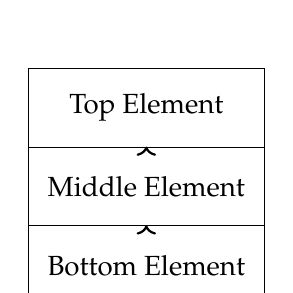
\begin{tikzpicture}[node distance=1cm]
    % Nodes representing stack elements
    \node (top) [draw, rectangle, minimum width=3cm, minimum height=1cm] {Top Element};
    \node (middle) [draw, rectangle, below of=top, minimum width=3cm, minimum height=1cm] {Middle Element};
    \node (bottom) [draw, rectangle, below of=middle, minimum width=3cm, minimum height=1cm] {Bottom Element};

    % Arrows showing order
    \draw[->, thick] (top.south) -- (middle.north);
    \draw[->, thick] (middle.south) -- (bottom.north);
\end{tikzpicture}
\end{center}

\subsection{Push Operation Diagram}
The diagram below illustrates a push operation. A new element is inserted and becomes the new top:
\begin{center}
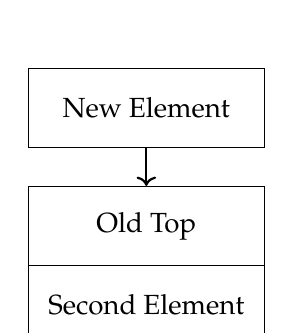
\begin{tikzpicture}[node distance=1cm]
    % Before push
    \node (oldtop) [draw, rectangle, minimum width=3cm, minimum height=1cm] {Old Top};
    \node (below) [draw, rectangle, below of=oldtop, minimum width=3cm, minimum height=1cm] {Second Element};

    % New element coming in
    \node (newelem) [draw, rectangle, minimum width=3cm, minimum height=1cm, above of=oldtop, node distance=1.5cm] {New Element};

    % Arrows to indicate push
    \draw[->, thick] (newelem.south) -- (oldtop.north);
\end{tikzpicture}
\end{center}

\subsection{Pop Operation Diagram}
The following diagram shows the pop operation, where the top element is removed:
\begin{center}
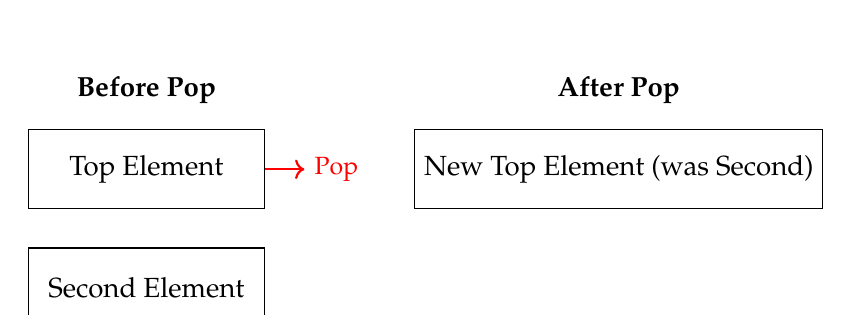
\begin{tikzpicture}[node distance=1cm]

% --- Stack BEFORE pop ---
\node at (0, 2.5) {\textbf{Before Pop}};
\node (before_top) [draw, rectangle, minimum width=3cm, minimum height=1cm] at (0,1.5) {Top Element};
\node (before_second) [draw, rectangle, minimum width=3cm, minimum height=1cm] at (0,0) {Second Element};
\draw[->, thick, red] (before_top.east) -- ++(0.5,0) node[right]{\small Pop};

% --- Stack AFTER pop ---
\node at (6, 2.5) {\textbf{After Pop}};
\node (after_top) [draw, rectangle, minimum width=3cm, minimum height=1cm] at (6,1.5) {New Top Element (was Second)};

\end{tikzpicture}
\end{center}


\section{C++ Implementation of a Stack}
Below is an extended implementation of a stack using an array in C++ with additional inline comments for clarity.

\begin{lstlisting}[caption={C++ implementation of a Stack using an array}]
#include <bits/stdc++.h>
#define MAX 100

class Stack {
private:
    int arr[MAX]; // Array to store stack elements
    int top;      // Index of the top element
public:
    // Constructor initializes top to -1 indicating an empty stack
    Stack() : top(-1) {}

    // Check if the stack is empty
    bool isEmpty() {
        return (top < 0);
    }
    // Push an element onto the stack
    bool push(int x) {
        if(top >= (MAX - 1)) {
            cout << "Stack Overflow" << "\n";
            return false;
        } else {
            arr[++top] = x;
            return true;
        }
    }
    // Pop an element from the stack
    int pop() {
        if(isEmpty()){
            cout << "Stack Underflow" << "\n";
            return -1;
        } else {
            int x = arr[top--];
            return x;
        }
    }
    // Peek at the top element without removing it
    int peek() {
        if(isEmpty()){
            cout << "Stack is Empty" << "\n";
            return -1;
        } else {
            return arr[top];
        }
    }
};
int main() {
    Stack s;
    // Example operations on the stack
    s.push(10);   // Stack: [10]
    s.push(20);   // Stack: [10, 20]
    s.push(30);   // Stack: [10, 20, 30]
    cout << "Top element is " << s.peek() << "\n"; // Should print 30
    cout << "Popped element is " << s.pop() << "\n"; // Removes 30
    cout << "New top element is " << s.peek() << "\n"; // Should print 20

    return 0;
}
\end{lstlisting}

\section{Example Scenario in Detail}
Consider the following sequence of operations on an initially empty stack:
\begin{enumerate}
    \item \textbf{Push} 5 onto the stack. \\
          \textbf{Stack state}: [5] (5 becomes the top element)
    \item \textbf{Push} 10 onto the stack. \\
          \textbf{Stack state}: [5, 10] (10 is now at the top)
    \item \textbf{Push} 15 onto the stack. \\
          \textbf{Stack state}: [5, 10, 15] (15 becomes the new top)
    \item \textbf{Pop} the top element. \\
          \textbf{Stack state}: [5, 10] (15 is removed; 10 becomes the top)
\end{enumerate}

The above scenario is illustrated in the diagrams provided earlier. When a new element is pushed, it becomes the new top, and when an element is popped, the previous element becomes the top.

\section{Infix, Postfix, and Prefix Conversion}

Expressions can be written in three common forms:
\begin{itemize}
    \item \textbf{Infix:} The operator is written between the operands (e.g., \texttt{A + B}).
    \item \textbf{Postfix (Reverse Polish Notation):} The operator follows the operands (e.g., \texttt{A B +}).
    \item \textbf{Prefix (Polish Notation):} The operator precedes the operands (e.g., \texttt{+ A B}).
\end{itemize}

\subsection{Theory and Conversion Algorithms}
To convert an infix expression to postfix, follow these steps:
\begin{enumerate}
    \item Scan the infix expression from left to right.
    \item Use a stack to store operators and an output string for the result.
    \item When an operand (letter or number) is encountered, append it to the output.
    \item When an operator is encountered, pop from the stack to the output until either the stack is empty or the operator at the top of the stack has lower precedence than the current operator. Then, push the current operator onto the stack.
    \item When a left parenthesis \texttt{(} is encountered, push it onto the stack.
    \item When a right parenthesis \texttt{)} is encountered, pop from the stack to the output until a left parenthesis is encountered; then discard the pair of parentheses.
    \item After processing the entire expression, pop any remaining operators from the stack to the output.
\end{enumerate}

For \textbf{infix to prefix conversion}, a common method is:
\begin{itemize}
    \item Reverse the infix expression.
    \item Swap every \texttt{(} with \texttt{)} and vice-versa.
    \item Convert the modified expression to postfix.
    \item Reverse the resulting postfix expression to obtain the prefix expression.
\end{itemize}

\subsection{Extended C++ Implementation}

Below is an extended C++ code that implements both infix-to-postfix and infix-to-prefix conversion. Notice the use of helper functions to reverse strings and swap parentheses.

\begin{lstlisting}[language=C++, caption={Extended C++ Code for Infix, Postfix, and Prefix Conversion}]
#include <bits/stdc++.h>

using namespace std;

// Function to return precedence of operators
int precedence(char op) {
    if(op == '+' || op == '-') return 1;
    if(op == '*' || op == '/') return 2;
    return 0;
}
// Infix to Postfix conversion
string infixToPostfix(const string &infix) {
    string postfix;
    stack<char> s;
    for (char c : infix) {
        // If the character is an operand, append it to output
        if(isalnum(c))
            postfix += c;
        // If '(' encountered, push to stack
        else if(c == '(')
            s.push(c);
        // If ')' encountered, pop until '('
        else if(c == ')') {
            while(!s.empty() && s.top() != '(') {
                postfix += s.top();
                s.pop();
            }
            if(!s.empty())
                s.pop(); // pop '('
        }
        // If operator encountered
        else {
            while(!s.empty() && precedence(c) <= precedence(s.top())) {
                postfix += s.top();
                s.pop();
            }
            s.push(c);
        }
    }
    // Pop remaining operators
    while(!s.empty()) {
        postfix += s.top();
        s.pop();
    }
    return postfix;
}
// Utility function to reverse a string
string reverseString(string s) {
    reverse(s.begin(), s.end());
    return s;
}
// Swap parentheses in a string
string swapParentheses(string s) {
    for (char &c : s) {
        if(c == '(') c = ')';
        else if(c == ')') c = '(';
    }
    return s;
}

// Infix to Prefix conversion using reverse-process method
string infixToPrefix(string infix) {
    // Reverse the infix expression and swap parentheses
    string rev = reverseString(infix);
    rev = swapParentheses(rev);
    // Convert reversed expression to postfix
    string revPostfix = infixToPostfix(rev);
    // Reverse the postfix expression to get prefix
    string prefix = reverseString(revPostfix);
    return prefix;
}

int main() {
    // Example 1
    string infix1 = "((A+B)*C)-(D/E)";
    cout << "Infix 1: " << infix1 << endl;
    cout << "Postfix 1: " << infixToPostfix(infix1) << endl;
    cout << "Prefix 1: " << infixToPrefix(infix1) << endl << endl;
    
    // Example 2
    string infix2 = "A*(B+C)/D";
    cout << "Infix 2: " << infix2 << endl;
    cout << "Postfix 2: " << infixToPostfix(infix2) << endl;
    cout << "Prefix 2: " << infixToPrefix(infix2) << endl;
    
    return 0;
}
\end{lstlisting}

\subsection{Expression Tree Diagrams}

The following diagrams represent the expression trees for the given expressions. These trees help visualize how the expressions are structured and how different traversals yield the infix, postfix, and prefix notations.

\subsubsection*{Example 1: \( ((A+B)*C)-(D/E) \)}

\textbf{Expression Tree:}

\begin{center}
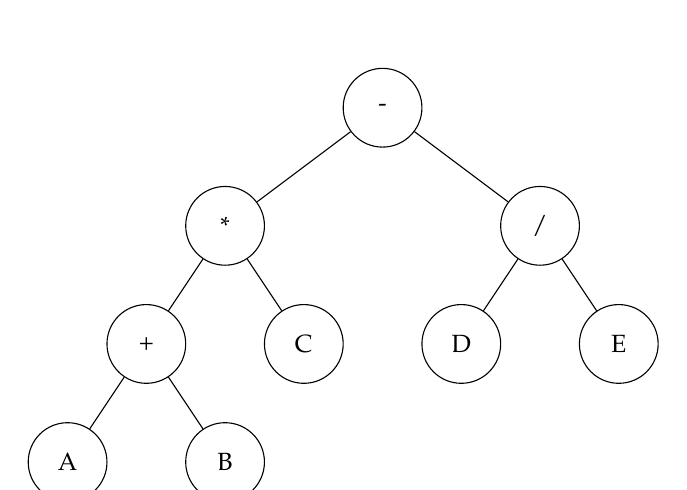
\begin{tikzpicture}[level distance=1.5cm,
  level 1/.style={sibling distance=4cm},
  level 2/.style={sibling distance=2cm},
  every node/.style={draw, circle, minimum size=1cm, font=\small}]
  \node { - }
    child { node { * }
      child { node { + }
        child { node { A } }
        child { node { B } }
      }
      child { node { C } }
    }
    child { node { / }
      child { node { D } }
      child { node { E } }
    };
\end{tikzpicture}
\end{center}

\textbf{Traversals:}
\begin{itemize}
    \item \textbf{Inorder (Infix):} \( ((A+B)*C)-(D/E) \)
    \item \textbf{Postorder (Postfix):} \( A\,B\,+\,C\,*\,D\,E\,/\,- \)
    \item \textbf{Preorder (Prefix):} \( -\,*\,+\,A\,B\,C\,/\,D\,E \)
\end{itemize}

\subsubsection*{Example 2: \( A*(B+C)/D \)}

\textbf{Expression Tree:}

\begin{center}
\begin{tikzpicture}[level distance=1.5cm,
  level 1/.style={sibling distance=5cm},
  level 2/.style={sibling distance=3cm},
  every node/.style={draw, circle, minimum size=1cm, font=\small}]
  \node { / }
    child { node { * }
      child { node { A } }
      child { node { + }
        child { node { B } }
        child { node { C } }
      }
    }
    child { node { D } };
\end{tikzpicture}
\end{center}

\textbf{Traversals:}
\begin{itemize}
    \item \textbf{Inorder (Infix):} \( A*(B+C)/D \)
    \item \textbf{Postorder (Postfix):} \( A\,B\,C\,+\,*\,D\,/ \)
    \item \textbf{Preorder (Prefix):} \( /\,*\,A\,+\,B\,C\,D \)
\end{itemize}

\medskip
This section has provided detailed theory, extended C++ implementations, additional examples, and visual diagrams. With these tools, you should be able to understand and implement conversions between infix, postfix, and prefix notations effectively.


\section{C++ Implementation of a Stack using Linked List}

Unlike the array-based stack, a linked list implementation does not have a fixed size. It can grow and shrink dynamically as needed. Each node in the linked list stores a value and a pointer to the next node.

\begin{lstlisting}[caption={C++ implementation of a Stack using a Linked List}]
#include <bits/stdc++.h>
using namespace std;

class Node {
public:
    int data;
    Node* next;
};

class StackLL {
private:
    Node* top;

public:
    // Constructor
    StackLL() {
        top = nullptr;
    }
    // Push operation
    void push(int x) {
        Node* temp = new Node();
        if (!temp) {
            cout << "Heap Overflow\n";
            return;
        }
        temp->data = x;
        temp->next = top;
        top = temp;
    }
    // Check if the stack is empty
    bool isEmpty() {
        return top == nullptr;
    }
    // Pop operation
    void pop() {
        if (isEmpty()) {
            cout << "Stack Underflow\n";
            return;
        }
        Node* temp = top;
        top = top->next;
        delete temp;
    }

    // Peek operation
    int peek() {
        if (!isEmpty())
            return top->data;
        else {
            cout << "Stack is Empty\n";
            return -1;
        }
    }
    // Display contents of stack
    void display() {
        if (isEmpty()) {
            cout << "Stack is empty\n";
            return;
        }
        Node* temp = top;
        while (temp != nullptr) {
            cout << temp->data << " -> ";
            temp = temp->next;
        }
        cout << "NULL\n";
    }
};
int main() {
    StackLL s;
    s.push(5);
    s.push(10);
    s.push(15);
    cout << "Top element is: " << s.peek() << "\n";
    s.pop();
    s.display();

    return 0;
}
\end{lstlisting}

This linked list-based stack grows dynamically, avoiding stack overflow unless system memory is exhausted. The `push`, `pop`, and `peek` operations each run in \( O(1) \) time, offering efficient performance and flexibility.


\section{Conclusion}
Stacks are a fundamental data structure that implements the Last In First Out (LIFO) principle. This chapter has detailed the stack's theoretical basis, explained each operation in depth, and presented multiple diagrams to visually represent the stack and its operations. Additionally, a practical C++ implementation is provided to illustrate how stacks can be implemented and used in real-world applications, such as managing function calls and evaluating expressions.
\chapter{Queue and Priority Queue}

\section{Introduction}
A \textbf{queue} is a linear data structure that follows the First In First Out (FIFO) principle. Elements are inserted at the rear and removed from the front, making it ideal for scheduling tasks, managing requests, and simulating real-world queues. A \textbf{priority queue} is an extension where each element is associated with a priority, and elements are dequeued based on their priority rather than solely on their order of insertion.

\section{Definition and Theoretical Background}
A standard queue supports the following operations:
\begin{itemize}
    \item \textbf{Enqueue}: Add an element to the rear of the queue.
    \item \textbf{Dequeue}: Remove the element from the front of the queue.
    \item \textbf{Front}: Retrieve the front element without removing it.
    \item \textbf{IsEmpty}: Check whether the queue is empty.
    \item \textbf{IsFull}: (In array implementations) Check whether the queue has reached its capacity.
\end{itemize}

For a queue \( Q \), the state can be defined by two indices (or pointers): 
\begin{itemize}
    \item \(\text{front}\): Index of the first element.
    \item \(\text{rear}\): Index of the last element.
\end{itemize}

\subsection{Time Complexity for Queue Operations}
\begin{itemize}
    \item \textbf{Enqueue}: \( O(1) \) for both array (if implemented circularly) and linked list.
    \item \textbf{Dequeue}: \( O(1) \) for both implementations.
    \item \textbf{Front}: \( O(1) \) access.
\end{itemize}

A \textbf{priority queue} maintains elements along with a priority value. The key operations are:
\begin{itemize}
    \item \textbf{Enqueue (Insert)}: Insert an element with its priority.
    \item \textbf{Dequeue (Delete)}: Remove the element with the highest priority (the definition of highest priority may vary; here we assume a lower numerical value indicates higher priority).
    \item \textbf{Peek}: Look at the element with the highest priority.
\end{itemize}

\subsection{Time Complexity for Priority Queue Operations}
\begin{itemize}
    \item \textbf{Array-based (Unsorted)}:
    \begin{itemize}
        \item Enqueue: \( O(1) \)
        \item Dequeue: \( O(n) \) (since finding the highest priority element takes linear time)
    \end{itemize}
    \item \textbf{Linked List (Sorted)}:
    \begin{itemize}
        \item Enqueue: \( O(n) \) (to insert at the correct position)
        \item Dequeue: \( O(1) \) (removing from the front)
    \end{itemize}
\end{itemize}

\section{Diagrams of Queue Operations}
\subsection{Standard Queue Diagram}
The following diagram illustrates a standard queue with a \texttt{front} and a \texttt{rear} pointer.

\begin{center}
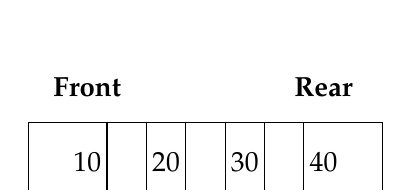
\begin{tikzpicture}[node distance=1cm]
    % Queue cells
    \node (cell1) [draw, rectangle, minimum width=1.5cm, minimum height=1cm] {10};
    \node (cell2) [draw, rectangle, right of=cell1, minimum width=1.5cm, minimum height=1cm] {20};
    \node (cell3) [draw, rectangle, right of=cell2, minimum width=1.5cm, minimum height=1cm] {30};
    \node (cell4) [draw, rectangle, right of=cell3, minimum width=1.5cm, minimum height=1cm] {40};
    
    % Labels for front and rear
    \node[above=0.2cm of cell1] {\textbf{Front}};
    \node[above=0.2cm of cell4] {\textbf{Rear}};
\end{tikzpicture}
\end{center}

\subsection{Priority Queue Diagram}
Below is a diagram for a priority queue. Note that elements are arranged according to priority rather than insertion order.

\begin{center}
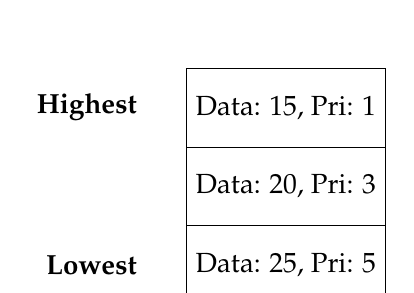
\begin{tikzpicture}[node distance=1cm]
    \node (p1) [draw, rectangle, minimum width=2cm, minimum height=1cm] {Data: 15, Pri: 1};
    \node (p2) [draw, rectangle, below of=p1, minimum width=2cm, minimum height=1cm] {Data: 20, Pri: 3};
    \node (p3) [draw, rectangle, below of=p2, minimum width=2cm, minimum height=1cm] {Data: 25, Pri: 5};
    
    \node[left=0.5cm of p1] {\textbf{Highest}};
    \node[left=0.5cm of p3] {\textbf{Lowest}};
\end{tikzpicture}
\end{center}

\section{C++ Implementations}

\subsection{Queue Using Array}
This implementation uses a fixed-size array. Note that a circular array implementation could handle wrap-around more elegantly, but here we use a simple version.

\begin{lstlisting}[caption={C++ implementation of a Queue using an Array}]
#include <iostream>
using namespace std;
#define MAX 100

class Queue {
private:
    int arr[MAX];
    int front, rear;
public:
    Queue() {
        front = 0;
        rear = -1;
    }
    bool isEmpty() {
        return (front > rear);
    }
    bool isFull() {
        return (rear == MAX - 1);
    }
    void enqueue(int x) {
        if(isFull()) {
            cout << "Queue Overflow\n";
            return;
        }
        arr[++rear] = x;
    }
    int dequeue() {
        if(isEmpty()) {
            cout << "Queue Underflow\n";
            return -1;
        }
        return arr[front++];
    }
    int getFront() {
        if(isEmpty()) {
            cout << "Queue is empty\n";
            return -1;
        }
        return arr[front];
    }
};

int main() {
    Queue q;
    q.enqueue(10);
    q.enqueue(20);
    q.enqueue(30);
    cout << "Front element is: " << q.getFront() << "\n"; // Should print 10
    cout << "Dequeued element is: " << q.dequeue() << "\n"; // Removes 10
    cout << "New front element is: " << q.getFront() << "\n"; // Should print 20
    return 0;
}
\end{lstlisting}

\subsection{Queue Using Linked List}
This implementation uses nodes to allow the queue to grow dynamically.

\begin{lstlisting}[caption={C++ implementation of a Queue using a Linked List}]
#include <iostream>
using namespace std;

class Node {
public:
    int data;
    Node* next;
};

class QueueLL {
private:
    Node* front;
    Node* rear;
public:
    QueueLL() {
        front = rear = nullptr;
    }
    bool isEmpty() {
        return (front == nullptr);
    }
    void enqueue(int x) {
        Node* temp = new Node();
        temp->data = x;
        temp->next = nullptr;
        if(rear == nullptr) {
            front = rear = temp;
            return;
        }
        rear->next = temp;
        rear = temp;
    }
    int dequeue() {
        if(isEmpty()) {
            cout << "Queue Underflow\n";
            return -1;
        }
        int x = front->data;
        Node* temp = front;
        front = front->next;
        if(front == nullptr)
            rear = nullptr;
        delete temp;
        return x;
    }
    int getFront() {
        if(isEmpty()) {
            cout << "Queue is empty\n";
            return -1;
        }
        return front->data;
    }
};

int main() {
    QueueLL q;
    q.enqueue(10);
    q.enqueue(20);
    q.enqueue(30);
    cout << "Front element is: " << q.getFront() << "\n"; // Should print 10
    cout << "Dequeued element is: " << q.dequeue() << "\n"; // Removes 10
    cout << "New front element is: " << q.getFront() << "\n"; // Should print 20
    return 0;
}
\end{lstlisting}

\subsection{Priority Queue Using Array (Unsorted)}
In this version, insertion is \( O(1) \) while deletion (removing the highest priority element) is \( O(n) \).

\begin{lstlisting}[caption={C++ implementation of a Priority Queue using an Array}]
#include <iostream>
using namespace std;
#define MAX 100

struct Element {
    int data;
    int priority;
};

class PriorityQueue {
private:
    Element arr[MAX];
    int size;
public:
    PriorityQueue() {
        size = 0;
    }
    bool isEmpty() {
        return (size == 0);
    }
    bool isFull() {
        return (size == MAX);
    }
    void enqueue(int data, int priority) {
        if(isFull()) {
            cout << "Priority Queue Overflow\n";
            return;
        }
        arr[size].data = data;
        arr[size].priority = priority;
        size++;
    }
    int dequeue() {
        if(isEmpty()) {
            cout << "Priority Queue Underflow\n";
            return -1;
        }
        // Find element with highest priority (lower number indicates higher priority)
        int idx = 0;
        for (int i = 1; i < size; i++) {
            if(arr[i].priority < arr[idx].priority) {
                idx = i;
            }
        }
        int data = arr[idx].data;
        // Remove the element by shifting subsequent elements
        for (int i = idx; i < size - 1; i++) {
            arr[i] = arr[i + 1];
        }
        size--;
        return data;
    }
};

int main() {
    PriorityQueue pq;
    pq.enqueue(100, 3);
    pq.enqueue(200, 1);
    pq.enqueue(300, 2);
    cout << "Dequeued element is: " << pq.dequeue() << "\n"; // Should remove element 200 (highest priority)
    return 0;
}
\end{lstlisting}

\subsection{Priority Queue Using Linked List (Sorted)}
This implementation keeps the list sorted according to priority so that dequeue is \( O(1) \) while insertion takes \( O(n) \).

\begin{lstlisting}[caption={C++ implementation of a Priority Queue using a Linked List}]
#include <iostream>
using namespace std;

class PNode {
public:
    int data;
    int priority;
    PNode* next;
};

class PriorityQueueLL {
private:
    PNode* head;
public:
    PriorityQueueLL() {
        head = nullptr;
    }
    bool isEmpty() {
        return (head == nullptr);
    }
    void enqueue(int data, int priority) {
        PNode* temp = new PNode();
        temp->data = data;
        temp->priority = priority;
        // If list is empty or new node has higher priority than the head
        if(head == nullptr || priority < head->priority) {
            temp->next = head;
            head = temp;
        } else {
            PNode* current = head;
            while(current->next != nullptr && current->next->priority <= priority) {
                current = current->next;
            }
            temp->next = current->next;
            current->next = temp;
        }
    }
    int dequeue() {
        if(isEmpty()) {
            cout << "Priority Queue Underflow\n";
            return -1;
        }
        PNode* temp = head;
        int data = temp->data;
        head = head->next;
        delete temp;
        return data;
    }
    int peek() {
        if(isEmpty()) {
            cout << "Priority Queue is empty\n";
            return -1;
        }
        return head->data;
    }
};

int main() {
    PriorityQueueLL pq;
    pq.enqueue(100, 3);
    pq.enqueue(200, 1);
    pq.enqueue(300, 2);
    cout << "Dequeued element is: " << pq.dequeue() << "\n"; // Should remove element 200 (highest priority)
    return 0;
}
\end{lstlisting}

\section{Example Scenario in Detail}
Consider a standard queue scenario:
\begin{enumerate}
    \item \textbf{Enqueue} 10 \(\rightarrow\) Queue: [10]
    \item \textbf{Enqueue} 20 \(\rightarrow\) Queue: [10, 20]
    \item \textbf{Enqueue} 30 \(\rightarrow\) Queue: [10, 20, 30]
    \item \textbf{Dequeue} \(\rightarrow\) 10 is removed, Queue: [20, 30]
\end{enumerate}

For a priority queue (assuming lower numbers indicate higher priority):
\begin{enumerate}
    \item Enqueue (data: 100, priority: 3)
    \item Enqueue (data: 200, priority: 1)
    \item Enqueue (data: 300, priority: 2)  
\end{enumerate}
After insertion, the elements are ordered by priority as: [200 (priority 1), 300 (priority 2), 100 (priority 3)]. Dequeuing returns 200 first.

\section{Conclusion}
Queues are an essential data structure used in a variety of applications from scheduling to buffering. This chapter presented a detailed theoretical background, discussed time complexities, and illustrated the operations with diagrams. We also provided full C++ implementations for queues and priority queues using both array-based and linked list-based approaches. Understanding these implementations not only helps in grasping the abstract concept of FIFO and priority ordering but also shows practical trade-offs between different implementations.
\chapter{Skip List}

\section{Introduction}
A \textbf{skip list} is a probabilistic data structure that allows fast search, insertion, and deletion operations within an ordered sequence of elements. It achieves performance comparable to balanced trees (average \( O(\log n) \) time for operations) by maintaining multiple levels of linked lists. Higher levels “skip” many nodes, allowing rapid traversal of the list.

\section{Definition and Theoretical Background}
A skip list consists of multiple levels:
\begin{itemize}
    \item The bottom level is an ordinary sorted linked list containing all elements.
    \item Each higher level acts as an “express lane” that skips several elements. Nodes appear in higher levels with a fixed probability \( p \) (commonly \( p=0.5 \)).
\end{itemize}

\subsection{Key Operations}
\begin{itemize}
    \item \textbf{Search}: Start from the topmost level and traverse right until the next node's key exceeds the search key. Then drop down one level and continue. Average search time is \( O(\log n) \).
    \item \textbf{Insertion}: Similar to search, find the correct position at each level and randomly decide how many levels the new node should appear in. Insert the node by updating pointers. Average time is \( O(\log n) \).
    \item \textbf{Deletion}: Search for the node, then update pointers at all levels where the node appears. Average time is \( O(\log n) \).
\end{itemize}

\subsection{Time Complexity}
\begin{itemize}
    \item \textbf{Search}: \( O(\log n) \) average
    \item \textbf{Insertion}: \( O(\log n) \) average
    \item \textbf{Deletion}: \( O(\log n) \) average
\end{itemize}

\section{Diagrams of Skip List Operations}
\subsection{Skip List Structure Diagram}
The diagram below illustrates a skip list with three levels. The bottom level (Level 0) contains all elements. Higher levels (Levels 1 and 2) contain a subset of nodes to enable faster traversal.

\begin{center}
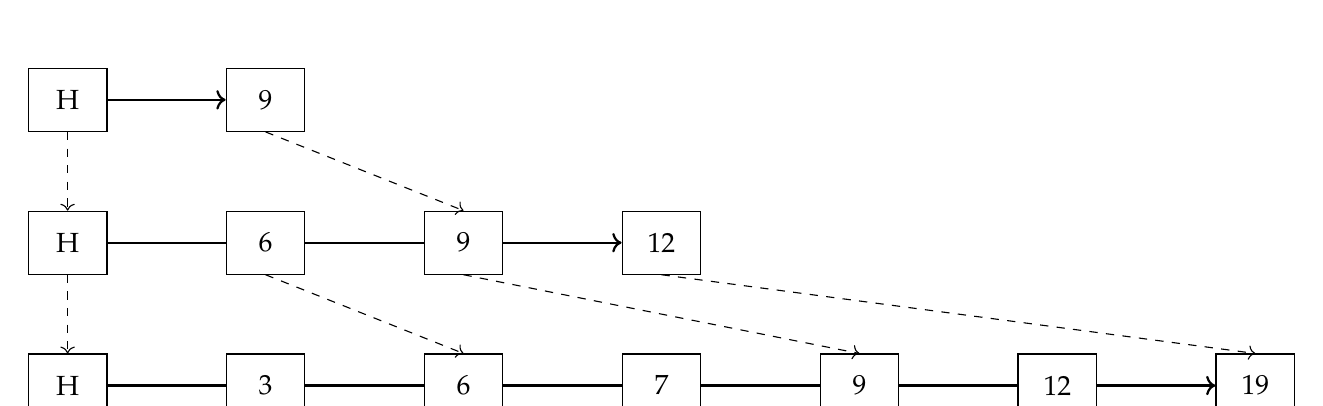
\begin{tikzpicture}[node distance=1cm]
    % Level 2 (top level)
    \node (c0) [draw, rectangle, minimum width=1cm, minimum height=0.8cm] {H};
    \node (c1) [draw, rectangle, right=1.5cm of c0, minimum width=1cm, minimum height=0.8cm] {9};
    \draw[->, thick] (c0) -- (c1);
    
    % Level 1 (middle level)
    \node (b0) [draw, rectangle, minimum width=1cm, minimum height=0.8cm, below=of c0] {H};
    \node (b1) [draw, rectangle, right=1.5cm of b0, minimum width=1cm, minimum height=0.8cm] {6};
    \node (b2) [draw, rectangle, right=1.5cm of b1, minimum width=1cm, minimum height=0.8cm] {9};
    \node (b3) [draw, rectangle, right=1.5cm of b2, minimum width=1cm, minimum height=0.8cm] {12};
    \draw[->, thick] (b0) -- (b1) -- (b2) -- (b3);
    
    % Level 0 (bottom level)
    \node (a0) [draw, rectangle, minimum width=1cm, minimum height=0.8cm, below=of b0] {H};
    \node (a1) [draw, rectangle, right=1.5cm of a0, minimum width=1cm, minimum height=0.8cm] {3};
    \node (a2) [draw, rectangle, right=1.5cm of a1, minimum width=1cm, minimum height=0.8cm] {6};
    \node (a3) [draw, rectangle, right=1.5cm of a2, minimum width=1cm, minimum height=0.8cm] {7};
    \node (a4) [draw, rectangle, right=1.5cm of a3, minimum width=1cm, minimum height=0.8cm] {9};
    \node (a5) [draw, rectangle, right=1.5cm of a4, minimum width=1cm, minimum height=0.8cm] {12};
    \node (a6) [draw, rectangle, right=1.5cm of a5, minimum width=1cm, minimum height=0.8cm] {19};
    \draw[->, thick] (a0) -- (a1) -- (a2) -- (a3) -- (a4) -- (a5) -- (a6);
    
    % Vertical links from Level 2 to Level 1
    \draw[->, dashed] (c0.south) -- (b0.north);
    \draw[->, dashed] (c1.south) -- (b2.north);
    
    % Vertical links from Level 1 to Level 0
    \draw[->, dashed] (b0.south) -- (a0.north);
    \draw[->, dashed] (b1.south) -- (a2.north);
    \draw[->, dashed] (b2.south) -- (a4.north);
    \draw[->, dashed] (b3.south) -- (a6.north);
\end{tikzpicture}
\end{center}

In the diagram:
\begin{itemize}
    \item \textbf{H} stands for the header node.
    \item Dashed arrows indicate pointers connecting nodes between levels.
\end{itemize}

\section{C++ Implementation of a Skip List}
Below is a sample C++ implementation of a skip list that supports search, insertion, and deletion operations.

\begin{lstlisting}[caption={C++ implementation of a Skip List}]
#include <iostream>
#include <cstdlib>
#include <climits>
#include <ctime>
using namespace std;

class Node {
public:
    int key;
    Node **forward;
    // Constructor: creates a node with given key and level
    Node(int key, int level) : key(key) {
        forward = new Node*[level + 1];
        for (int i = 0; i <= level; i++) {
            forward[i] = nullptr;
        }
    }
    ~Node() {
        delete [] forward;
    }
};

class SkipList {
    int maxLevel;
    float p;
    int level;
    Node *header;
public:
    SkipList(int maxLevel, float p) : maxLevel(maxLevel), p(p), level(0) {
        // Create header node with key -1 (a sentinel) and maximum level
        header = new Node(-1, maxLevel);
    }
    ~SkipList() {
        // Free nodes (not fully implemented for brevity)
        delete header;
    }
    
    // Randomly generate a level for node
    int randomLevel() {
        int lvl = 0;
        while (((float)rand() / RAND_MAX) < p && lvl < maxLevel)
            lvl++;
        return lvl;
    }
    
    // Insert a key into skip list
    void insertElement(int key) {
        Node *current = header;
        Node *update[maxLevel + 1];
        for (int i = 0; i <= maxLevel; i++) {
            update[i] = nullptr;
        }
        // Start from highest level and move downwards
        for (int i = level; i >= 0; i--) {
            while (current->forward[i] != nullptr && current->forward[i]->key < key)
                current = current->forward[i];
            update[i] = current;
        }
        current = current->forward[0];
        // If key not found, insert new node
        if (current == nullptr || current->key != key) {
            int rlevel = randomLevel();
            if (rlevel > level) {
                for (int i = level + 1; i <= rlevel; i++) {
                    update[i] = header;
                }
                level = rlevel;
            }
            Node* n = new Node(key, rlevel);
            for (int i = 0; i <= rlevel; i++) {
                n->forward[i] = update[i]->forward[i];
                update[i]->forward[i] = n;
            }
            cout << "Successfully inserted key " << key << "\n";
        }
    }
    
    // Delete an element from skip list
    void deleteElement(int key) {
        Node *current = header;
        Node *update[maxLevel + 1];
        for (int i = 0; i <= maxLevel; i++) {
            update[i] = nullptr;
        }
        for (int i = level; i >= 0; i--) {
            while (current->forward[i] != nullptr && current->forward[i]->key < key)
                current = current->forward[i];
            update[i] = current;
        }
        current = current->forward[0];
        if (current != nullptr && current->key == key) {
            for (int i = 0; i <= level; i++) {
                if (update[i]->forward[i] != current)
                    break;
                update[i]->forward[i] = current->forward[i];
            }
            delete current;
            while (level > 0 && header->forward[level] == nullptr)
                level--;
            cout << "Successfully deleted key " << key << "\n";
        }
    }
    
    // Search for an element in the skip list
    Node* searchElement(int key) {
        Node *current = header;
        for (int i = level; i >= 0; i--) {
            while (current->forward[i] != nullptr && current->forward[i]->key < key)
                current = current->forward[i];
        }
        current = current->forward[0];
        if (current != nullptr && current->key == key)
            return current;
        return nullptr;
    }
    
    // Display the skip list levels
    void displayList() {
        cout << "\n***** Skip List *****" << "\n";
        for (int i = 0; i <= level; i++) {
            Node *node = header->forward[i];
            cout << "Level " << i << ": ";
            while (node != nullptr) {
                cout << node->key << " ";
                node = node->forward[i];
            }
            cout << "\n";
        }
    }
};

int main() {
    srand((unsigned)time(0));
    SkipList lst(3, 0.5);
    lst.insertElement(3);
    lst.insertElement(6);
    lst.insertElement(7);
    lst.insertElement(9);
    lst.insertElement(12);
    lst.insertElement(19);
    lst.displayList();
    
    int searchKey = 9;
    Node *res = lst.searchElement(searchKey);
    if(res != nullptr)
        cout << "Found key: " << searchKey << "\n";
    else
        cout << "Key " << searchKey << " not found\n";
    
    lst.deleteElement(3);
    lst.displayList();
    
    return 0;
}
\end{lstlisting}

\section{Example Scenario in Detail}
Consider the following operations on an initially empty skip list:
\begin{enumerate}
    \item \textbf{Insert} 3, 6, 7, 9, 12, 19 into the skip list.
    \item The skip list will organize these keys into multiple levels where higher levels contain fewer nodes.
    \item \textbf{Search} for key 9: Starting from the top level, the algorithm quickly narrows down to the correct node.
    \item \textbf{Delete} key 3: After deletion, pointers at all levels are updated accordingly.
\end{enumerate}

\section{Conclusion}
Skip lists offer an elegant probabilistic alternative to balanced trees, providing \( O(\log n) \) average time for search, insertion, and deletion. This chapter presented the theoretical background, detailed operations, and diagrams illustrating the multi-level structure. The included C++ implementation demonstrates how a skip list can be built and manipulated, making it a powerful tool for ordered data storage and retrieval.

\part{Non-linear Data Structures}
\chapter{Tree Data Structures}

\section{Introduction}
A \textbf{tree} is a hierarchical data structure that consists of nodes connected by edges. Trees are widely used in computer science to represent hierarchical relationships such as file systems, organizational structures, and decision processes. A \textbf{binary tree} is a tree in which each node has at most two children, commonly referred to as the left and right child. A \textbf{binary search tree (BST)} is a special kind of binary tree that maintains an order: for any node, all elements in its left subtree are less than or equal to the node's key and all elements in its right subtree are greater.

\section{Definition, Terminology, and Formulas}
\subsection{Basic Definitions and Terminology}
A tree \( T \) is defined as a pair \( (V, E) \) where:
\begin{itemize}
    \item \( V \) is a set of nodes.
    \item \( E \) is a set of edges connecting the nodes.
\end{itemize}
Key terms include:
\begin{description}
    \item[Root:] The topmost node in a tree.
    \item[Parent:] A node that has one or more children.
    \item[Child:] A node that is a descendant of another node.
    \item[Leaf:] A node with no children.
    \item[Subtree:] A tree consisting of a node and its descendants.
    \item[Height:] The length of the longest path from the root to a leaf. Formally, for a node \( v \), 
    \[
    \text{height}(v) = \begin{cases} 
    0, & \text{if } v \text{ is a leaf,} \\
    1 + \max(\text{height}(v.\text{left}), \text{height}(v.\text{right})), & \text{otherwise.}
    \end{cases}
    \]
    \item[Depth:] The length of the path from the root to the node.
\end{description}

\subsection{Performance Formulas}
For a balanced binary tree containing \( n \) nodes:
\begin{itemize}
    \item \textbf{Search, Insertion, Deletion:} Average time complexity is \( O(\log n) \).
\end{itemize}
In a degenerate (unbalanced) tree, these operations degrade to \( O(n) \).

\subsection{Summary Table of Tree Properties}
\begin{table}[h!]
\centering
\small
\begin{tabular}{p{3.5cm} p{3cm} p{4cm} p{3cm}}
\toprule
\textbf{Tree Type} & \textbf{Average Height} & \textbf{Search / Insertion / Deletion} & \textbf{Space Complexity} \\
\midrule
Binary Search Tree (Balanced)   & \( O(\log n) \) & \( O(\log n) \) & \( O(n) \) \\
Binary Search Tree (Unbalanced) & \( O(n) \)      & \( O(n) \)      & \( O(n) \) \\
AVL Tree / Red-Black Tree       & \( O(\log n) \) & \( O(\log n) \) & \( O(n) \) \\
Complete Binary Tree            & \( O(\log n) \) & \( O(\log n) \) & \( O(n) \) \\
\bottomrule
\end{tabular}
\caption{Comparison of Tree Data Structures}
\label{tab:tree-comparison}
\normalsize
\end{table}





\section{Types of Tree Data Structures}
Trees come in many forms, each with its own characteristics:
\begin{itemize}
    \item \textbf{Binary Tree}: Each node has at most two children.
    \item \textbf{Binary Search Tree (BST)}: A binary tree that maintains sorted order.
    \item \textbf{Balanced Trees}: Such as AVL trees and Red-Black trees, which maintain \( O(\log n) \) height.
    \item \textbf{Complete Binary Tree}: A binary tree in which all levels, except possibly the last, are completely filled.
    \item \textbf{Heap}: A specialized tree-based structure that satisfies the heap property (used for priority queues).
    \item \textbf{B-tree and B+ tree}: Used in databases and filesystems, designed to work well on disks.
    \item \textbf{Trie}: A tree used for storing associative arrays where the keys are usually strings.
\end{itemize}

\section{Converting Arrays into Trees}
A common example is converting an array into a \textbf{complete binary tree}. If we have an array \( A \) with \( n \) elements, we can represent it as a complete binary tree where:
\begin{itemize}
    \item The element at index \( i \) is the parent.
    \item The left child is at index \( 2i+1 \).
    \item The right child is at index \( 2i+2 \).
\end{itemize}
This representation is particularly efficient because it uses the array indices to simulate pointers, which is common in heap implementations.

\section{Diagrams of Tree Structures and Traversals}
\subsection{Binary Tree Diagram}
The diagram below shows a simple binary tree:

\begin{center}
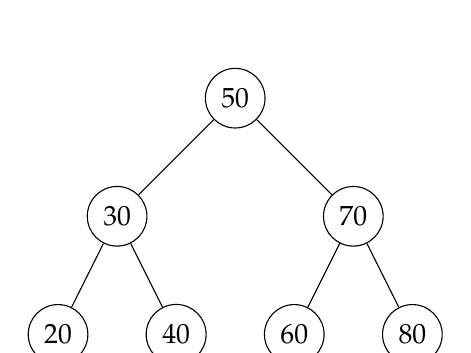
\begin{tikzpicture}[level distance=1.5cm,
  level 1/.style={sibling distance=3cm},
  level 2/.style={sibling distance=1.5cm}]
  \node [draw, circle] {50}
    child { node [draw, circle] {30}
      child { node [draw, circle] {20} }
      child { node [draw, circle] {40} }
    }
    child { node [draw, circle] {70}
      child { node [draw, circle] {60} }
      child { node [draw, circle] {80} }
    };
\end{tikzpicture}
\end{center}

\subsection{Traversal Order Example}
For the tree above:
\begin{itemize}
    \item \textbf{Preorder}: 50, 30, 20, 40, 70, 60, 80
    \item \textbf{Inorder}: 20, 30, 40, 50, 60, 70, 80
    \item \textbf{Postorder}: 20, 40, 30, 60, 80, 70, 50
    \item \textbf{Level Order}: 50, 30, 70, 20, 40, 60, 80
\end{itemize}

\section{C++ Implementation of a Binary Search Tree}
Below is a complete C++ implementation of a binary search tree (BST) including insertion, search, deletion, and all traversal methods.

\begin{lstlisting}[caption={C++ implementation of a Binary Search Tree}]
#include <iostream>
#include <queue>
using namespace std;

struct Node {
    int key;
    Node* left;
    Node* right;
    Node(int key) : key(key), left(nullptr), right(nullptr) {}
};

class BST {
private:
    Node* root;
    
    Node* insert(Node* node, int key) {
        if (node == nullptr)
            return new Node(key);
        if (key < node->key)
            node->left = insert(node->left, key);
        else if (key > node->key)
            node->right = insert(node->right, key);
        return node;
    }
    
    Node* search(Node* node, int key) {
        if (node == nullptr || node->key == key)
            return node;
        if (key < node->key)
            return search(node->left, key);
        else
            return search(node->right, key);
    }
    
    // Find the minimum node in a subtree
    Node* minValueNode(Node* node) {
        Node* current = node;
        while (current && current->left != nullptr)
            current = current->left;
        return current;
    }
    
    Node* remove(Node* node, int key) {
        if (node == nullptr) return node;
        if (key < node->key)
            node->left = remove(node->left, key);
        else if (key > node->key)
            node->right = remove(node->right, key);
        else {
            // Node with only one child or no child
            if (node->left == nullptr) {
                Node* temp = node->right;
                delete node;
                return temp;
            } else if (node->right == nullptr) {
                Node* temp = node->left;
                delete node;
                return temp;
            }
            // Node with two children: Get the inorder successor (smallest in the right subtree)
            Node* temp = minValueNode(node->right);
            node->key = temp->key;
            node->right = remove(node->right, temp->key);
        }
        return node;
    }
    
    // Preorder Traversal (Root, Left, Right)
    void preorder(Node* node) {
        if (node != nullptr) {
            cout << node->key << " ";
            preorder(node->left);
            preorder(node->right);
        }
    }
    
    // Inorder Traversal (Left, Root, Right)
    void inorder(Node* node) {
        if (node != nullptr) {
            inorder(node->left);
            cout << node->key << " ";
            inorder(node->right);
        }
    }
    
    // Postorder Traversal (Left, Right, Root)
    void postorder(Node* node) {
        if (node != nullptr) {
            postorder(node->left);
            postorder(node->right);
            cout << node->key << " ";
        }
    }
    
public:
    BST() : root(nullptr) {}
    
    void insert(int key) {
        root = insert(root, key);
    }
    
    Node* search(int key) {
        return search(root, key);
    }
    
    void remove(int key) {
        root = remove(root, key);
    }
    
    void preorder() {
        preorder(root);
        cout << "\n";
    }
    
    void inorder() {
        inorder(root);
        cout << "\n";
    }
    
    void postorder() {
        postorder(root);
        cout << "\n";
    }
    
    // Level Order Traversal (Breadth-first)
    void levelOrder() {
        if (root == nullptr) return;
        queue<Node*> q;
        q.push(root);
        while (!q.empty()) {
            Node* current = q.front();
            q.pop();
            cout << current->key << " ";
            if (current->left != nullptr)
                q.push(current->left);
            if (current->right != nullptr)
                q.push(current->right);
        }
        cout << "\n";
    }
};

int main() {
    BST tree;
    // Insertion
    tree.insert(50);
    tree.insert(30);
    tree.insert(20);
    tree.insert(40);
    tree.insert(70);
    tree.insert(60);
    tree.insert(80);
    
    cout << "Inorder Traversal: ";
    tree.inorder();      // 20 30 40 50 60 70 80
    
    cout << "Preorder Traversal: ";
    tree.preorder();     // 50 30 20 40 70 60 80
    
    cout << "Postorder Traversal: ";
    tree.postorder();    // 20 40 30 60 80 70 50
    
    cout << "Level Order Traversal: ";
    tree.levelOrder();   // 50 30 70 20 40 60 80
    
    // Search for a key
    int searchKey = 40;
    if (tree.search(searchKey))
        cout << "Key " << searchKey << " found in the tree.\n";
    else
        cout << "Key " << searchKey << " not found in the tree.\n";
    
    // Deletion
    tree.remove(30);
    cout << "Inorder Traversal after deleting 30: ";
    tree.inorder();
    
    return 0;
}
\end{lstlisting}

\section{AVL Trees: Implementation and Rotations}
AVL trees are a type of self-balancing binary search tree that ensures the difference in heights (balance factor) between the left and right subtrees for any node is at most one. This guarantees \( O(\log n) \) time complexity for search, insertion, and deletion.

\subsection{Node Structure and Balance Factor}
For an AVL tree, each node is augmented with a \textbf{height} attribute. The \textbf{balance factor} is defined as:
\[
\text{Balance Factor} = \text{height(left subtree)} - \text{height(right subtree)}
\]
A node is balanced if its balance factor is \(-1\), \(0\), or \(1\).

\subsection{AVL Rotations}
To restore balance after an insertion or deletion, AVL trees perform rotations:
\begin{itemize}
    \item \textbf{Right Rotation}: Used for a left-left imbalance.
    \item \textbf{Left Rotation}: Used for a right-right imbalance.
    \item \textbf{Left-Right Rotation}: A left rotation followed by a right rotation, used for a left-right imbalance.
    \item \textbf{Right-Left Rotation}: A right rotation followed by a left rotation, used for a right-left imbalance.
\end{itemize}

\subsection{Diagram: Left Rotation Example}
Before rotation (inserting keys causing a right-right imbalance):
\begin{center}
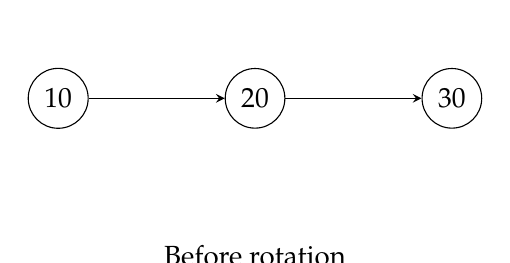
\begin{tikzpicture}[>=stealth, node distance=1.5cm]
    \node[draw, circle] (x) {10};
    \node[draw, circle, right of=x, xshift=1cm] (y) {20};
    \node[draw, circle, right of=y, xshift=1cm] (z) {30};
    \draw[->] (x) -- (y);
    \draw[->] (y) -- (z);
    \node[below of=y, yshift=-0.5cm] {Before rotation};
\end{tikzpicture}
\end{center}

After performing a left rotation at node 10, the tree becomes:
\begin{center}
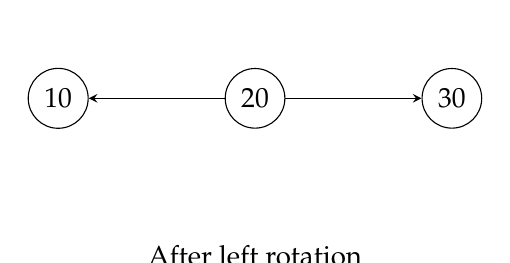
\begin{tikzpicture}[>=stealth, node distance=1.5cm]
    \node[draw, circle] (y) {20};
    \node[draw, circle, left of=y, xshift=-1cm] (x) {10};
    \node[draw, circle, right of=y, xshift=1cm] (z) {30};
    \draw[->] (y) -- (x);
    \draw[->] (y) -- (z);
    \node[below of=y, yshift=-0.5cm] {After left rotation};
\end{tikzpicture}
\end{center}

\subsection{C++ Implementation of an AVL Tree}
Below is a complete C++ implementation for an AVL tree that includes node structure, insertion with rebalancing (rotations), and a preorder traversal function for demonstration.

\begin{lstlisting}[caption={C++ implementation of an AVL Tree}]
#include <iostream>
#include <algorithm>
using namespace std;

struct AVLNode {
    int key;
    int height;
    AVLNode *left, *right;
    AVLNode(int key) : key(key), height(1), left(nullptr), right(nullptr) {}
};

int height(AVLNode *node) {
    return node ? node->height : 0;
}

int getBalance(AVLNode *node) {
    return node ? height(node->left) - height(node->right) : 0;
}

AVLNode* rightRotate(AVLNode* y) {
    AVLNode *x = y->left;
    AVLNode *T2 = x->right;
    // Perform rotation
    x->right = y;
    y->left = T2;
    // Update heights
    y->height = max(height(y->left), height(y->right)) + 1;
    x->height = max(height(x->left), height(x->right)) + 1;
    return x;
}

AVLNode* leftRotate(AVLNode* x) {
    AVLNode *y = x->right;
    AVLNode *T2 = y->left;
    // Perform rotation
    y->left = x;
    x->right = T2;
    // Update heights
    x->height = max(height(x->left), height(x->right)) + 1;
    y->height = max(height(y->left), height(y->right)) + 1;
    return y;
}

AVLNode* insert(AVLNode* node, int key) {
    // Standard BST insertion
    if(!node)
       return new AVLNode(key);
    if(key < node->key)
       node->left = insert(node->left, key);
    else if(key > node->key)
       node->right = insert(node->right, key);
    else
       return node; // no duplicates allowed

    // Update the height of this ancestor node
    node->height = max(height(node->left), height(node->right)) + 1;
    int balance = getBalance(node);

    // Left Left Case
    if(balance > 1 && key < node->left->key)
        return rightRotate(node);
    // Right Right Case
    if(balance < -1 && key > node->right->key)
        return leftRotate(node);
    // Left Right Case
    if(balance > 1 && key > node->left->key) {
        node->left = leftRotate(node->left);
        return rightRotate(node);
    }
    // Right Left Case
    if(balance < -1 && key < node->right->key) {
        node->right = rightRotate(node->right);
        return leftRotate(node);
    }
    return node;
}

void preOrder(AVLNode *root) {
    if(root != nullptr) {
        cout << root->key << " ";
        preOrder(root->left);
        preOrder(root->right);
    }
}

int main() {
    AVLNode *root = nullptr;
    int arr[] = {10, 20, 30, 40, 50, 25};
    for (int i = 0; i < 6; i++)
        root = insert(root, arr[i]);
    cout << "Preorder traversal of the constructed AVL tree is: \n";
    preOrder(root);
    return 0;
}
\end{lstlisting}

\section{AVL Trees: Rotations}

AVL trees are a type of self-balancing binary search tree that ensures the difference in heights (balance factor) between the left and right subtrees for any node is at most one. This guarantees \( O(\log n) \) time complexity for search, insertion, and deletion.

\subsection{Node Structure and Balance Factor}
For an AVL tree, each node is augmented with a \textbf{height} attribute. The \textbf{balance factor} of a node is defined as:
\[
\text{Balance Factor} = \text{height(left subtree)} - \text{height(right subtree)}
\]
A node is balanced if its balance factor is \(-1\), \(0\), or \(1\).

\subsection{AVL Rotations: Terminology and Diagrams}
When an insertion or deletion causes a node's balance factor to fall outside of \([-1, 1]\), the AVL tree must be rebalanced using rotations. The key rotation types are:

\begin{itemize}
    \item \textbf{Right Rotation}: Corrects a left-left imbalance.
    \item \textbf{Left Rotation}: Corrects a right-right imbalance.
    \item \textbf{Left-Right Rotation}: A combination; perform a left rotation on the left child, then a right rotation on the node.
    \item \textbf{Right-Left Rotation}: A combination; perform a right rotation on the right child, then a left rotation on the node.
\end{itemize}

\subsubsection{Right Rotation Diagram}
\textbf{Right Rotation} is used when a node's left subtree is heavy (i.e., a left-left imbalance). Consider the following subtree:

\textbf{Before right rotation:}
\begin{center}
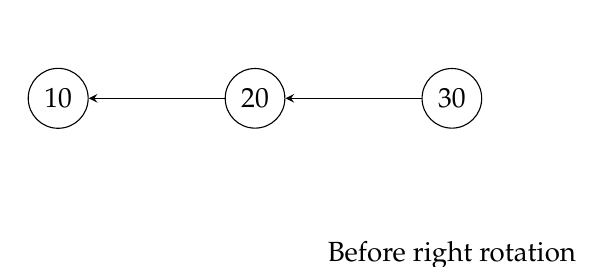
\begin{tikzpicture}[>=stealth, node distance=1.5cm]
    \node[draw, circle] (y) {30};
    \node[draw, circle, left of=y, xshift=-1cm] (x) {20};
    \node[draw, circle, left of=x, xshift=-1cm] (T1) {10};
    \draw[->] (x) -- (T1);
    \draw[->] (y) -- (x);
    \node[below of=y, yshift=-0.5cm] {Before right rotation};
\end{tikzpicture}
\end{center}

\textbf{After right rotation at node \(y\):}
\begin{center}
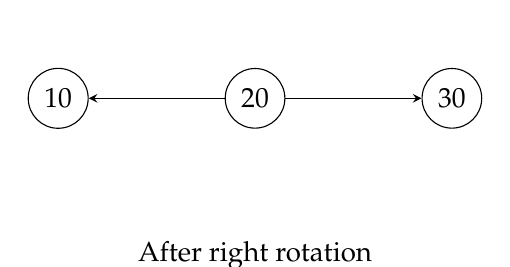
\begin{tikzpicture}[>=stealth, node distance=1.5cm]
    \node[draw, circle] (x) {20};
    \node[draw, circle, right of=x, xshift=1cm] (y) {30};
    \node[draw, circle, left of=x, xshift=-1cm] (T1) {10};
    \draw[->] (x) -- (T1);
    \draw[->] (x) -- (y);
    \node[below of=x, yshift=-0.5cm] {After right rotation};
\end{tikzpicture}
\end{center}

\subsubsection{Left Rotation Diagram}
\textbf{Left Rotation} is used when a node's right subtree is heavy (i.e., a right-right imbalance). Consider the following subtree:

\textbf{Before left rotation:}
\begin{center}
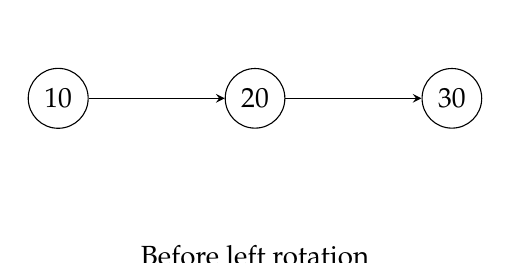
\begin{tikzpicture}[>=stealth, node distance=1.5cm]
    \node[draw, circle] (x) {10};
    \node[draw, circle, right of=x, xshift=1cm] (y) {20};
    \node[draw, circle, right of=y, xshift=1cm] (z) {30};
    \draw[->] (x) -- (y);
    \draw[->] (y) -- (z);
    \node[below of=y, yshift=-0.5cm] {Before left rotation};
\end{tikzpicture}
\end{center}

\textbf{After left rotation at node \(x\):}
\begin{center}
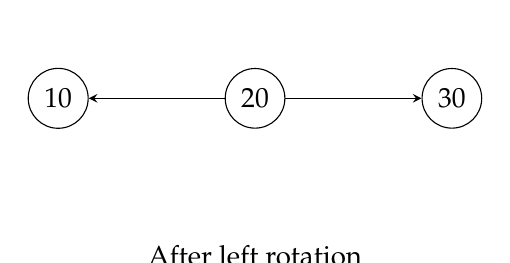
\begin{tikzpicture}[>=stealth, node distance=1.5cm]
    \node[draw, circle] (y) {20};
    \node[draw, circle, left of=y, xshift=-1cm] (x) {10};
    \node[draw, circle, right of=y, xshift=1cm] (z) {30};
    \draw[->] (y) -- (x);
    \draw[->] (y) -- (z);
    \node[below of=y, yshift=-0.5cm] {After left rotation};
\end{tikzpicture}
\end{center}

\section{Conclusion}
This chapter has provided an in-depth exploration of tree data structures. We began with the theoretical foundations and key terminology, introduced essential formulas, and presented a summary table of tree properties. We then discussed various types of trees—including binary trees, binary search trees, balanced trees, heaps, and tries—and explained how to convert an array into a complete binary tree.
\chapter{Graph Data Structures}

\section{Introduction}
A \textbf{graph} is a data structure used to represent a set of objects (called \textbf{vertices} or \textbf{nodes}) and the relationships between them (called \textbf{edges}). Graphs are widely used to model many real-world problems such as social networks, transportation systems, and web page link structures. Depending on the application, graphs can be:
\begin{itemize}
    \item \textbf{Directed} (where edges have a direction).
    \item \textbf{Undirected} (where edges are bidirectional).
    \item \textbf{Weighted} (if edges carry a cost, distance, or other metric).
\end{itemize}

\section{Definition, Terminology, and Formulas}
A graph \( G \) is defined as a pair \( (V, E) \), where:
\begin{itemize}
    \item \( V \) is a non-empty set of vertices.
    \item \( E \) is a set of edges, where each edge is a pair (or ordered pair in directed graphs) of vertices.
\end{itemize}

\subsection{Key Terminology}
\begin{description}
    \item[Vertex (Node):] An individual object in the graph.
    \item[Edge: ] A connection between two vertices.
    \item[Adjacent: ] Two vertices that are directly connected by an edge.
    \item[Degree: ] For an undirected graph, the degree of a vertex is the number of edges incident on it. In directed graphs, we differentiate between \textbf{in-degree} and \textbf{out-degree}.
    \item[Path: ] A sequence of vertices connected by edges.
    \item[Cycle: ] A path that starts and ends at the same vertex without repeating an edge.
    \item[Connectivity: ] A graph is connected if there is a path between any two vertices.
\end{description}

\subsection{Useful Formulas}
\begin{itemize}
    \item \textbf{Handshaking Lemma (Undirected):} 
    \[
    \sum_{v \in V} \text{degree}(v) = 2|E|
    \]
    \item \textbf{Directed Graph Degree Relationship:}
    \[
    \sum_{v \in V} \text{in-degree}(v) = \sum_{v \in V} \text{out-degree}(v) = |E|
    \]
    \item \textbf{Path Length:} The length of a path is defined as the number of edges in the path.
\end{itemize}

\section{Graph Representations}
Graphs can be represented in several ways. The two primary methods are:

\subsection{Adjacency Matrix}
An adjacency matrix is a 2D array \( A \) of size \( |V| \times |V| \) where:
\[
A[i][j] = \begin{cases}
1 & \text{if there is an edge from vertex } i \text{ to vertex } j, \\
0 & \text{otherwise.}
\end{cases}
\]
For weighted graphs, the entry may store the edge weight instead of 1 (with a special value such as \(\infty\) or 0 indicating no edge).

\subsection{Adjacency List}
An adjacency list represents the graph as an array (or vector) of lists. The list at index \( i \) contains all vertices adjacent to vertex \( i \). This representation is especially space-efficient for sparse graphs.

\subsection{Edge List}
An edge list is simply a list of all edges. Each edge is represented by a pair (or triple for weighted graphs) of vertices:
\[
\text{Edge List } = \{(u,v) \mid u, v \in V\}
\]
This representation is simple and is often used as an intermediate step in algorithms like Kruskal's for finding minimum spanning trees.

\section{Types of Graphs and Detailed Diagrams}
Graphs can be categorized based on the nature of their edges and vertices:

\subsection{Undirected Graph}
In an undirected graph, the edges do not have a direction. An edge between vertices \( u \) and \( v \) is represented as \( \{u, v\} \).

\textbf{Diagram:}
\begin{center}
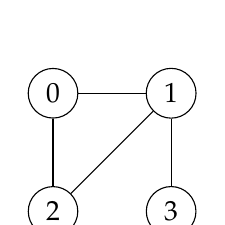
\begin{tikzpicture}[node distance=1.5cm, auto]
    \node[draw, circle] (v0) {0};
    \node[draw, circle, right of=v0] (v1) {1};
    \node[draw, circle, below of=v0] (v2) {2};
    \node[draw, circle, right of=v2] (v3) {3};
    \draw (v0) -- (v1);
    \draw (v0) -- (v2);
    \draw (v1) -- (v2);
    \draw (v1) -- (v3);
\end{tikzpicture}
\end{center}

\subsection{Directed Graph (Digraph)}
In a directed graph, each edge has a direction. An edge from vertex \( u \) to vertex \( v \) is represented as \( (u, v) \).

\textbf{Diagram:}
\begin{center}
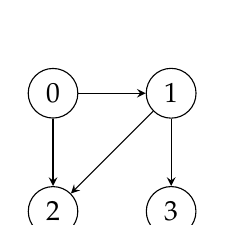
\begin{tikzpicture}[node distance=1.5cm, auto, ->,>=stealth]
    \node[draw, circle] (v0) {0};
    \node[draw, circle, right of=v0] (v1) {1};
    \node[draw, circle, below of=v0] (v2) {2};
    \node[draw, circle, right of=v2] (v3) {3};
    \draw (v0) edge (v1);
    \draw (v0) edge (v2);
    \draw (v1) edge (v2);
    \draw (v1) edge (v3);
\end{tikzpicture}
\end{center}

\subsection{Weighted Graph}
A weighted graph has weights (or costs) associated with each edge. These weights can represent distances, costs, or other metrics.

\textbf{Diagram (Undirected Weighted Graph):}
\begin{center}
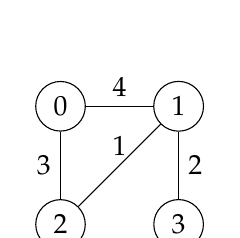
\begin{tikzpicture}[node distance=1.5cm, auto]
    \node[draw, circle] (v0) {0};
    \node[draw, circle, right of=v0] (v1) {1};
    \node[draw, circle, below of=v0] (v2) {2};
    \node[draw, circle, right of=v2] (v3) {3};
    \draw (v0) -- node[midway, above] {4} (v1);
    \draw (v0) -- node[midway, left] {3} (v2);
    \draw (v1) -- node[midway, right] {2} (v3);
    \draw (v1) -- node[midway, above] {1} (v2);
\end{tikzpicture}
\end{center}

\section{C++ Implementations of Graph Representations}
Below are sample C++ implementations for the different graph representations.

\subsection{Adjacency Matrix Implementation}
\begin{lstlisting}[caption={C++ implementation using an Adjacency Matrix}]
#include <iostream>
#include <vector>
using namespace std;

class GraphMatrix {
private:
    int V; // number of vertices
    vector<vector<int>> adjMatrix;
public:
    GraphMatrix(int V) : V(V) {
        adjMatrix.resize(V, vector<int>(V, 0));
    }
    void addEdge(int u, int v, bool undirected = true, int weight = 1) {
        adjMatrix[u][v] = weight;
        if(undirected)
            adjMatrix[v][u] = weight;
    }
    void printMatrix() {
        for(int i = 0; i < V; i++) {
            for(int j = 0; j < V; j++)
                cout << adjMatrix[i][j] << " ";
            cout << "\n";
        }
    }
};

int main() {
    int V = 4;
    GraphMatrix graph(V);
    graph.addEdge(0, 1);
    graph.addEdge(0, 2);
    graph.addEdge(1, 2);
    graph.addEdge(1, 3);
    cout << "Adjacency Matrix:\n";
    graph.printMatrix();
    return 0;
}
\end{lstlisting}

\subsection{Adjacency List Implementation}
\begin{lstlisting}[caption={C++ implementation using an Adjacency List}]
#include <iostream>
#include <vector>
using namespace std;

class GraphList {
private:
    int V;
    vector<vector<int>> adjList;
public:
    GraphList(int V) : V(V) {
        adjList.resize(V);
    }
    void addEdge(int u, int v, bool undirected = true) {
        adjList[u].push_back(v);
        if(undirected)
            adjList[v].push_back(u);
    }
    void printList() {
        for(int i = 0; i < V; i++) {
            cout << "Vertex " << i << ": ";
            for(auto v : adjList[i])
                cout << v << " ";
            cout << "\n";
        }
    }
};

int main() {
    int V = 4;
    GraphList graph(V);
    graph.addEdge(0, 1);
    graph.addEdge(0, 2);
    graph.addEdge(1, 2);
    graph.addEdge(1, 3);
    cout << "Adjacency List:\n";
    graph.printList();
    return 0;
}
\end{lstlisting}

\subsection{Edge List Representation}
\begin{lstlisting}[caption={C++ implementation using an Edge List}]
#include <iostream>
#include <vector>
using namespace std;

class GraphEdgeList {
private:
    int V;
    vector<pair<int, int>> edgeList;
public:
    GraphEdgeList(int V) : V(V) { }
    void addEdge(int u, int v) {
        edgeList.push_back({u, v});
    }
    void printEdges() {
        for(auto edge : edgeList)
            cout << edge.first << " - " << edge.second << "\n";
    }
};

int main() {
    int V = 4;
    GraphEdgeList graph(V);
    graph.addEdge(0, 1);
    graph.addEdge(0, 2);
    graph.addEdge(1, 2);
    graph.addEdge(1, 3);
    cout << "Edge List:\n";
    graph.printEdges();
    return 0;
}
\end{lstlisting}

\section{Graph Algorithms}

In this section we discuss two fundamental graph traversal algorithms: Breadth-First Search (BFS) and Depth-First Search (DFS). We also include a discussion on spanning trees, which are subgraphs connecting all vertices without cycles.

\subsection{Breadth-First Search (BFS)}
BFS is a level-order traversal that visits nodes layer by layer. It uses a queue to keep track of the next vertex to visit.

\textbf{BFS Diagram:}
\begin{center}
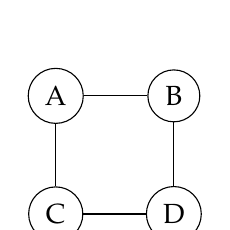
\begin{tikzpicture}[node distance=1.5cm, auto]
    \node[draw, circle] (A) {A};
    \node[draw, circle, right of=A] (B) {B};
    \node[draw, circle, below of=A] (C) {C};
    \node[draw, circle, right of=C] (D) {D};
    \draw (A) -- (B);
    \draw (A) -- (C);
    \draw (B) -- (D);
    \draw (C) -- (D);
\end{tikzpicture}
\end{center}

\textbf{BFS Pseudocode:}
\begin{lstlisting}
BFS(Graph, start):
    create a queue Q
    mark start as visited and enqueue start
    while Q is not empty:
        v = Q.dequeue()
        for all neighbors w of v:
            if w is not visited:
                mark w as visited
                enqueue w
\end{lstlisting}

\subsubsection{BFS C++ Implementation}
\begin{lstlisting}[caption={BFS in C++ using an Adjacency List}]
#include <iostream>
#include <vector>
#include <queue>
using namespace std;

void BFS(const vector<vector<int>>& adjList, int start) {
    int V = adjList.size();
    vector<bool> visited(V, false);
    queue<int> q;

    visited[start] = true;
    q.push(start);

    while (!q.empty()) {
        int v = q.front();
        q.pop();
        cout << v << " ";

        for (int neighbor : adjList[v]) {
            if (!visited[neighbor]) {
                visited[neighbor] = true;
                q.push(neighbor);
            }
        }
    }
}

int main() {
    vector<vector<int>> adjList = {
        {1, 2},    // Neighbors of 0
        {0, 2, 3}, // Neighbors of 1
        {0, 1, 3}, // Neighbors of 2
        {1, 2}     // Neighbors of 3
    };
    cout << "BFS Traversal starting from vertex 0:\n";
    BFS(adjList, 0);
    return 0;
}
\end{lstlisting}

\subsection{Depth-First Search (DFS)}
DFS is a traversal technique that explores as far as possible along each branch before backtracking. It is implemented using recursion or a stack.

\textbf{DFS Diagram:}
\begin{center}
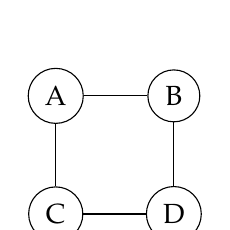
\begin{tikzpicture}[node distance=1.5cm, auto]
    \node[draw, circle] (A) {A};
    \node[draw, circle, right of=A] (B) {B};
    \node[draw, circle, below of=A] (C) {C};
    \node[draw, circle, right of=C] (D) {D};
    \draw (A) -- (B);
    \draw (A) -- (C);
    \draw (B) -- (D);
    \draw (C) -- (D);
\end{tikzpicture}
\end{center}

\textbf{DFS Pseudocode:}
\begin{lstlisting}
DFS(Graph, v):
    mark v as visited
    for all neighbors w of v:
        if w is not visited:
            DFS(Graph, w)
\end{lstlisting}

\subsubsection{DFS C++ Implementation}
\begin{lstlisting}[caption={DFS in C++ using an Adjacency List}]
#include <iostream>
#include <vector>
using namespace std;

void DFSUtil(const vector<vector<int>>& adjList, int v, vector<bool>& visited) {
    visited[v] = true;
    cout << v << " ";

    for (int neighbor : adjList[v]) {
        if (!visited[neighbor]) {
            DFSUtil(adjList, neighbor, visited);
        }
    }
}

void DFS(const vector<vector<int>>& adjList, int start) {
    int V = adjList.size();
    vector<bool> visited(V, false);
    DFSUtil(adjList, start, visited);
}

int main() {
    vector<vector<int>> adjList = {
        {1, 2},
        {0, 2, 3},
        {0, 1, 3},
        {1, 2}
    };
    cout << "DFS Traversal starting from vertex 0:\n";
    DFS(adjList, 0);
    return 0;
}
\end{lstlisting}

\section{Spanning Trees}

\subsection{Definition}
A \textbf{spanning tree} of a connected, undirected graph is a subgraph that is a tree and connects all the vertices together. A graph can have multiple spanning trees.

\subsection{Properties of Spanning Trees}
\begin{itemize}
    \item A spanning tree of a graph with $n$ vertices has exactly $n - 1$ edges.
    \item It is a minimal connected subgraph of the graph.
    \item There is no cycle in a spanning tree.
    \item Removing any edge from a spanning tree disconnects the graph.
    \item A connected graph with $n$ vertices and $n - 1$ edges is a tree.
\end{itemize}

\subsection{Minimum Spanning Tree (MST)}
A \textbf{minimum spanning tree} is a spanning tree whose sum of edge weights is the smallest among all possible spanning trees of the graph.

\textbf{Applications:}
\begin{itemize}
    \item Network design (e.g., electrical grid, computer networks)
    \item Approximation algorithms
    \item Clustering in machine learning
\end{itemize}

\textbf{Common Algorithms:}
\begin{itemize}
    \item \textbf{Kruskal's Algorithm}: Adds edges in increasing order of weight, skipping cycles.
    \item \textbf{Prim's Algorithm}: Grows the MST one vertex at a time from a starting node.
\end{itemize}

\subsection{Maximum Spanning Tree}
A \textbf{maximum spanning tree} is similar to an MST but maximizes the total edge weight. It is useful in certain optimization problems where higher weights are preferred (e.g., maximizing reliability or capacity).

\subsection{Comparison}
\begin{center}
\begin{tabular}{|l|l|l|}
\hline
\textbf{Aspect} & \textbf{MST} & \textbf{MaxST} \\
\hline
Objective & Minimize total weight & Maximize total weight \\
\hline
Used In & Cost-saving applications & Capacity or reliability maximization \\
\hline
Algorithm Change & Sort edges by increasing weight & Sort edges by decreasing weight \\
\hline
\end{tabular}
\end{center}
A \textbf{spanning tree} of a graph is a subgraph that includes all the vertices of the original graph, is connected, and has no cycles. In an undirected graph, any spanning tree will have exactly \( V - 1 \) edges.

\subsubsection{Example and Diagram of a Spanning Tree}
Given an undirected graph:
\begin{center}
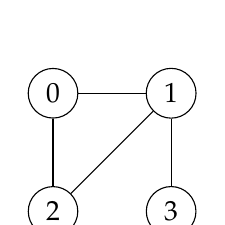
\begin{tikzpicture}[node distance=1.5cm, auto]
    \node[draw, circle] (0) {0};
    \node[draw, circle, right of=0] (1) {1};
    \node[draw, circle, below of=0] (2) {2};
    \node[draw, circle, right of=2] (3) {3};
    \draw (0) -- (1);
    \draw (0) -- (2);
    \draw (1) -- (2);
    \draw (1) -- (3);
\end{tikzpicture}
\end{center}

A possible spanning tree for the graph is:
\begin{center}
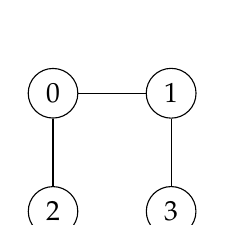
\begin{tikzpicture}[node distance=1.5cm, auto]
    \node[draw, circle] (0) {0};
    \node[draw, circle, right of=0] (1) {1};
    \node[draw, circle, below of=0] (2) {2};
    \node[draw, circle, right of=2] (3) {3};
    \draw (0) -- (1);
    \draw (0) -- (2);
    \draw (1) -- (3);
\end{tikzpicture}
\end{center}

\subsubsection{Spanning Tree via BFS (C++ Implementation)}
Below is an example of using BFS to generate a spanning tree from a connected undirected graph.
\begin{lstlisting}[caption={Spanning Tree using BFS in C++}]
#include <iostream>
#include <vector>
#include <queue>
using namespace std;

void spanningTreeBFS(const vector<vector<int>>& adjList, int start) {
    int V = adjList.size();
    vector<bool> visited(V, false);
    vector<int> parent(V, -1);
    queue<int> q;

    visited[start] = true;
    q.push(start);

    while (!q.empty()) {
        int u = q.front();
        q.pop();

        for (int v : adjList[u]) {
            if (!visited[v]) {
                visited[v] = true;
                parent[v] = u;
                q.push(v);
            }
        }
    }

    cout << "Spanning Tree (parent representation):\n";
    for (int i = 0; i < V; i++) {
        if (parent[i] != -1)
            cout << parent[i] << " - " << i << "\n";
    }
}

int main() {
    vector<vector<int>> adjList = {
        {1, 2},
        {0, 2, 3},
        {0, 1, 3},
        {1, 2}
    };
    spanningTreeBFS(adjList, 0);
    return 0;
}
\end{lstlisting}

\section{Diagrams for Graph Representations}

In this section, we provide visual diagrams for the two primary representations of graphs: the adjacency matrix and the adjacency list. We will consider a sample graph with vertices \(0,1,2,3\) and edges \(\{0,1\}\), \(\{0,2\}\), \(\{1,2\}\), and \(\{1,3\}\).

\subsection{Adjacency Matrix Diagram}
The adjacency matrix for the sample graph is a \(4 \times 4\) matrix where the rows and columns correspond to the vertices. A value of \(1\) indicates the presence of an edge between the corresponding vertices, and a value of \(0\) indicates no edge.

\begin{center}
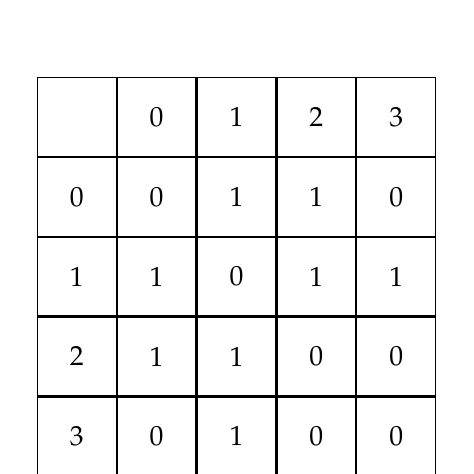
\begin{tikzpicture}
  \matrix[matrix of nodes,
          nodes in empty cells,
          nodes={draw, minimum size=1cm, anchor=center},
          column sep=0pt,
          row sep=0pt
         ] {
         \ & 0 & 1 & 2 & 3 \\
         0 & 0 & 1 & 1 & 0 \\
         1 & 1 & 0 & 1 & 1 \\
         2 & 1 & 1 & 0 & 0 \\
         3 & 0 & 1 & 0 & 0 \\
  };
\end{tikzpicture}
\end{center}

\subsection{Adjacency List Diagram}
The adjacency list represents the graph by listing each vertex followed by the vertices adjacent to it. For our sample graph, the adjacency list is as follows:
\[
\begin{array}{l}
0: \quad 1 \rightarrow 2 \\
1: \quad 0 \rightarrow 2 \rightarrow 3 \\
2: \quad 0 \rightarrow 1 \\
3: \quad 1 \\
\end{array}
\]

The diagram below visually represents this structure:

\begin{center}
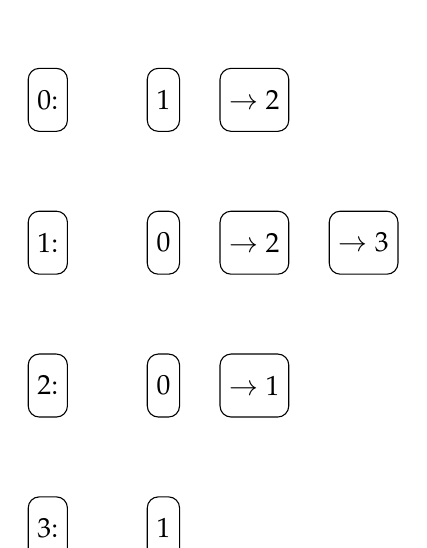
\begin{tikzpicture}[node distance=1cm, every node/.style={draw, rectangle, rounded corners, minimum height=0.8cm}]
    % List nodes for vertex labels
    \node (v0) {0:};
    \node[right=1cm of v0] (v0list) {1};
    \node[right=0.5cm of v0list] (v0list2) {$\rightarrow$ 2};

    \node (v1) [below=of v0] {1:};
    \node[right=1cm of v1] (v1list) {0};
    \node[right=0.5cm of v1list] (v1list2) {$\rightarrow$ 2};
    \node[right=0.5cm of v1list2] (v1list3) {$\rightarrow$ 3};

    \node (v2) [below=of v1] {2:};
    \node[right=1cm of v2] (v2list) {0};
    \node[right=0.5cm of v2list] (v2list2) {$\rightarrow$ 1};

    \node (v3) [below=of v2] {3:};
    \node[right=1cm of v3] (v3list) {1};
\end{tikzpicture}
\end{center}

These diagrams help in visualizing the structural differences between the two common graph representations. The matrix provides a compact, fixed-size representation (especially useful for dense graphs), while the list provides a more flexible and space-efficient representation (especially useful for sparse graphs).

\section{Conclusion}
This chapter has provided an in-depth exploration of graph data structures and algorithms. We began with the theoretical foundations, key terminology, and useful formulas.
\part{Searching and Sorting}
\chapter{Searching Algorithms}

This chapter explains fundamental searching algorithms with step-by-step examples, complete C++ implementations using the \texttt{listings} package, and diagrams illustrating the search process.

\section{Linear Search}
Linear Search scans each element of the array sequentially until the target value is found or the end of the array is reached.

\subsection{Explanation}
Given an array \( arr \) of size \( n \) and a target value, the algorithm starts at the first element and compares each element with the target. If a match is found, the index is returned; otherwise, it continues until all elements are checked.

\subsection{C++ Code Example}
\begin{lstlisting}[language=C++, caption={Linear Search Implementation}]
#include <bits/stdc++.h>
using namespace std;

int linearSearch(const vector<int>& arr, int target) {
    for (int i = 0; i < arr.size(); i++) {
        if (arr[i] == target)
            return i; // Target found at index i
    }
    return -1; // Target not found
}
int main() {
    vector<int> arr = {3, 8, 2, 5, 9, 1};
    int target = 5;
    int index = linearSearch(arr, target);
    if (index != -1)
        cout << "Target " << target << " at index " << index << "\n";
    else
        cout << "Target " << target << " not found." << "\n";
        
    return 0;
}
\end{lstlisting}

\subsection{Diagram: Linear Search Process}
The following diagram shows how Linear Search traverses the array sequentially.

\begin{figure}[H]
\centering
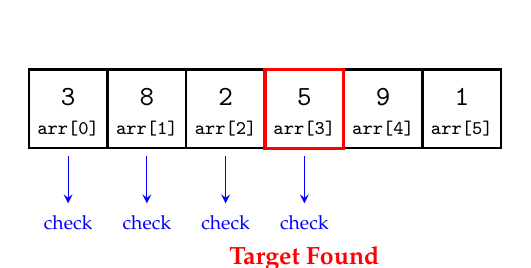
\begin{tikzpicture}[>=stealth, node distance=1.2cm]
  % Draw array boxes with values
  \foreach \i/\val in {0/3, 1/8, 2/2, 3/5, 4/9, 5/1} {
    \draw[thick] (\i,0) rectangle (\i+1,1);
    \node at (\i+0.5,0.65) {\texttt{\val}};
    \node at (\i+0.5,0.25) {\scriptsize\texttt{arr[\i]}};
  }

  % Highlight target element (assume target is at index 3)
  \draw[very thick, red] (3,0) rectangle (4,1);

  % Draw arrows and labels below each element checked
  \foreach \i in {0,...,3} {
    \draw[->, blue] (\i+0.5, -0.1) -- (\i+0.5, -0.7);
    \node[blue] at (\i+0.5, -0.95) {\scriptsize check};
  }

  % Target found text
  \node[red, font=\small\bfseries] at (3.5, -1.4) {Target Found};
\end{tikzpicture}
\caption{Linear Search: Sequentially checking each element}
\end{figure}


\section{Binary Search}
Binary Search is a highly efficient algorithm for searching in a sorted array. It repeatedly divides the search interval in half.

\subsection{Explanation}
Given a sorted array \( arr \) of size \( n \) and a target value, Binary Search works as follows:
\begin{enumerate}
  \item Set two pointers, \( \text{low} = 0 \) and \( \text{high} = n-1 \).
  \item Find the middle index: \( \text{mid} = \lfloor (\text{low} + \text{high})/2 \rfloor \).
  \item If \( arr[\text{mid}] \) equals the target, return \( \text{mid} \).
  \item If the target is less than \( arr[\text{mid}] \), repeat the search in the left subarray.
  \item Otherwise, repeat the search in the right subarray.
\end{enumerate}

\subsection{C++ Code Example}
\begin{lstlisting}[language=C++, caption={Binary Search Implementation}]
#include <bits/stdc++.h>
using namespace std;

int binarySearch(const vector<int>& arr, int target) {
    int low = 0, high = arr.size() - 1;
    while (low <= high) {
        int mid = low + (high - low) / 2;
        if (arr[mid] == target)
            return mid; // Target found
        else if (arr[mid] < target)
            low = mid + 1;
        else
            high = mid - 1;
    }
    return -1; // Target not found
}
int main() {
    vector<int> arr = {1, 3, 5, 7, 9, 11};
    int target = 7;
    int index = binarySearch(arr, target);
    if (index != -1)
        cout << "Target " << target << " at index " << index << "\n";
    else
        cout << "Target " << target << " not found." << "\n";
    return 0;
}
\end{lstlisting}

\subsection{Diagram: Binary Search Process}
The following diagram illustrates how Binary Search halves the search interval at each step.

\begin{figure}[H]
\centering
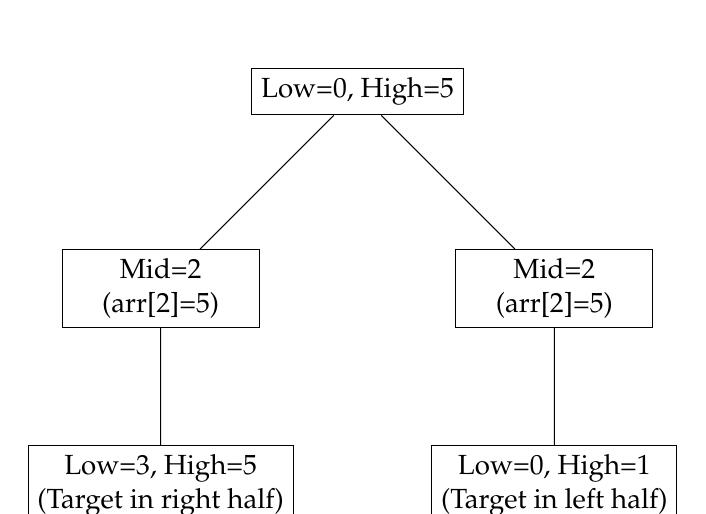
\begin{tikzpicture}[grow=down, level distance=2.5cm, sibling distance=5cm,
  every node/.style={draw, rectangle, align=center, minimum width=2.5cm}]
  \node {Low=0, High=5}
    child { node {Mid=2\\(arr[2]=5)} 
      child { node {Low=3, High=5\\(Target in right half)} } }
    child { node {Mid=2\\(arr[2]=5)} 
      child { node {Low=0, High=1\\(Target in left half)} } };
\end{tikzpicture}
\caption{Binary Search: Halving the search interval}
\end{figure}

\subsection{Step-by-Step Example of Binary Search}
Consider a sorted array: \([1, 3, 5, 7, 9, 11]\) and a target value of 7.
\begin{enumerate}
  \item Initialize: \(\text{low} = 0\), \(\text{high} = 5\). Compute \(\text{mid} = 2\). \(arr[2] = 5\). Since \(5 < 7\), move to the right half.
  \item Update: \(\text{low} = 3\), \(\text{high} = 5\). Compute \(\text{mid} = 4\). \(arr[4] = 9\). Since \(9 > 7\), move to the left half.
  \item Update: \(\text{low} = 3\), \(\text{high} = 3\). Compute \(\text{mid} = 3\). \(arr[3] = 7\). Target found at index 3.
\end{enumerate}

\section{Exponential Search}
Exponential Search is useful for unbounded or large sorted arrays. It first finds a range where the target may reside by repeatedly doubling the index, then performs a Binary Search in that range.

\subsection{Explanation}
Given a sorted array \( arr \) of size \( n \) and a target value:
\begin{enumerate}
  \item If \( arr[0] \) is the target, return index 0.
  \item Otherwise, initialize index \( i = 1 \) and double \( i \) until \( arr[i] > \) target or \( i \geq n \).
  \item Perform Binary Search on the subarray from \( i/2 \) to \( \min(i, n-1) \).
\end{enumerate}

\subsection{C++ Code Example}
\begin{lstlisting}[language=C++, caption={Exponential Search Implementation}]
#include <bits/stdc++.h>
using namespace std;

int binarySearch(const vector<int>& arr, int low, int high, int target) {
    while (low <= high) {
        int mid = low + (high - low) / 2;
        if (arr[mid] == target)
            return mid;
        else if (arr[mid] < target)
            low = mid + 1;
        else
            high = mid - 1;
    }
    return -1;
}

int exponentialSearch(const vector<int>& arr, int target) {
    int n = arr.size();
    if (n == 0) return -1;
    if (arr[0] == target) return 0;
    int i = 1;
    while (i < n && arr[i] <= target)
        i *= 2;
    return binarySearch(arr, i / 2, min(i, n - 1), target);
}
int main() {
    vector<int> arr = {1, 3, 5, 7, 9, 11, 13, 15, 17, 19};
    int target = 15;
    int index = exponentialSearch(arr, target);
    if (index != -1)
        cout << "Target " << target << " at index " << index << "\n";
    else
        cout << "Target " << target << " not found." << "\n"; 
    return 0;
}
\end{lstlisting}

\subsection{Diagram: Exponential Search Process}
The diagram below shows how the algorithm doubles the index until the range is found, then performs Binary Search.

\begin{figure}[H]
\centering
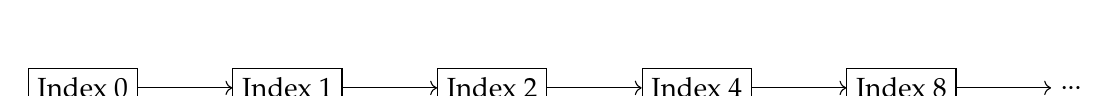
\begin{tikzpicture}[node distance=1.2cm]
    \node[draw, rectangle] (i0) {Index 0};
    \node[draw, rectangle, right=of i0] (i1) {Index 1};
    \node[draw, rectangle, right=of i1] (i2) {Index 2};
    \node[draw, rectangle, right=of i2] (i4) {Index 4};
    \node[draw, rectangle, right=of i4] (i8) {Index 8};
    \node[right=of i8] (dots) {...};
    \draw[->] (i0) -- (i1);
    \draw[->] (i1) -- (i2);
    \draw[->] (i2) -- (i4);
    \draw[->] (i4) -- (i8);
    \draw[->] (i8) -- (dots);
\end{tikzpicture}
\caption{Exponential Search: Doubling indices to find the search range}
\end{figure}

\section{Interpolation Search}
Interpolation Search improves upon Binary Search for uniformly distributed arrays by estimating the position of the target using the values at the endpoints.

\subsection{Explanation}
For a sorted array \( arr \) of size \( n \) and target value:
\[
\text{pos} = \text{low} + \frac{(target - arr[low]) \times (high - low)}{arr[high] - arr[low]}
\]
This position is used to probe the array. If the target is found at \(\text{pos}\), the index is returned; otherwise, the search continues in the appropriate subarray.

\subsection{C++ Code Example}
\begin{lstlisting}[language=C++, caption={Interpolation Search Implementation}]
#include <bits/stdc++.h>
using namespace std;

int interpolationSearch(const vector<int>& arr, int target) {
    int low = 0, high = arr.size() - 1;
    while (low <= high && target >= arr[low] && target <= arr[high]) {
        if (low == high) {
            if (arr[low] == target) return low;
            return -1;
        }
        int pos = low + ((double)(high - low) / (arr[high] - arr[low])) * (target - arr[low]);
        
        if (arr[pos] == target)
            return pos;
        if (arr[pos] < target)
            low = pos + 1;
        else
            high = pos - 1;
    }
    return -1;
}

int main() {
    vector<int> arr = {10, 20, 30, 40, 50, 60, 70, 80, 90};
    int target = 70;
    int index = interpolationSearch(arr, target);
    
    if (index != -1)
        cout << "Target " << target << " at index " << index << "\n";
    else
        cout << "Target " << target << " not found." << "\n";
        
    return 0;
}
\end{lstlisting}

\paragraph{Time Complexity Analysis:}
\begin{itemize}
  \item \textbf{Average Case:} \(O(\log \log n)\) for uniformly distributed data.
  \item \textbf{Worst Case:} \(O(n)\) when the data is not uniformly distributed.
\end{itemize}

\section{Conclusion}
In this chapter, we explored several searching algorithms:
\begin{itemize}
  \item \textbf{Linear Search}: Simple and works on unsorted data (\(O(n)\)).
  \item \textbf{Binary Search}: Efficient on sorted arrays (\(O(\log n)\)).
  \item \textbf{Exponential Search}: Finds the range for Binary Search in unbounded arrays (\(O(\log n)\)).
  \item \textbf{Interpolation Search}: Optimized for uniformly distributed data (\(O(\log \log n)\) on average).
\end{itemize}

Each algorithm has its strengths and is applicable to different scenarios. Understanding these algorithms and their performance characteristics is crucial for selecting the most appropriate method for your needs.

\chapter{Sorting Algorithms}

This chapter provides detailed C++ implementations of several important sorting algorithms. Each algorithm is explained with code examples using the \texttt{listings} package.

\section{Bubble Sort}
Bubble Sort repeatedly compares adjacent elements and swaps them if they are in the wrong order. It is simple but inefficient for large datasets.

\begin{lstlisting}[language=C++, caption={Bubble Sort Implementation}]
void bubbleSort(vector<int>& arr) {
    int n = arr.size();
    for (int i = 0; i < n - 1; i++) {
        bool swapped = false;
        for (int j = 0; j < n - i - 1; j++) {
            if (arr[j] > arr[j+1]) {
                swap(arr[j], arr[j+1]);
                swapped = true;
            }
        }
        if (!swapped)
            break; // Array is sorted
    }
}
\end{lstlisting}

\section{Insertion Sort}
Insertion Sort builds the sorted array one element at a time by comparing each new element with the already sorted elements.

\begin{lstlisting}[language=C++, caption={Insertion Sort Implementation}]
void insertionSort(vector<int>& arr) {
    int n = arr.size();
    for (int i = 1; i < n; i++) {
        int key = arr[i];
        int j = i - 1;
        while (j >= 0 && arr[j] > key) {
            arr[j+1] = arr[j];
            j--;
        }
        arr[j+1] = key;
    }
}
\end{lstlisting}

\section{Selection Sort}
Selection Sort repeatedly finds the minimum element from the unsorted portion and swaps it with the first unsorted element.

\begin{lstlisting}[language=C++, caption={Selection Sort Implementation}]
void selectionSort(vector<int>& arr) {
    int n = arr.size();
    for (int i = 0; i < n - 1; i++) {
        int minIdx = i;
        for (int j = i + 1; j < n; j++) {
            if (arr[j] < arr[minIdx])
                minIdx = j;
        }
        swap(arr[i], arr[minIdx]);
    }
}
\end{lstlisting}

\section{Counting Sort}
Counting Sort works efficiently when the range of input data (\(k\)) is not significantly greater than the number of elements (\(n\)). It counts the occurrences of each value and then reconstructs the sorted array.

\begin{lstlisting}[language=C++, caption={Counting Sort Implementation}]
void countingSort(vector<int>& arr) {
    int n = arr.size();
    int maxVal = *max_element(arr.begin(), arr.end());
    vector<int> count(maxVal + 1, 0);
    for (int i = 0; i < n; i++) {
        count[arr[i]]++;
    }
    int index = 0;
    for (int i = 0; i <= maxVal; i++) {
        while (count[i]-- > 0) {
            arr[index++] = i;
        }
    }
}
\end{lstlisting}

\paragraph{Time Complexity Analysis:}
\begin{itemize}
  \item Counting frequency: \(O(n)\)
  \item Populating the sorted array: \(O(k)\)
\end{itemize}
Overall, the expected time complexity is \(O(n + k)\), with space complexity \(O(k)\).

\section{Radix Sort}
Radix Sort is a non-comparative sorting algorithm that sorts numbers digit by digit using Counting Sort as a subroutine.

\begin{lstlisting}[language=C++, caption={Radix Sort Implementation}]
int getMax(const vector<int>& arr) {
    return *max_element(arr.begin(), arr.end());
}
void countingSortByDigit(vector<int>& arr, int exp) {
    int n = arr.size();
    vector<int> output(n);
    vector<int> count(10, 0);
    for (int i = 0; i < n; i++)
        count[(arr[i] / exp) % 10]++;
    for (int i = 1; i < 10; i++)
        count[i] += count[i - 1];
    for (int i = n - 1; i >= 0; i--) {
        output[count[(arr[i] / exp) % 10] - 1] = arr[i];
        count[(arr[i] / exp) % 10]--;
    }
    for (int i = 0; i < n; i++)
        arr[i] = output[i];
}
void radixSort(vector<int>& arr) {
    int maxVal = getMax(arr);
    for (int exp = 1; maxVal / exp > 0; exp *= 10)
        countingSortByDigit(arr, exp);
}
\end{lstlisting}

\paragraph{Time Complexity Analysis:}
\[
O(d(n + b)) \quad \text{where } d \text{ is the number of digits and } b \text{ is the base (typically 10).}
\]
For decimal numbers, this is often written as \(O(n \log_{10} k)\).

\section{Timsort}
Timsort is a hybrid sorting algorithm derived from merge sort and insertion sort. It is used in Python’s sort and Java’s Arrays.sort() for objects. Below is a simplified version in C++.

\begin{lstlisting}[language=C++, caption={Timsort Implementation (Simplified)}]
const int RUN = 32;
void insertionSort(vector<int>& arr, int left, int right) {
    for (int i = left + 1; i <= right; i++) {
        int temp = arr[i];
        int j = i - 1;
        while (j >= left && arr[j] > temp) {
            arr[j+1] = arr[j];
            j--;
        }
        arr[j+1] = temp;
    }
}
void merge(vector<int>& arr, int l, int m, int r) {
    int len1 = m - l + 1, len2 = r - m;
    vector<int> leftArr(len1), rightArr(len2);
    for (int i = 0; i < len1; i++) leftArr[i] = arr[l + i];
    for (int i = 0; i < len2; i++) rightArr[i] = arr[m + 1 + i];
    int i = 0, j = 0, k = l;
    while (i < len1 && j < len2) {
        if (leftArr[i] <= rightArr[j]) arr[k++] = leftArr[i++];
        else arr[k++] = rightArr[j++];
    }
    while (i < len1) arr[k++] = leftArr[i++];
    while (j < len2) arr[k++] = rightArr[j++];
}
void timSort(vector<int>& arr, int n) {
    for (int i = 0; i < n; i += RUN) {
        insertionSort(arr, i, min(i + RUN - 1, n - 1));
    }
    for (int size = RUN; size < n; size *= 2) {
        for (int left = 0; left < n; left += 2 * size) {
            int mid = left + size - 1;
            int right = min(left + 2 * size - 1, n - 1);
            if (mid < right) merge(arr, left, mid, right);
        }
    }
}
\end{lstlisting}

\paragraph{Time Complexity Analysis:}
\begin{itemize}
  \item Best Case (nearly sorted): \(O(n)\)
  \item Worst Case: \(O(n \log n)\)
  \item Timsort adapts to the natural order in the data.
\end{itemize}

\section{Merge Sort}
Merge Sort is a classic divide-and-conquer algorithm. It divides an array into two halves, recursively sorts each half, and then merges the two sorted halves.

\subsection{Merge Sort Implementation in C++}
\begin{lstlisting}[language=C++, caption={Merge Sort Implementation}]
#include <bits/stdc++.h>
using namespace std;

void merge(vector<int>& arr, int left, int mid, int right) {
    int n1 = mid - left + 1; 
    int n2 = right - mid;
    vector<int> L(n1), R(n2);
    for (int i = 0; i < n1; i++)
        L[i] = arr[left + i];
    for (int j = 0; j < n2; j++)
        R[j] = arr[mid + 1 + j];
    int i = 0, j = 0, k = left;
    while (i < n1 && j < n2) {
        if (L[i] <= R[j])
            arr[k++] = L[i++];
        else
            arr[k++] = R[j++];
    }
    while (i < n1)
        arr[k++] = L[i++];
    while (j < n2)
        arr[k++] = R[j++];
}
void mergeSort(vector<int>& arr, int left, int right) {
    if (left < right) {
        int mid = left + (right - left) / 2;
        mergeSort(arr, left, mid);
        mergeSort(arr, mid + 1, right);
        merge(arr, left, mid, right);
    }
}
\end{lstlisting}

\subsection{Example Usage}
\begin{lstlisting}[language=C++, caption={Using Merge Sort}]
int main() {
    vector<int> arr = {38, 27, 43, 3, 9, 82, 10};
    int n = arr.size();
    
    mergeSort(arr, 0, n - 1);
    
    cout << "Sorted array: ";
    for (int x : arr)
        cout << x << " ";
    cout << endl;
    
    return 0;
}
\end{lstlisting}

\subsection{Time Complexity Analysis}
Merge Sort divides the array into halves and then merges them. Its recurrence relation is:
\[
T(n) = 2T\left(\frac{n}{2}\right) + O(n)
\]
which solves to:
\[
T(n) = O(n \log n)
\]
Thus, Merge Sort has a time complexity of \(O(n \log n)\) in all cases.

\paragraph{Space Complexity:}  
Merge Sort requires additional space for temporary arrays during merging:
\[
O(n)
\]

\section*{Summary}
Each sorting algorithm has its trade-offs in terms of time and space complexity:
\begin{itemize}
  \item \textbf{Bubble Sort}: \(O(n^2)\) worst-case, very simple but inefficient.
  \item \textbf{Insertion Sort}: \(O(n^2)\) worst-case, \(O(n)\) best-case, efficient for nearly sorted data.
  \item \textbf{Selection Sort}: \(O(n^2)\) consistently, few swaps.
  \item \textbf{Counting Sort}: \(O(n + k)\) time, where \(k\) is the range of the input.
  \item \textbf{Radix Sort}: \(O(n \log_{10} k)\) for decimal numbers.
  \item \textbf{Timsort}: Hybrid algorithm with \(O(n)\) best-case and \(O(n \log n)\) worst-case.
\end{itemize}

% Chapter 21: DSA Coding Questions (Reorganized)
\chapter{DSA Coding Questions}

% ----------------------------
% Company-wise and Pattern Highlights
% ----------------------------
\section*{Top Interview Topics by Company}
\begin{itemize}
  \item \textbf{Google}: Trees, Graphs, DP, Backtracking, Tries, System Design
  \item \textbf{Amazon}: Arrays, Strings, Hashing, Sliding Window, Greedy
  \item \textbf{Microsoft}: DP, Graphs, Trees, Bit Manipulation
  \item \textbf{Adobe}: Heap, Stack, Recursion, Trees
  \item \textbf{Flipkart}: Greedy, Hashing, Priority Queue, Segment Tree
  \item \textbf{Meta (Facebook)}: BFS/DFS, Backtracking, Sliding Window, Graphs
  \item \textbf{Netflix}: Dynamic Programming, Interval Problems, System Design
  \item \textbf{Uber}: Priority Queue, Shortest Path, Greedy
  \item \textbf{Bloomberg}: Hash Maps, Stack, Graphs
  \item \textbf{TCS/Wipro/Infosys}: Basics of Arrays, Searching, Sorting, OOP, Recursion
\end{itemize}

\section*{Core DSA Patterns}
\begin{itemize}
  \item Sliding Window, Two Pointers
  \item Fast and Slow Pointers, Binary Search on Answer
  \item BFS / DFS / Backtracking
  \item Recursion + Memoization
  \item Prefix Sum, Hashing, Greedy
  \item Stack (Span/NGE/Histograms)
\end{itemize}

% ----------------------------
% Reorganized by Patterns and Topics
% ----------------------------

\section*{\ Arrays and Strings}
\begin{itemize}
  \item \textbf{[Easy]} Reverse an array
  \item \textbf{[Easy]} Find max and min in array
  \item \textbf{[Easy]} Move all zeros to the end
  \item \textbf{[Medium]} Union and Intersection of two arrays \textit{(Amazon)}
  \item \textbf{[Medium]} Kadane’s Algorithm – Max Subarray Sum \textit{(Google)}
  \item \textbf{[Medium]} Longest substring without repeating characters \textit{(Meta)}
  \item \textbf{[Medium]} Anagram check using hashing \textit{(Bloomberg)}
  \item \textbf{[Hard]} Z-algorithm for pattern matching \textit{(Adobe)}
\end{itemize}

\section*{\ Searching and Sorting}
\begin{itemize}
  \item Linear Search / Binary Search
  \item Search in Rotated Sorted Array \textit{(Microsoft)}
  \item Floor and Ceil of a number \textit{(Flipkart)}
  \item Merge Sort, Quick Sort
  \item Count Inversions in array \textit{(Amazon)}
\end{itemize}

\section*{\ Two Pointers / Sliding Window}
\begin{itemize}
  \item Maximum sum subarray of size K
  \item Longest substring with at most K distinct characters
  \item Minimum window substring \textit{(Amazon)}
  \item Trapping Rain Water \textit{(Google)}
\end{itemize}

\section*{\ Linked Lists}
\begin{itemize}
  \item Reverse a linked list
  \item Detect loop using Floyd’s cycle
  \item Merge 2 sorted linked lists
  \item Check if LL is palindrome \textit{(Microsoft)}
  \item Clone LL with random pointer \textit{(Amazon)}
\end{itemize}

\section*{\ Stack and Queue}
\begin{itemize}
  \item Valid Parentheses Checker
  \item Next Greater Element \textit{(Adobe)}
  \item Min Stack Design \textit{(Google)}
  \item Largest Rectangle in Histogram \textit{(Facebook)}
  \item LRU Cache Implementation
\end{itemize}

\section*{\ Trees and BST}
\begin{itemize}
  \item Traversals: Inorder, Preorder, Postorder
  \item Diameter of Binary Tree \textit{(Google)}
  \item Construct Tree from Inorder and Preorder
  \item Lowest Common Ancestor (LCA)
  \item BST Insertion, Deletion, Search
  \item Kth Smallest/Largest in BST
\end{itemize}

\section*{\ Graphs}
\begin{itemize}
  \item BFS and DFS Traversal
  \item Cycle Detection in Directed / Undirected Graph
  \item Topological Sort
  \item Dijkstra’s Algorithm, Bellman-Ford
  \item Number of Islands \textit{(Amazon)}
  \item Clone a Graph
\end{itemize}

\section*{\ Recursion and Backtracking}
\begin{itemize}
  \item Subsets / Permutations / Combinations
  \item N-Queens Problem \textit{(Facebook)}
  \item Sudoku Solver
  \item Word Search
  \item Generate Balanced Parentheses
\end{itemize}

\section*{\ Greedy Algorithms}
\begin{itemize}
  \item Activity Selection
  \item Fractional Knapsack
  \item Job Scheduling with Deadlines \textit{(Flipkart)}
  \item Minimum Coins for Change
  \item Gas Station Circle
\end{itemize}

\section*{\ Heap / Priority Queue}
\begin{itemize}
  \item Heapify, Min/Max Heap
  \item Kth Largest Element \textit{(Amazon)}
  \item Merge K Sorted Lists
  \item Median of a Stream
  \item Reorganize String using Heap
\end{itemize}

\section*{\ Dynamic Programming (DP)}
\begin{itemize}
  \item Fibonacci (Memoization)
  \item 0/1 Knapsack
  \item Longest Common Subsequence (LCS)
  \item Longest Increasing Subsequence (LIS)
  \item Coin Change
  \item Edit Distance
  \item Palindromic Substrings Count \textit{(Amazon)}
\end{itemize}

% End of Chapter

\chapter{C++ Template}
\label{chap:cpp-template}

\section{Basic Template}

This is the basic template that anyone can use to write the code in c++.

\begin{lstlisting}[language=C++, caption={Main C++ Template}]
#include <bits/stdc++.h>

using namespace std;

void solve(){
    //Code Here....
}
void init_code(){
    ios_base :: sync_with_stdio(false);
    cin.tie(nullptr);
    cout.tie(nullptr);
}
int main(){
    init_code();
    solve();
    return 0;
}

\end{lstlisting}
\newpage
\section{Debugging Template}
\begin{lstlisting}[language=C++, caption={Debugging Template}]
template < class c > struct rge {
    c b, e;
};
template < class c > rge<c> range(c i, c j){
    return rge<c>{i, j};
}
template < class c > auto dud(c* x) -> decltype(cerr << *x, 0);
template < class c > char dud(...);

struct debug {
    ~debug() { cerr << endl; }
    template < class c > typename enable_if<sizeof dud<c>(0) != 1, debug&>::type operator<<(c i) {
        cerr << boolalpha << i;
        return * this;
    }
    template < class c > typename enable_if<sizeof dud<c>(0) == 1, debug&>::type operator<<(c i) {
        return * this << range(begin(i), end(i)); 
    }
    template < class c, class b > debug & operator << (pair < b, c > d) {
        return * this << "(" << d.first << ", " << d.second << ")";
    }
    template < class c > debug & operator <<(rge<c> d) {
        *this << "[";
        for (auto it = d.b; it != d.e; ++it)
            *this << ", " + 2 * (it == d.b) << *it;
        return * this << "]";
    }
};  
#define imie(...) " [" << #__VA_ARGS__ " : " << (__VA_ARGS__) << "]"
\end{lstlisting}
\newpage
\section{Combined Template}

Here is a combined template for development that includes both the main structure and debugging utilities.

\begin{lstlisting}[language=C++, caption={Combined Template}]
/*
*
*    Author : Girish Kumar Goyal.
*
*/

#include <bits/stdc++.h>

using namespace std;

template < class c > struct rge {
    c b, e;
};
template < class c > rge<c> range(c i, c j){
    return rge<c>{i, j};
}
template < class c > auto dud(c* x) -> decltype(cerr << *x, 0);
template < class c > char dud(...);
struct debug {
    ~debug() { cerr << endl; }
    template < class c > typename enable_if<sizeof dud<c>(0) != 1, debug&>::type operator<<(c i) {
        cerr << boolalpha << i;
        return * this;
    }
    template < class c > typename enable_if<sizeof dud<c>(0) == 1, debug&>::type operator<<(c i) {
        return * this << range(begin(i), end(i)); 
    }
    template < class c, class b > debug & operator << (pair < b, c > d) {
        return * this << "(" << d.first << ", " << d.second << ")";
    }
    template < class c > debug & operator <<(rge<c> d) {
        *this << "[";
        for (auto it = d.b; it != d.e; ++it)
            *this << ", " + 2 * (it == d.b) << *it;
        return * this << "]";
    }
};  
#define imie(...) " [" << #__VA_ARGS__ " : " << (__VA_ARGS__) << "]"

void solve(){
    //Code Here....
}
void init_code(){
    ios_base :: sync_with_stdio(false);
    cin.tie(nullptr);
    cout.tie(nullptr);
}
int main(){
    init_code();
    solve();
    return 0;
}
\end{lstlisting}
\section{Using the Debugging Template}

To use the debugging template, you can print variables or expressions during development by using the `debug()` object in combination with the `imie(...)` macro. This will output both the name of the variable and its value, which is extremely useful for tracing bugs.

\textbf{Syntax:}
\begin{lstlisting}[language=C++]
debug() << imie(variable1) << imie(variable2) << imie(expression);
\end{lstlisting}

\textbf{Example:}

Here's a complete example demonstrating the use of `debug()` and `imie(...)`:

\begin{lstlisting}[language=C++, caption={Debugging Example}]
void solve() {
    int a = 42;
    string s = "hello";
    vector<int> v = {1, 2, 3};
    
    debug() << imie(a) << imie(s) << imie(v);
}

void init_code(){
    ios_base :: sync_with_stdio(false);
    cin.tie(nullptr);
    cout.tie(nullptr);
}

int main(){
    init_code();
    solve();
    return 0;
}
\end{lstlisting}


\section{C++ program time calculation}

\textbf{Example:}

\begin{lstlisting}[language=C++, caption={CPP Code time Example}]
#include <bits/stdc++.h>

using namespace std;

void solve() {
    // Code here....
}

void init_code(){
    ios_base :: sync_with_stdio(false);
    cin.tie(nullptr);
    cout.tie(nullptr);
}

int main(){
    init_code();
    clock_t start, end;
    double cpu_time;
    start = clock();
    solve();
    cpu_time = ((double)(end - start)) / CLOCKS_PER_SEC;
    cout << cpu_time << "\n";
    return 0;
}
\end{lstlisting}

\newpage

\section{Test case generator program in C++}

\textbf{Example:}

Test case generator in c++ basically the code to generate random testcases like this.
\begin{verbatim}
2
5
1 2 3 4 5
4
2 3 1 43
\end{verbatim}

\begin{lstlisting}[language=C++, caption={Test case generator}]
#include<bits/stdc++.h>

using namespace std;

int naxTest = 20;
int naxArraySize = 50;
int naxValue = 5000;

vector<int> generateTestCase(int size, int maxValue) {
    vector<int> testCase(size);
    for (int i = 0; i < size; i++) {
        testCase[i] = rand() % maxValue + 1;
    }
    return testCase;
}

int main() {
    srand(time(0));
    int numTestCases = rand() % naxTest + 1;
    int maxArraySize = rand() % naxArraySize + 1;
    int maxValue = rand() % naxValue + 1;
    cout << numTestCases << "\n";
    for (int i = 0; i < numTestCases; i++) {
        int arraySize = rand() % maxArraySize + 1;
        cout << arraySize << "\n";
        vector<int> testCase = generateTestCase(arraySize, maxValue);
        // sort(testCase.begin(), testCase.end());
        for (int num : testCase) {
            cout << num << " ";
        }
        cout << "\n";
    }
    return 0;
}
\end{lstlisting}

\section{Script for stress testing of c++ code}

\textbf{Syntax:}
\begin{lstlisting}[language=C++]
./stress.sh
\end{lstlisting}

\textbf{Example:}

The following script automates compilation and stress testing of a C++ solution against generated test cases:

\begin{lstlisting}[style=bashstyle]
#!/bin/bash

black=$(tput setaf 0)
red=$(tput setaf 1)
green=$(tput setaf 2)
yellow=$(tput setaf 3)
blue=$(tput setaf 4)
magenta=$(tput setaf 5)
cyan=$(tput setaf 6)
white=$(tput setaf 7)
bold=$(tput bold)
reset=$(tput sgr0)
CPP_VERSION="c++17"
COMPILE_FLAGS="-Wall -Wextra -O2"
TEST_GEN_FILE="./stress_tester/test_gen.cpp"
MAIN_FILE="sol.cpp"
INPUT_FILE="in"
MAX_TESTS=5
TIME_LIMIT=2  # seconds per test case

usage() {
    echo -e "${bold}${cyan}Usage:${reset} $(basename "$0") [-t <num_tests>]"
    exit 1
}
while getopts "t:h" opt; do
    case $opt in
        t)
            MAX_TESTS="$OPTARG"
            ;;
        h)
            usage
            ;;
        *)
            usage
            ;;
    esac
done

log_info() {
    echo -e "${bold}${blue}[INFO]${reset} $1"
}
log_success() {
    echo -e "${bold}${green}[SUCCESS]${reset} $1"
}
log_error() {
    echo -e "${bold}${red}[ERROR]${reset} $1"
}
log_warning() {
    echo -e "${bold}${yellow}[WARNING]${reset} $1"
}
check_files() {
    echo ""
    echo "---------------------------------------------------------"
    local missing=0
    if [ ! -f "$MAIN_FILE" ]; then
        log_error "Main solution file ${yellow}$MAIN_FILE${reset} not found!"
        missing=1
    fi
    if [ ! -f "$TEST_GEN_FILE" ]; then
        log_error "Test case generator file ${yellow}$TEST_GEN_FILE${reset} not found!"
        missing=1
    fi
    if [ $missing -eq 1 ]; then
        exit 1
    fi
}
compile_file() {
    local src_file="$1"
    local exe_file="$2"
    local extra_flags="$3"
    log_info "Compiling ${yellow}$src_file${reset}..."
    local start_ns=$(date +%s%N)
    compile_output=$(g++ -std="$CPP_VERSION" $COMPILE_FLAGS $extra_flags "$src_file" -o "$exe_file" 2>&1)
    if [ $? -ne 0 ]; then
        log_error "Compilation failed for ${yellow}$src_file${reset}."
        echo -e "${red}Compiler output:${reset}"
        echo "$compile_output"
        exit 1
    fi
    local end_ns=$(date +%s%N)
    local compile_time_ns=$((end_ns - start_ns))
    local compile_time_ms=$(echo "scale=3; $compile_time_ns/1000000" | bc)
    log_success "Compiled ${yellow}$src_file${reset} to ${magenta}$exe_file${reset} in ${cyan}${compile_time_ms} ms${reset}."
}
stress_test() {
    local accepted=0
    local failed=0
    local total_test_time_ns=0
    echo -e "\n${bold}${red}Starting stress testing with ${yellow}$MAX_TESTS${red} test cases...${reset}"
    for (( i=1; i<=MAX_TESTS; i++ )); do
        echo -e "\n${bold}${blue}======= Test case #$i =======${reset}"
        ./generator > "$INPUT_FILE"
        echo -e "${bold}${magenta}[Input]:${reset}"
        cat "$INPUT_FILE"
        echo ""
        local start_ns=$(date +%s%N)
        output=$(timeout $TIME_LIMIT ./sol < "$INPUT_FILE" 2>&1)
        local ret_code=$?
        local end_ns=$(date +%s%N)
        local elapsed_ns=$((end_ns - start_ns))
        total_test_time_ns=$((total_test_time_ns + elapsed_ns))
        local elapsed_ms=$(echo "scale=3; $elapsed_ns/1000000" | bc)
        echo -e "${bold}${cyan}[Output]:${reset}"
        echo -e "$output"
        if [ $ret_code -eq 0 ]; then
            echo -e "${bold}${green}Test case #$i: Accepted in ${blue}${elapsed_ms} ms${reset}"
            ((accepted++))
        elif [ $ret_code -eq 124 ]; then
            echo -e "${bold}${red}Test case #$i: Time Limit Exceeded (TLE) after ${yellow}${elapsed_ms} ms${reset}"
            ((failed++))
        elif [ $ret_code -eq 137 ]; then
            echo -e "${bold}${red}Test case #$i: Memory Limit Exceeded (MLE) in ${yellow}${elapsed_ms} ms${reset}"
            ((failed++))
        elif [ $ret_code -eq 139 ]; then
            echo -e "${bold}${red}Test case #$i: Runtime Error (Segmentation Fault) in ${yellow}${elapsed_ms} ms${reset}"
            ((failed++))
        else
            echo -e "${bold}${red}Test case #$i: Runtime Error (exit code $ret_code) in ${yellow}${elapsed_ms} ms${reset}"
            ((failed++))
        fi
        echo -e "${bold}${white}=====================================${reset}"
    done
    total_test_time_ms=$(echo "scale=3; $total_test_time_ns/1000000" | bc)
    avg_time=$(echo "scale=3; $total_test_time_ms/$MAX_TESTS" | bc)
    echo -e "\n${bold}${red}Stress testing completed.${reset}"
    echo -e "${bold}${green}[Accepted]: $accepted${reset}    ${bold}${red}[Failed]: $failed${reset}"
    echo -e "${bold}${cyan}[Total testing time]: ${total_test_time_ms} ms${reset}"
    echo -e "${bold}${magenta}[Average time per test]: ${avg_time} ms${reset}"
    echo ""
}
check_files
compile_file "$TEST_GEN_FILE" "generator" ""
compile_file "$MAIN_FILE" "sol" ""
stress_test
\end{lstlisting}


\part{Commands}
\chapter{Linux Commands}
\label{ch:linux-commands}

%--------------------------------------------------
% Section 18.1: Basic Commands
%--------------------------------------------------
\section{Basic Linux Commands}

\begin{description}
  \item[\command{ls}] List directory contents.
  \item[\command{cd}] Change the current working directory.
  \item[\command{pwd}] Print the absolute path of the working directory.
  \item[\command{cp}] Copy files or directories.
  \item[\command{mv}] Move or rename files or directories.
  \item[\command{rm}] Remove files or directories.
  \item[\command{mkdir}] Create one or more directories.
  \item[\command{rmdir}] Remove empty directories.
  \item[\command{touch}] Create an empty file or update file timestamps.
  \item[\command{cat}] Concatenate and display file contents.
  \item[\command{less}] View file contents page by page.
  \item[\command{grep}] Search file(s) for lines matching a pattern.
  \item[\command{rm -rf}] Remove folder.
\end{description}

%--------------------------------------------------
% Section 18.2: Intermediate Commands
%--------------------------------------------------
\section{Intermediate Commands}

\begin{description}
  \item[\command{find}] Search for files in a directory hierarchy.
  \item[\command{chmod}] Change file or directory permissions.
  \item[\command{chown}] Change file or directory ownership.
  \item[\command{tar}] Create or extract archive files.
  \item[\command{zip}/\command{unzip}] Compress and decompress files in ZIP format.
  \item[\command{ssh}] Securely connect to a remote host.
  \item[\command{scp}] Securely copy files between hosts over SSH.
  \item[\command{rsync}] Efficiently synchronize files and directories.
  \item[\command{ps}] Display current active processes.
  \item[\command{kill}/\command{killall}] Terminate processes by PID or name.
  \item[\command{top}] Display dynamic real-time view of running processes.
  \item[\command{df}] Report filesystem disk space usage.
  \item[\command{du}] Estimate file and directory space usage.
  \item[\command{free}] Display memory usage statistics.
  \item[\command{head}/\command{tail}] Output the first or last part of files.
  \item[\command{awk}] Pattern scanning and processing language.
  \item[\command{sed}] Stream editor for filtering and transforming text.
\end{description}

%--------------------------------------------------
% Section 18.3: Advanced Commands
%--------------------------------------------------
\section{Advanced Commands}

\begin{description}
  \item[\command{htop}] Interactive process viewer with tree view and color coding.
  \item[\command{nmap}] Network exploration and security auditing tool.
  \item[\command{tcpdump}] Command-line packet analyzer.
  \item[\command{lsof}] List open files and the processes that opened them.
  \item[\command{strace}] Trace system calls and signals.
  \item[\command{iptables}/\command{nft}] Configure Linux kernel packet filtering rules.
  \item[\command{journalctl}] Query and display logs from the systemd journal.
  \item[\command{systemctl}] Control and inspect systemd services and units.
  \item[\command{curl}/\command{wget}] Transfer data to or from a server via various protocols.
  \item[\command{xargs}] Build and execute command lines from standard input.
  \item[\command{dd}] Convert and copy a file, often used for disk cloning.
  \item[\command{traceroute}] Print the route packets take to network host.
  \item[\command{dig}] DNS lookup utility.
  \item[\command{fuser}] Identify processes using files or sockets.
  \item[\command{screen}/\command{tmux}] Terminal multiplexers for session management.
  \item[\command{sudo apt-get autoremove --purge}] It helps clean up your system and free up disk space.
  \item[\command{sudo apt-get update}] It updates the local package index.
  \item[\command{sudo apt-get upgrade}] It upgrades all installed packages on your system to their latest versions.
\end{description}

\section{GIT Commands}

Git is a distributed version control system used to track changes in source code during software development. It allows multiple developers to work together efficiently and supports branching, merging, and collaboration through remote repositories (like GitHub or GitLab).

\subsection*{Basic Configuration}
Before using Git, configure your identity and preferred settings:

\begin{verbatim}
git config --global user.name "Your Name"
git config --global user.email "you@example.com"
git config --global init.defaultBranch main
git config --list   % View all configurations
\end{verbatim}

\subsection*{Common Git Commands}
\begin{description}
  \item[\command{git init}] Initializes a new Git repository in the current directory.
  \item[\command{git clone <url>}] Downloads a repository from a remote URL to your local machine.
  \item[\command{git add <file>}] Stages file(s) to be committed.
  \item[\command{git commit -m "message"}] Commits staged changes with a message.
  \item[\command{git status}] Displays the state of the working directory and staging area.
  \item[\command{git log}] Shows the commit history.
  \item[\command{git diff}] Shows the differences between files in the working directory and the index.
  \item[\command{git branch}] Lists all local branches.
  \item[\command{git branch -M main}] Renames the current branch to \command{main}.
  \item[\command{git checkout <branch>}] Switches to the specified branch.
  \item[\command{git checkout -b <branch>}] Creates a new branch and switches to it.
  \item[\command{git merge <branch>}] Merges changes from another branch into the current one.
  \item[\command{git remote add origin <url>}] Adds a remote repository (commonly GitHub).
  \item[\command{git remote set-url origin https://<token>@github.com/<user>/<repo>}] Changes the URL of the existing remote.
  \item[\command{git push}] Pushes local commits to the remote repository.
  \item[\command{git push origin main}] Pushes the \command{main} branch to the remote named \command{origin}.
  \item[\command{git push --set-upstream origin main}] Sets the upstream tracking for the current branch and pushes it.
  \item[\command{git pull}] Fetches from the remote repository and merges changes into the current branch.
  \item[\command{git pull origin main}] Pulls changes from the \command{main} branch of the remote \command{origin}.
  \item[\command{git reset --hard HEAD\textasciitilde1}] Resets the current branch to the previous commit, discarding all changes.
  \item[\command{git stash}] Temporarily saves uncommitted changes for later.
  \item[\command{git stash pop}] Restores the most recent stashed changes.
  \item[\command{git rm <file>}] Removes a file from the working directory and staging area.
  \item[\command{git tag <name>}] Tags a commit with a specified name.
  \item[\command{git fetch}] Retrieves changes from the remote without merging.
  \item[\command{git revert <commit>}] Reverts the changes of a specific commit.
  \item[\command{git show <commit>}] Displays information about a specific commit.
  \item[\command{git blame <file>}] Shows who changed what and when in a file.
\end{description}

\subsection*{Best Practices}
\begin{itemize}
  \item Commit often with clear messages.
  \item Use branches to manage different features or bug fixes.
  \item Use \command{git pull --rebase} to maintain a linear history when collaborating.
  \item Always check \command{git status} before committing or pushing.
\end{itemize}


\end{document}
